\documentclass[preprint,12pt]{elsarticle}

\usepackage{amsmath,amssymb,amsfonts,amsthm}
\usepackage{booktabs}
\usepackage{array}
\usepackage{algorithm}
\usepackage{algpseudocode}
\usepackage{enumitem}
\usepackage{geometry}
\usepackage{graphicx}
\usepackage{hyperref}
\hypersetup{hidelinks}
\usepackage{microtype}
\microtypesetup{expansion=false}
\setlength{\emergencystretch}{2em}
\usepackage{xcolor}
\usepackage{mathtools}
\usepackage{placeins}

\geometry{margin=1in}
\journal{Computer Methods in Applied Mechanics and Engineering}
\biboptions{numbers,sort&compress}

\newtheorem{definition}{Definition}
\newtheorem{proposition}{Proposition}
\newtheorem{theorem}{Theorem}
\newtheorem{remark}{Remark}
\newtheorem{assumption}{Assumption}

\newcommand{\R}{\mathbb{R}}
\newcommand{\Sph}{\mathbb{S}}
\newcommand{\Nc}{\mathcal{N}}
\newcommand{\Cc}{\mathcal{C}}
\newcommand{\Pc}{\mathcal{P}}
\newcommand{\Tc}{\mathcal{T}}
\newcommand{\Oc}{\mathcal{O}}
\newcommand{\Gc}{\mathcal{G}}
\newcommand{\eps}{\varepsilon}
\newcommand{\dd}{\mathrm{d}}
\newcommand{\dist}{\operatorname{dist}}
\newcommand{\argmin}{\operatorname*{arg\,min}}
\newcommand{\diag}{\operatorname{diag}}
\newcommand{\clip}{\operatorname{clip}}
\newcommand{\proj}{\operatorname{proj}}
\newcommand{\calg}{\textsc{CALG}}
\newcommand{\doi}[1]{\href{https://doi.org/#1}{doi:\nolinkurl{#1}}}

\begin{document}

\begin{frontmatter}

\title{Contact-Aligned Local Graphs with Tricubic Signed-Distance Refinement for Smooth Rigid Frictional Contact}

\author[1]{Lijing Wang}
\author[2,3]{Ping Zhou}
\author[2,3]{Wei Fan}
\author[1,2,3]{Hui Ren\texorpdfstring{\corref{cor1}}{}}

\affiliation[1]{organization={Faculty of Computing, Harbin Institute of Technology},
  city={Harbin},
  postcode={150001},
  country={China}}

\affiliation[2]{organization={Institute of Aerospace Vehicle Dynamics and Control, School of Astronautics, Harbin Institute of Technology},
  city={Harbin},
  postcode={150001},
  country={China}}

\affiliation[3]{organization={Automotive Industrial Software Openlab (Anhui)},
  city={Hefei},
  postcode={230000},
  country={China}}

\cortext[cor1]{Corresponding author. E-mail address: \href{mailto:renhui@hit.edu.cn}{renhui@hit.edu.cn}}

\begin{abstract}
Rigid frictional contact requires a signed gap, contact normal, and tangential frame that vary smoothly as bodies slide or roll. When these quantities are obtained from mesh models or mesh-derived proxy models, contact-point motion across cells can produce nonphysical friction-force spikes and stick--slip chatter. We propose Contact-Aligned Local Graphs with configuration-space signed-distance refinement (CALG-SDF), a contact-geometry formulation for smooth rigid frictional contact. CALG constructs a local contact frame for each broad-phase candidate and, when a normal-cone certificate is satisfied, represents the two patches as height graphs over a shared contact plane. The resulting signed gap samples a local configuration-space signed-distance field queried by tensor-product cubic interpolation; the rigid response uses the interpolated gap and gradient normal. Analytic inclined-plane controls first verify the implemented static and kinetic Coulomb response. Four matched dynamic benchmarks then compare CALG-SDF with two triangle-based baselines, Linear-triangle bounding-volume hierarchy (BVH) and point-normal triangle (PN-triangle) BVH, under identical rigid-body states and friction parameters. Linear-triangle BVH produces $71.9$--$2.20\times10^3$ times larger contact-normal angle jumps and $37.7$--$108$ times larger friction-force jumps than CALG; PN-triangle BVH produces $40.2$--$826$ times larger normal-angle jumps and $35.8$--$62.6$ times larger friction-force jumps. In three selected engineering scenes, comparisons with the independent multibody solvers Chrono and Recurdyn show trajectory-level agreement in displacement and velocity trends. These results indicate that CALG-SDF improves contact-frame continuity and simulation efficiency in the implemented validation benchmarks.
\end{abstract}

\begin{keyword}
Frictional contact \sep rigid-body dynamics \sep local graph representation \sep signed distance fields \sep tensor-product cubic interpolation \sep contact detection \sep computational contact mechanics
\end{keyword}

\end{frontmatter}

\section{Introduction}
\label{sec:introduction}

Rigid frictional contact requires a contact solver to repeatedly provide a signed gap, a contact normal, and a tangential frame as bodies slide, roll, and impact. These quantities are not auxiliary outputs: normal response is activated from the signed gap and normal direction in classical contact mechanics \cite{johnson1985,laursen2002}, while Coulomb friction projects relative motion onto the tangent plane and evolves a discrete stick--slip state \cite{kikuchi1988,wriggers2006}. In rolling bearings, cam--roller followers, guide slots, and ball-and-socket joints, small discontinuities in these geometric inputs can therefore appear as friction-force spikes, tangential-speed jitter, stick--slip chatter, and acceleration-level artifacts. This makes contact-geometry evaluation part of the friction model rather than a passive collision-detection utility.

Many rigid-contact simulations use mesh models or mesh-derived proxy models for contact detection and mechanical response. A Linear-triangle BVH is efficient and robust for broad use, but its face-based gap and normal are only piecewise smooth. Point-normal triangle (PN-triangle) BVH and fixed tessellations of higher-order surfaces provide smoother local geometry, yet the returned contact frame can still depend on the chosen tessellation and on how the contact point crosses cells. The targeted failure mode is therefore geometric rather than only mechanical: when the active contact point moves across discrete cells, the signed gap, normal, and tangential frame may change for proxy-topological reasons rather than for physical reasons. These geometry-induced frame changes are then passed directly into Coulomb friction, where they can appear as normal-force jumps, friction-force spikes, tangential-speed jitter, stick--slip chatter, and acceleration-level artifacts. Smooth surface representations reduce many artifacts of piecewise $C^0$ contact geometry \cite{du2024smooth}, and high-order contact formulations improve geometric accuracy in elastodynamic contact \cite{ferguson2023highorder}; however, global refinement, global signed-distance fields, or global surface parameterizations increase broad-phase work, memory, or topology management and do not by themselves make the active friction frame a controlled local quantity. The unresolved issue is therefore how to return smooth contact-frame quantities for frictional rigid contact without relying on global mesh refinement or a global surface parameterization.

This paper proposes Contact-Aligned Local Graphs with configuration-space signed-distance refinement (\calg{}--SDF) for this setting. The central idea is to use the active contact frame as the local coordinate system for near-contact geometry. For each broad-phase candidate, \calg{} builds this frame from preliminary closest-point and normal information; when a normal-cone local graph certificate is satisfied, the two local patches are represented as height graphs over a shared contact plane. The signed gap, normal, and tangential basis are then evaluated in this contact-aligned frame, and configurations that fail the graph condition are routed to a generic curved patch--patch evaluation or a conservative fallback. This converts the narrow-phase query from one governed by fixed tessellation topology into a certified local graph query with an explicit validity boundary.

After the certified local query is constructed, the same geometric samples are made reusable for repeated rigid-body friction evaluations. \calg{} contact samples define a configuration-space signed-distance field for the rigid contact element, and tensor-product cubic interpolation provides the signed gap and gradient normal during simulation. This SDF layer does not replace the geometric construction; it makes certified local contact samples reusable during repeated response evaluations. The resulting formulation treats signed gap, normal, and tangent frame as coupled geometric inputs to friction, reducing the geometric source of force spikes and acceleration artifacts while retaining explicit fallback control.

We evaluate this mechanism through a sequence of tests that separates friction correctness, contact-geometry behaviour, external-solver agreement, and simulation efficiency. Analytic inclined-plane controls verify the implemented static and kinetic Coulomb response. Four matched dynamic friction benchmarks then compare \calg{}--SDF with Linear-triangle BVH and PN-triangle BVH under identical rigid-body states and friction parameters. Three selected engineering scenes are also compared with Chrono and Recurdyn to assess trajectory-level agreement in displacement and velocity trends, and the simulation efficiency measurement reports the implemented CALG cost. These results support a bounded claim: \calg{}--SDF is a contact-geometry formulation for rigid frictional contact that improves contact-frame continuity and simulation efficiency in the tested scenes.

The proposed \calg{}--SDF formulation makes four contributions.
\begin{enumerate}[leftmargin=*,label=(\roman*)]
    \item \emph{Contact-aligned graph representation of local contact geometry.}
    \par \calg{} constructs a contact-defined local frame in which contact patches satisfying the graph condition are represented as height graphs over a shared contact plane. This representation provides contact-frame signed gaps, normals, and tangent bases that are governed by local smooth geometry rather than by fixed tessellation topology.
    \item \emph{Configuration-space signed-distance response for efficient friction simulation.}
    \par Certified \calg{} samples are reused through a tricubic configuration-space signed-distance field, providing smooth gap and normal evaluations during simulation and reducing repeated contact-geometry cost.
    \item \emph{Friction-oriented continuity of contact-frame quantities.}
    \par The formulation treats signed gap, contact normal, and tangential frame as coupled geometric inputs to Coulomb friction. This makes contact-frame continuity a primary design objective and reduces the geometric source of friction-force spikes, tangential-speed jitter, stick--slip chatter, and acceleration-level artifacts.
    \item \emph{Certified local graph contact with controlled fallback.}
    \par A normal-cone certificate identifies when the contact-aligned graph representation is valid. Boundary-adjacent, uncertain, or graph-condition-failing configurations are routed to curved patch--patch evaluation or conservative fallback, so smooth contact-frame reconstruction is used only inside its verified geometric regime.
\end{enumerate}

The remainder of the paper follows this argument. Section~\ref{sec:related} reviews rigid-body frictional contact, triangle-mesh contact detection, curved contact geometry, and signed distance fields, with emphasis on how geometric quantities enter frictional response. Section~\ref{sec:method} presents the \calg{} detector, normal-cone local graph certificate, configuration-space SDF construction, error estimates, and fallback hierarchy. Section~\ref{sec:results} first verifies the friction law with analytic inclined-plane controls, then isolates the contact-geometry module through matched \calg{}--SDF, PN-triangle BVH, and Linear-triangle BVH dynamic comparisons. The same section then reports Chrono--Recurdyn--\calg{} external validation scenes and simulation efficiency evidence before summarizing the scope and limitations of the current rigid-contact formulation.

\section{Related work}
\label{sec:related}

This section is organized around the geometric quantities required by rigid frictional contact simulation. Contact formulations and multibody solvers use signed gaps, contact normals, and tangential frames to enforce normal response and Coulomb friction. Triangle-mesh contact detection provides a widely used route for generating these quantities, curved contact geometry reduces discretization-induced frame changes, and signed distance fields support efficient repeated geometric queries. This organization separates contact enforcement from contact-geometry evaluation and clarifies where \calg{}--SDF contributes: it supplies smooth, validity-controlled geometric data for a rigid frictional response step.

\subsection{Rigid-body frictional contact}

Rigid-body contact with Coulomb friction is commonly advanced through complementarity, nonsmooth dynamics, or compliant regularization. Time-stepping complementarity formulations provide stable updates for inelastic impact and multi-contact systems \cite{stewart1996,anitescu1997}, while nonsmooth contact dynamics gives a related variational and numerical framework for unilateral constraints with friction \cite{jean1999,acary2008}. Semi-implicit, cone-complementarity, and matrix-free formulations further address convergence and scalability in nonsmooth rigid multibody systems \cite{gavrea2008,anitescu2010,tasora2011}, and geometrically implicit methods target intermittent contact \cite{chakraborty2014}. Recent studies continue to refine simultaneous frictional impact models, unilateral rigid-body interactions, nonsmooth integration, and compliant force laws \cite{halm2024setvalued,solanillas2024unilateral,luo2024symplectic,chen2024contactforce}. Engineering multibody solvers often use compliant force laws because they regularize impacts into practical force evaluations; reviews by Machado et al. \cite{machado2012}, Flores \cite{flores2021}, and Corral et al. \cite{corral2021} summarize this line. Project Chrono is relevant here as an independent reference implementation for rigid and multiphysics contact simulation \cite{tasora2016}.

Recent contact methods have improved robustness by treating non-penetration and friction through optimization or barrier formulations. Incremental Potential Contact (IPC) introduced an intersection- and inversion-free implicit time-stepper for large-deformation dynamics \cite{li2020ipc}; codimensional and medial IPC extend the framework to thin structures and reduced medial representations \cite{li2021codimipc,lan2021medialipc}. Its rigid-body extension models curved rigid trajectories and contact response in reduced coordinates \cite{ferguson2021rigidipc}. Later IPC variants add adhesive contact behaviour and faster barrier optimization \cite{fang2024aipc,huang2024gipc}, while StiffGIPC improves GPU-side scalability for stiff affine-deformable simulations \cite{stiffgipc2025}. These methods address integration, feasibility, or optimization robustness. The present work focuses on a complementary layer: the contact-geometry evaluation that returns smooth gaps, normals, and tangent frames before the friction law uses them.

\subsection{Triangle-mesh contact detection}

Most practical contact pipelines first use broad-phase culling and then perform narrow-phase distance or intersection queries on simple proxies. GJK distance queries \cite{gilbert1988}, OBB trees \cite{gottschalk1996}, and V-Clip polyhedral proximity \cite{mirtich1998} are representative rigid-collision building blocks. Deformable and animation-oriented pipelines combine spatial hierarchies, continuous collision detection, and robust collision response \cite{teschner2005,bridson2002,harmon2008}. Continuous collision detection methods for rigid or deformable surfaces reduce tunnelling and missed impacts \cite{redon2002,brochu2012,pabst2010}, and large-scale CCD benchmarks clarify the tradeoff between correctness, conservatism, and runtime \cite{wang2021ccd}. This proxy-based organization is attractive because it is robust, modular, and efficient; it is also the setting in which triangle BVHs are often used as contact-geometry modules.

The direct baselines in this paper are instances of triangle-mesh contact detection. Linear-triangle BVH is simple and fast, but its gap and normal are tied to a faceted surface. A sliding or rolling contact can therefore experience abrupt changes when the active feature crosses triangle boundaries. PN-triangle BVH is a stronger baseline because it reconstructs a curved local proxy from triangle data \cite{vlachos2001pn}, but the returned frame still depends on local cell reconstruction and tessellation. Recent work on high-order fibre contact shows the same effect in another setting: low-order contact detection can produce force artifacts when the physical geometry is curved \cite{crespel2024fibres}. This paper evaluates this geometric failure mode in rigid frictional contact, where the normal defines the tangential projection and directly affects friction-force spikes, tangential-speed jitter, and stick--slip chatter.

\subsection{Curved contact geometry}

Smooth and high-order contact representations reduce the geometric discontinuities introduced by faceted proxies. Smooth implicit surface representations have been shown to reduce tangential force artifacts in deformable contact \cite{du2024smooth}, and high-order IPC improves contact accuracy on curved meshes \cite{ferguson2023highorder}. Isogeometric contact analysis is another established route to smooth contact geometry, especially when CAD-like NURBS surfaces are retained in the discretization \cite{lu2011,temizer2011}. Large-deformation frictional isogeometric formulations and review work further clarify how exact or high-order geometry improves contact discretization \cite{delorenzis2011,delorenzis2014}. These works support the central premise that contact response benefits when the geometric representation is smoother than a raw triangle proxy.

Recent curved-contact formulations also emphasize certification, locality, and smooth continuum contact potentials. Time-dependent inclusion functions enable continuous collision detection between parametric surfaces without first reducing all geometry to low-order primitives \cite{chen2024tdib}. Surface-potential contact and Geometric Contact Potential formulate smooth or continuum contact interactions at the surface level \cite{sauer2012,huang2025gcp}. For rigid frictional contact, \calg{} addresses the local geometric query: it constructs a contact-aligned local graph only after a candidate pair has been generated, uses a normal-cone certificate to decide whether that graph is valid, and routes uncertain configurations or configurations that fail the graph condition to curved patch--patch fallback. Thus the contribution is not simply a higher-order surface representation, but a validity-controlled local query that returns the contact frame used by friction.

\subsection{Signed distance fields}

Signed-distance fields provide smooth spatial queries for geometry and collision detection. Level-set methods established signed implicit fronts for geometric evolution \cite{osher1988}, volumetric reconstruction popularized distance-like fields for complex geometry \cite{curless1996}, and distance-field surveys summarize their use in geometry processing and collision applications \cite{jones2006}. More recent work has extended SDF-based collision handling to general SDF solids \cite{liu2024generalsdf}, offset geometric contact \cite{chen2025ogc}, and real-time Triangle-SDF continuous collision detection \cite{pelletier2025trisdf}. These methods demonstrate that signed fields can provide smooth and efficient contact-related quantities, but they typically act as collision or contact representations in their own right.

In \calg{}--SDF, the signed field is used as a local response representation rather than as a standalone collision model. The primary candidate generation and validity decision remain surface based: the CALG detector supplies candidate pairs, local graph certificates, fallback decisions, and certified contact samples. These samples are then reused through a local configuration-space signed-distance field, which returns the signed gap and gradient normal by tricubic interpolation during repeated friction simulations. This separation preserves BVH-based broad-phase efficiency, uses smooth curved local queries to control the contact frame, and reduces repeated contact-geometry cost without replacing the detector.

\subsection{Synthesis}

Taken together, the prior work shows that rigid frictional dynamics depends strongly on geometric quantities supplied by the contact-geometry module, that triangle-based proxies can introduce frame discontinuities, and that smooth geometry or signed distance fields can reduce such artifacts when integrated with the response law. The remaining gap is a practical contact-geometry formulation for rigid contact that combines efficient candidate generation, certified local curved queries, fallback control, and reusable configuration-space signed-distance evaluation. \calg{}--SDF is designed for this role and is evaluated below through friction controls, direct Linear-triangle BVH and PN-triangle BVH comparisons, external solver validation, and simulation efficiency measurements.

\section{Method}
\label{sec:method}

\subsection{Problem setup and formulation overview}

The proposed method is a contact-geometry formulation for rigid frictional response. Given two boundary surfaces $S_A,S_B\subset\R^3$ and a rigid configuration of body $B$, the formulation returns the geometric quantities that enter a Coulomb-type contact step: signed gap, contact point or reduced response coordinate, contact normal, tangential frame, and a certificate describing how the query was resolved. The input surface may be analytic, CAD-like, or triangulated with normals and local smoothness information.

The construction follows a standard logic from computational contact mechanics: a mechanical contact law first needs a signed separation and a contact frame, and any discontinuity in these geometric quantities is transferred directly to normal and frictional response \cite{laursen2002,wriggers2006}. The geometric part is therefore separated into two layers. The first layer, \calg{}, is a local detector based on differential surface geometry. It builds a contact-aligned frame for each candidate pair, certifies when the two patches can be written as height graphs over the same contact plane, evaluates a signed gap in that graph chart, and falls back to a generic curved patch--patch solve when the graph condition is not valid. The second layer is a configuration-space signed-distance field. It tabulates the signed gap generated by the detector in a local configuration-space chart and evaluates the repeated rigid response by tensor-product cubic interpolation. The theoretical sources are consequently explicit: local graph reduction follows from the inverse function theorem for regular surfaces, conservative acceptance and rejection follow from normal-cone and interval-style geometric bounds, and the response field follows the signed-distance and level-set view of contact geometry \cite{osher1988,jones2006}.

For a rigid configuration $q=(x,R)\in SE(3)$, the configuration-space signed gap is written as
\begin{equation}
    \phi(q)=g_{\calg}(S_A,\,R S_B+x),
    \label{eq:phi_from_calg}
\end{equation}
where $g_{\calg}$ is the signed gap returned by the certified detector path, $S_A$ is the fixed or reference contact surface, and $R S_B+x$ is the moved rigid contact element. A general contact element may be orientation dependent; the response field is therefore represented in a local chart of $SE(3)$ and queried through the same full-pose contract for all rigid contact elements.

The formulation is organized into five modules, each with a distinct validity role. The contact-element provider accepts analytic patches, CAD-like patches, curved mesh patches, or rigid mesh elements and returns local curved jets and optional surface velocity, so scene-specific geometry does not enter the generic response update. The conservative broad phase inflates primitive boxes using geometric error and rigid-motion bounds and returns only candidate primitive pairs. The contact-aligned graph detector then tests each candidate with a normal-cone certificate; when the certificate is valid, the two patches are reduced to a local height-graph gap, signed sample, normal, tangent frame, and certificate. If a candidate is near a boundary, sharp, numerically uncertain, or fails the graph condition, the generic fallback uses a more general curved patch--patch or interval/subdivision query instead of accepting an invalid graph approximation. Finally, the configuration-space response field stores certified detector samples in a local $SE(3)$ band and returns an interpolated signed gap and gradient normal for repeated rigid response queries, with direct detector fallback outside the valid interpolation band.

The pipeline is designed around five requirements. First, it is local: neither layer requires a global surface chart, user-specified cut, or seam handling. Second, it is certificate driven: smooth curved geometry is exploited in regular regions, while sharp or ambiguous regions are not forced through the graph approximation. Third, the response quantities are coupled: the same signed field supplies gap, normal, and tangent frame. Fourth, the cost is output sensitive: expensive curved-patch work is performed only for near candidates and SDF sampling, while an online dense response query is constant time per active contact. Fifth, failures are contained: a failed graph certificate, uncertain Newton iteration, or invalid SDF cell only selects a more general local query.

\subsection{Generic contact-element representation}

The formulation represents every possible moving contact feature through a contact element interface. A contact element $B$ is a rigidly transformed geometric object with pose $q=(x,R)$, a bounding radius or swept bound for broad-phase culling, a local-patch provider, and, when available, a surface-velocity provider. The local-patch query maps a pose and a nearby spatial region to one or more curved primitives
\begin{equation}
    \mathcal{E}_B(q,\Oc)=
    \{\Pc_j(q): X_j^q(U_j)\cap \Oc\ne\emptyset\},
    \qquad
    X_j^q(u)=R X_j(u)+x .
    \label{eq:contact_element_provider}
\end{equation}
The same abstraction covers spheres, rollers, box-like rigid meshes, local CAD patches, and analytic surfaces. Scene-specific models only implement the provider; the detector and response loop operate on the returned primitives.

Each primitive is lifted into a curved jet
\begin{equation}
    \Pc_i=\left(X_i,N_i,\kappa_i^{\max},\eps_i^x,\eps_i^N,\Cc_i^N\right),
    \label{eq:curved_jet}
\end{equation}
where $X_i:U_i\rightarrow\R^3$ is a local curved patch over a reference domain $U_i$, $N_i$ is a smooth or piecewise smooth normal field, $\kappa_i^{\max}$ is a curvature bound, $\eps_i^x$ and $\eps_i^N$ are position and normal error bounds relative to the intended geometry, and $\Cc_i^N$ is a normal cone enclosing $N_i(U_i)$. Analytic and CAD-like primitives provide these quantities directly. For triangulated input, the implementation can use either a cubic Bezier triangle or a quadratic normal-height primitive. In the Bezier case,
\begin{equation}
    X_i(u,v,w)=\sum_{a+b+c=d}B_{abc}^{d}(u,v,w)c_{abc},
    \qquad d=3,
    \qquad u+v+w=1,
    \label{eq:bezier_patch}
\end{equation}
where $B_{abc}^{d}$ are Bernstein basis functions. Vertex control points coincide with the triangle vertices, while edge and interior control points are chosen from vertex normals or a local least-squares fit. This construction is related to curved PN triangles \cite{vlachos2001pn}. The normal field is either computed from the patch,
\begin{equation}
    N_i=\frac{X_{i,u}\times X_{i,v}}{\|X_{i,u}\times X_{i,v}\|},
\end{equation}
or represented by a separate fitted normal field with consistency checks.

The approximation assumption used for the convergence statement is deliberately separated from the robustness logic.
\begin{assumption}[Curved-jet approximation]
\label{assump:jet_accuracy}
Let $S$ be locally $C^3$ and sampled with characteristic spacing $h$. The curved jet primitive approximates $S$ with
\begin{equation}
    \|X_i-X\|_{L^\infty(U_i)}\le C_x h^3,
    \qquad
    \angle(N_i,N)\le C_N h^2,
    \label{eq:jet_accuracy}
\end{equation}
away from intentionally sharp features. In implementation, the constants are replaced by computable conservative bounds $\eps_i^x$ and $\eps_i^N$.
\end{assumption}

Assumption~\ref{assump:jet_accuracy} is used only to state the high-order behavior on regular smooth patches. If a reliable smooth estimate is unavailable, the primitive can be downgraded to the original triangle with larger error bounds, or the pair can be routed directly to the fallback hierarchy.

The global candidate search remains three dimensional. Each primitive receives an inflated bounding box
\begin{equation}
    \operatorname{AABB}_i^{\rm inf}
    =\operatorname{AABB}(X_i(U_i))\oplus
    \left(\eps_i^x+\hat d+r_i+\eps_i^{\rm motion}\right),
    \label{eq:inflated_aabb}
\end{equation}
where $\hat d$ is the detector activation distance, $r_i$ is an optional physical shell or offset radius, and $\eps_i^{\rm motion}$ is a swept bound over the time step. BVH traversal produces candidate pairs. A linear triangle distance is used only as a conservative first rejection test:
\begin{equation}
    d_{\rm lin}(T_i,T_j)>\hat d+\eps_i^x+\eps_j^x+r_i+r_j
    \quad\Longrightarrow\quad \text{reject}.
\end{equation}
Pairs that remain enter the contact-aligned narrow phase.

\subsection{Contact-aligned local graph detector}

The narrow phase first builds the contact-aligned frame in which the graph reduction is attempted.
\label{subsec:contact_frame}
For a candidate pair $(\Pc_A,\Pc_B)$, preliminary closest points $(x_A^0,x_B^0)$ are computed from the linear triangles or a low-cost curved query, and
\begin{equation}
    x_c=\frac{1}{2}(x_A^0+x_B^0)
\end{equation}
defines the frame origin. If $\|x_B^0-x_A^0\|$ is sufficiently large, the contact direction is
\begin{equation}
    n_c=\frac{x_B^0-x_A^0}{\|x_B^0-x_A^0\|}.
    \label{eq:contact_normal_from_gap}
\end{equation}
If the preliminary gap is near zero, representative opposing normals are used,
\begin{equation}
    n_c=\frac{\bar N_A-\bar N_B}{\|\bar N_A-\bar N_B\|}.
    \label{eq:contact_normal_from_normals}
\end{equation}
The local normal convention is fixed throughout the derivation: $N_A$ points from body $A$ toward the gap and $-N_B$ points from body $B$ toward the same gap. If stored input normals do not satisfy this convention for a candidate pair, they are flipped locally before the graph test, normal averaging, and response-frame construction are evaluated. A deterministic rule chooses an orthonormal basis $(t_1,t_2,n_c)$.

The associated contact-plane coordinates are
\begin{equation}
    \xi(x)=
    \begin{bmatrix}
    t_1^T(x-x_c)\\[2pt]
    t_2^T(x-x_c)
    \end{bmatrix},
    \qquad
    h(x)=n_c^T(x-x_c).
    \label{eq:projection_height}
\end{equation}
This plane is not a global surface parameterization. It is created for one local candidate pair and is used only while its validity certificate holds.

The certificate asks whether each surface can be written as a height graph over this plane.
\label{subsec:certificate}
Let $\pi_c(x)=\xi(x)$ be the projection onto the contact plane. A patch is graphable if $\pi_c\circ X$ is nonsingular and single valued on the clipped local patch. A sufficient differential condition is that the patch normal never becomes tangent to the projection direction.
\begin{definition}[Normal-cone graph condition]
A pair $(\Pc_A,\Pc_B)$ satisfies the $\mu$ graph condition in the contact frame $(t_1,t_2,n_c)$ if
\begin{equation}
    \inf_{p\in U_A} N_A(p)\cdot n_c\ge \mu>0,
    \qquad
    \inf_{q\in U_B} -N_B(q)\cdot n_c\ge \mu>0.
    \label{eq:mu_graph_condition}
\end{equation}
\end{definition}
The two inequalities use the same local normal convention, so the scalar graph gap in Eq.~\eqref{eq:graph_gap} and the smooth normal in Eq.~\eqref{eq:smooth_opposing_normal} do not depend on arbitrary mesh-normal storage choices. In practice, the condition is evaluated by normal cones. If the normal cone of patch $A$ has axis $\bar N_A$ and angular radius $\theta_A$, then
\begin{equation}
    \angle(\bar N_A,n_c)+\theta_A < \frac{\pi}{2}-\delta
    \label{eq:cone_test_a}
\end{equation}
ensures $N_A\cdot n_c\ge \mu=\sin\delta$. A similar test is applied to $-N_B$.

\begin{theorem}[Certified local graph reduction]
\label{thm:graph_reduction}
Let $X:U\subset\R^2\rightarrow\R^3$ be a $C^1$ regular patch with unit normal $N$. If $N(p)\cdot n_c\ge \mu>0$ for all $p\in U$, then the orthogonal projection $\pi_c\circ X$ is locally invertible everywhere on $U$. Moreover, the inverse graph map has condition number bounded by
\begin{equation}
    \|D(\pi_c\circ X)^{-1}\|\le \frac{C_X}{\mu},
    \label{eq:inverse_condition_bound}
\end{equation}
where $C_X$ depends only on the local parameter scaling of $X$. If the clipped patch has no self-overlap under $\pi_c$, then $X$ can be written as a single height graph $X(\xi)=\xi+h(\xi)n_c$ over its projected domain. If both contacting patches satisfy this condition over a common contact plane and have overlapping projections, their regular two-patch gap is represented by the scalar field $g(\xi)=h_B(\xi)-h_A(\xi)$ on the overlap.
\end{theorem}

\begin{proof}[Sketch]
The Jacobian of $\pi_c\circ X$ loses rank exactly when a nonzero tangent vector of the surface projects to zero, i.e., when that tangent vector is parallel to $n_c$. This occurs only if $n_c$ lies in the tangent plane, equivalently $N\cdot n_c=0$. The lower bound $N\cdot n_c\ge\mu$ therefore prevents singular projection. The inverse function theorem gives a local height-graph representation and an inverse norm controlled by the angle between $n_c$ and the tangent plane. The no-overlap condition upgrades the local charts to a single-valued graph over the clipped projected domain. Applying the construction to both patches over a shared contact plane yields the common gap field.
\end{proof}

When the certificate holds, the detector evaluates a two-dimensional graph gap.
\label{subsec:graph_gap}
Let $D_A=\pi_c(X_A(U_A))$ and $D_B=\pi_c(X_B(U_B))$ and define the projected interaction domain
\begin{equation}
    D_{AB}=D_A\cap D_B.
\end{equation}
For a point $\xi\in D_{AB}$, let $p_A(\xi)$ and $p_B(\xi)$ be the inverse projected coordinates on the two patches. The height functions are
\begin{equation}
    h_A(\xi)=n_c^T(X_A(p_A(\xi))-x_c),
    \qquad
    h_B(\xi)=n_c^T(X_B(p_B(\xi))-x_c),
\end{equation}
and the signed graph gap is
\begin{equation}
    g_{AB}(\xi)=h_B(\xi)-h_A(\xi)-r_A-r_B.
    \label{eq:graph_gap}
\end{equation}
Contact is active or near-active where $g_{AB}(\xi)<\hat d$. For detector sampling and configuration-space SDF tabulation, the local contact point is obtained from
\begin{equation}
    \xi^*=\argmin_{\xi\in D_{AB}} g_{AB}(\xi).
    \label{eq:xi_min}
\end{equation}
The current graph solver approximates $D_{AB}$ by the overlap of projected reference triangles; a more exact version can clip projected Bezier edge curves or use adaptive sampling. Newton or safeguarded quasi-Newton iterations minimize $g_{AB}$ inside the overlap, and active-set logic handles overlap edges. If the minimum is below $\hat d$, a detector sample is emitted:
\begin{equation}
    c_s=(x_A,x_B,n,g,p_A,p_B,\operatorname{type},\operatorname{certificate}),
\end{equation}
where $x_A=X_A(p_A(\xi^*))$, $x_B=X_B(p_B(\xi^*))$, $g=g_{AB}(\xi^*)$, and $n$ is either $n_c$ or the normalized smooth opposing normal
\begin{equation}
    n(\xi)=\frac{N_A(p_A(\xi))-N_B(p_B(\xi))}{\|N_A(p_A(\xi))-N_B(p_B(\xi))\|}.
    \label{eq:smooth_opposing_normal}
\end{equation}

\subsection{Fallback and validity control}
\label{subsec:patch_pair_fallback}

The local graph certificate is a fast path rather than an input requirement. If the graph condition fails or graph minimization is uncertain, the algorithm solves the generic curved patch--patch closest problem
\begin{equation}
    \min_{p\in U_A,\;q\in U_B}\frac{1}{2}\|X_A(p)-X_B(q)\|^2.
    \label{eq:patch_patch}
\end{equation}
Let $r=X_A(p)-X_B(q)$ and $J_A=DX_A(p)$, $J_B=DX_B(q)$. Interior stationary points satisfy
\begin{equation}
    J_A^T r=0,
    \qquad
    J_B^T r=0.
    \label{eq:stationarity_patch}
\end{equation}
A Gauss-Newton step solves
\begin{equation}
    \begin{bmatrix}
    J_A^TJ_A & -J_A^TJ_B\\
    -J_B^TJ_A & J_B^TJ_B
    \end{bmatrix}
    \begin{bmatrix}\Delta p\\ \Delta q\end{bmatrix}
    =-
    \begin{bmatrix}J_A^T r\\ -J_B^T r\end{bmatrix}.
    \label{eq:gn_patch}
\end{equation}
The parameters are projected back to the reference domains. If a minimizer lies on the boundary of one patch, the local active set is reduced to a curve-surface problem; if it lies on both boundaries, it becomes a curve-curve problem. Vertex cases are handled as further active-set degeneracies. Open surface boundaries and sharp features therefore need not be globally pre-classified for validity; they appear naturally through the active set. Feature-aware normal splitting can still be used to prevent artificial smoothing across known sharp creases.

The final validity layer prevents uncertain numerical results from being silently accepted. For Bezier primitives, the convex hull property gives conservative bounds on spatial extent. Interval ranges or Bernstein bounds on the gap can reject subdomains. Interval Newton or local subdivision is invoked when the standard Newton residual remains large, when the Hessian is ill-conditioned, or when the gap interval straddles the activation threshold. The final emergency fallback is the original linear triangle distance or CCD query with inflated tolerances. The resulting hierarchy is
\begin{equation}
    \begin{aligned}
    \text{BVH} &\rightarrow \text{linear reject}
    \rightarrow \text{graph certificate}
    \rightarrow \text{2D graph solve} \\
    &\rightarrow \text{4D patch solve}
    \rightarrow \text{certified subdivision}.
    \end{aligned}
\end{equation}

Open and closed surfaces are treated uniformly at the search level. Closed surfaces may provide a globally consistent outward normal, but this is not required for building the contact frame. Open surfaces do not have a global signed distance, yet the local gap Eq.~\eqref{eq:graph_gap} remains well defined whenever the graph condition holds. The configuration-space response field is built only on a chosen valid band in a local $SE(3)$ chart from certified local gap evaluations; it is not assumed to be a global volumetric distance field for the entire object. If no sharp-feature information is available, large normal cones naturally make the graph condition fail and send the pair to the generic fallback.

\subsection{Configuration-space signed distance field}
\label{subsec:sdf_refinement}

The rigid-body formulation adds a configuration-space signed distance field after the local detector. The general response coordinate is a local chart of $SE(3)$, written as $q=(x,\theta)\in\R^6$, where $x$ is translation and $\theta$ is a rotation-vector coordinate around a reference orientation. The configuration-space field in Eq.~\eqref{eq:phi_from_calg} can be tabulated on a narrow band $\Omega_\Delta$ of this chart. For a general orientation-dependent contact element, tensor-product cubic interpolation over the six local coordinates gives
\begin{equation}
    \tilde\phi(q)=\mathcal I_6[\phi_{\mathbf i}](q),
    \qquad
    \nabla_q\tilde\phi(q)=
    \left[
    \nabla_x\tilde\phi(q)^T,\,
    \nabla_\theta\tilde\phi(q)^T
    \right]^T .
    \label{eq:se3_sdf}
\end{equation}
The contact normal used by the rigid friction law is obtained from the translational gradient,
\begin{equation}
    \tilde n(q)=
    \frac{\nabla_x \tilde\phi(q)}
    {\|\nabla_x \tilde\phi(q)\|}.
    \label{eq:se3_sdf_normal}
\end{equation}
The rotational gradient is retained as part of the general response coordinate because an orientation-dependent contact element can use it for generalized force or torque assembly. For a tensor-product cubic response cell with normalized local coordinates $s=(s_1,\ldots,s_d)\in[0,1]^d$, the interpolant has the compact multi-index form
\begin{equation}
    \tilde\phi(q)=
    \sum_{\alpha\in\{0,1,2,3\}^{d}}
    a_{\alpha}\prod_{\ell=1}^{d}s_\ell^{\alpha_\ell},
    \qquad d\le 6,
    \label{eq:tricubic_poly}
\end{equation}
where the coefficients $a_\alpha$ are obtained from the local grid stencil in the chosen response chart. The interpolated value gives the signed gap used by the rigid contact response, and the normalized translational gradient gives the force normal and tangential friction frame. If a query leaves the valid interpolation band, crosses a cell whose detector samples are uncertified, or satisfies $\|\nabla_x\tilde\phi\|<\eta$ for a prescribed tolerance $\eta$, the response field falls back to the direct \calg{} detector query.

This response layer separates detection thickness from physical force activation. The detector distance $\hat d$ is used only to collect near candidates and to build a sufficiently wide interpolation band. The normal force in the rigid response is activated by physical penetration,
\begin{equation}
    p(q)=\max(0,-\tilde\phi(q)),
    \label{eq:sdf_penetration}
\end{equation}
with a small release tolerance used only for contact-state persistence.

For an active rigid contact element, the dynamic contact model can query a small local surface-contact response patch rather than a single representative point. Let $\widehat{\mathcal Q}_c=\{(A_i,\delta x_i)\}_{i=1}^{Q}$ denote fixed local quadrature offsets in the contact tangent plane, where $A_i\ge0$ are raw area-like quadrature weights over the chosen response patch and $A_c=\sum_i A_i$. The normalized response weights are
\begin{equation}
    w_i=\frac{A_i}{A_c},\qquad \sum_{i=1}^{Q}w_i=1 .
    \label{eq:normalized_response_weights}
\end{equation}
Each offset defines a nearby response configuration $q_i=(x+\delta x_i,R)$ and returns
\begin{equation}
    \tilde\phi_i=\tilde\phi(q_i),
    \qquad
    \tilde n_i=\tilde n(q_i).
    \label{eq:response_patch_samples}
\end{equation}
The rigid contact response is then assembled as a normalized response quadrature,
\begin{equation}
    F_c=\sum_{i=1}^{Q} w_i\,\mathcal F(\tilde\phi_i,\tilde n_i,v_i,\mathcal H_i),
    \qquad
    \tau_c=\sum_{i=1}^{Q} (r_i-x)\times
    w_i\,\mathcal F(\tilde\phi_i,\tilde n_i,v_i,\mathcal H_i),
    \label{eq:response_quadrature}
\end{equation}
where $r_i$ is the response point, $v_i$ is the relative velocity, $\mathcal H_i$ is the local friction history, and $\mathcal F$ is the regularized Coulomb normal-tangential response used in the rigid update. The normalization in Eq.~\eqref{eq:normalized_response_weights} is deliberate: changing the number of response samples should not change the total contact stiffness or damping assigned to the same rigid contact element. The raw weights $A_i$ retain the local patch measure and can be used for geometric area diagnostics,
\begin{equation}
    \int_{\Omega_c} h(x)\,\dd A \approx \sum_{i=1}^{Q} A_i h_i ,
    \label{eq:area_measure_quadrature}
\end{equation}
whereas Eq.~\eqref{eq:response_quadrature} uses $w_i$ to distribute one contact-element response and its persistent friction histories over the local patch. Thus the dynamic validation implementation does not interpret $A_i$ as finite-element nodal areas or as a resolved pressure distribution. Full area-measure integration, pressure centers, and average normals are verified separately by the static patch-contact equivalence check in Sec.~\ref{sec:results}. In the C++ surface-contact validation runs, a second-order patch rule is used: one central response sample and three peripheral samples are evaluated in the tangent plane, their raw weights are summed into $A_c$, and the resulting four normalized weights enter Eq.~\eqref{eq:response_quadrature}. The dense configuration-space SDF introduces a grid-spacing interpolation error and a one-time preprocessing cost, but an online query is constant time per response sample. This preprocessing cost is excluded from the simulation efficiency measurements reported in Sec.~\ref{sec:results}.

\begin{proposition}[Cubic signed-distance consistency]
\label{prop:tricubic_consistency}
Assume the exact configuration-space signed distance field $\phi$ is $C^4$ on a local $q$-grid cell and $\|\nabla_x\phi\|\ge m>0$ on that cell. Let $\tilde\phi=\mathcal I_d[\phi_{\mathbf i}]$ be a consistent tensor-product cubic interpolant on the chosen local response chart with $d\le6$. If the maximum grid spacing is $\Delta$, then, for $q$ inside the cell,
\begin{equation}
    |\tilde\phi(q)-\phi(q)|\le C_0\Delta^4,
    \qquad
    \|\nabla_x\tilde\phi(q)-\nabla_x\phi(q)\|\le C_1\Delta^3,
    \label{eq:tricubic_error}
\end{equation}
where $C_0$ and $C_1$ depend on fourth derivatives of $\phi$ and on the interpolation stencil. Consequently the normal error satisfies
\begin{equation}
    \angle(\tilde n,n)\le \frac{C_1}{m}\Delta^3+O(\Delta^6),
    \qquad n=\frac{\nabla_x\phi}{\|\nabla_x\phi\|}.
    \label{eq:tricubic_normal_error}
\end{equation}
\end{proposition}

\begin{proof}[Sketch]
Tensor-product cubic interpolation gives the standard one-dimensional fourth-order value estimate in each coordinate direction, yielding the cellwise $O(\Delta^4)$ value bound and the differentiated $O(\Delta^3)$ bound for the translational gradient. The normal is the composition of $\nabla_x\tilde\phi$ with the smooth normalization map $v\mapsto v/\|v\|$ on the set $\|v\|\ge m$, whose Lipschitz constant is bounded by $1/m$ up to higher-order terms.
\end{proof}

\subsection{Error estimates, algorithms, and complexity}

The error model separates detector geometry from configuration-space SDF interpolation. Let $g$ be the true local signed surface gap and $\hat g_{\calg}$ be the gap computed from curved jets before response interpolation. In a regular contact region with bounded curvature, if both position approximations satisfy $\|\hat X_i-X_i\|\le \eps_i^x$ and normal errors satisfy $\angle(\hat N_i,N_i)\le \eps_i^N$, then
\begin{equation}
    |\hat g_{\calg}-g|\le
    \eps_A^x+\eps_B^x
    + C d (\eps_A^N+\eps_B^N)
    + C_\kappa \left((\eps_A^x)^2+(\eps_B^x)^2\right),
    \label{eq:gap_error}
\end{equation}
where $d$ is the local separation scale and $C_\kappa$ depends on curvature bounds. Near contact, $d\approx 0$, so the dominant detector term is the position approximation error. Under Assumption~\ref{assump:jet_accuracy}, the expected detector errors are
\begin{equation}
    |\hat g_{\calg}-g|=O(h^3),
    \qquad
    \angle(\hat n_{\calg},n)=O(h^2),
    \label{eq:expected_convergence}
\end{equation}
for regular smooth cells.

Combining the detector estimate with Proposition~\ref{prop:tricubic_consistency} gives the response-level estimate
\begin{equation}
    |\tilde\phi-\phi|\le C_h h^3+C_\Delta\Delta^4+\eps_{\rm tab},
    \qquad
    \angle(\tilde n,n)\le C_N h^2+C'_\Delta\Delta^3+\eps_{\nabla,\rm tab},
    \label{eq:combined_calg_sdf_error}
\end{equation}
where $\Delta$ is the configuration-space grid spacing and $\eps_{\rm tab}$, $\eps_{\nabla,\rm tab}$ collect numerical tabulation and finite-precision effects. Equation~\eqref{eq:combined_calg_sdf_error} is the accuracy statement for the \calg{}--SDF pipeline: the local graph detector controls geometric sampling error, while tensor-product cubic interpolation controls online SDF interpolation error. The estimate applies only on regular smooth cells where the curved-jet bounds are valid, the local graph certificate or certified fallback supplies reliable samples, and the response query remains inside its valid interpolation band. Sharp features, open-boundary active sets, and emergency fallback cells are covered by the conservative fallback logic rather than by this high-order estimate.

\begin{algorithm}[t]
\caption{Preprocessing for \calg{}--SDF}
\label{alg:preprocess}
\begin{algorithmic}[1]
\Require Surface provider $A$, rigid contact element provider $B$, activation distance $\hat d$, response band $\Omega_\Delta\subset \mathrm{se}(3)$ if a rigid response field is requested
\Ensure Contact objects with curved primitives, inflated BVHs, and optional configuration-space signed distance field
\For{each primitive $T_i$ returned by a provider}
    \State Fit or import curved jet primitive $\Pc_i=(X_i,N_i,\kappa_i^{\max},\eps_i^x,\eps_i^N,\Cc_i^N)$
    \State Compute or bound $\operatorname{AABB}(X_i(U_i))$
    \State Inflate using Eq.~\eqref{eq:inflated_aabb}
\EndFor
\State Build a 3D BVH over inflated primitive boxes
\If{a rigid response field is requested}
    \For{each grid node $q_{\mathbf i}\in\Omega_\Delta$}
        \State Evaluate $\phi(q_{\mathbf i})=g_{\calg}(S_A,q_{\mathbf i}B)$ using graph, curved-patch, or certified fallback query
    \EndFor
    \State Store tensor-product cubic interpolation data and validity/certificate flags
\EndIf
\State Return providers, primitives, BVHs, response data if present, and feature tags
\end{algorithmic}
\end{algorithm}

\begin{algorithm}[t]
\caption{Pairwise contact query and configuration-space SDF refinement}
\label{alg:pair_query}
\begin{algorithmic}[1]
\Require Candidate primitive pair $(\Pc_A,\Pc_B)$, rigid response configuration $q$, and optional response field
\Ensure Detector sample and response sample set $\mathcal R$
\If{linear distance rejects pair with conservative error bounds}
    \State \Return empty set
\EndIf
\State Construct contact frame $(t_1,t_2,n_c,x_c)$ using Eq.~\eqref{eq:projection_height}
    \If{normal-cone graph test in Eq.~\eqref{eq:mu_graph_condition} passes}
    \State Solve the two-dimensional graph gap problem in Eq.~\eqref{eq:graph_gap}
    \If{the solution is certified}
        \State $c_s\gets$ direct \calg{} detector sample
    \EndIf
\EndIf
\If{no certified graph sample is available}
    \State Solve generic curved patch--patch problem Eq.~\eqref{eq:patch_patch}
    \If{patch solve is uncertain}
        \State Invoke interval, Bernstein, or subdivision fallback
    \EndIf
\EndIf
\State Let $(g_{\calg},n_{\calg},r_{\calg})$ be the signed gap, normal, and response point from the certified detector path
\State Build a local response seed set $\mathcal S=\{(w_i,q_i,r_i)\}_{i=1}^{Q}$ around $r_{\calg}$; use $Q=1$ for a representative-point response
\State $\mathcal R\gets\emptyset$
\For{each $(w_i,q_i,r_i)\in\mathcal S$}
    \If{configuration-space response field is active and valid at $q_i$}
        \State Query $\tilde\phi(q_i)$ and $\nabla_x\tilde\phi(q_i)$ by Eq.~\eqref{eq:se3_sdf}
        \State Append $(w_i,\tilde\phi(q_i),\tilde n(q_i),r_i)$ to $\mathcal R$
    \Else
        \State Append the direct detector response $(w_i,g_{\calg},n_{\calg},r_i)$ to $\mathcal R$
    \EndIf
\EndFor
\State \Return detector sample and response sample set $\mathcal R$, or empty set
\end{algorithmic}
\end{algorithm}

\begin{algorithm}[t]
\caption{Global contact detection}
\label{alg:global}
\begin{algorithmic}[1]
\Require Contact objects $A,B$ and rigid pose $q$
\Ensure Contact set $\mathcal{K}$
\State Refit or rebuild BVHs if geometry changed
\State $\mathcal{P}\gets$ BVH candidate pairs between $A$ and $B(q)$
\State $\mathcal{K}\gets\emptyset$
\For{each $(\Pc_A,\Pc_B)\in\mathcal{P}$}
    \State $\mathcal{K}\gets \mathcal{K}\cup \textsc{PairwiseContact}(\Pc_A,\Pc_B,q)$
\EndFor
\State Merge duplicate samples generated by neighboring primitives
\State Cluster neighboring detector samples that refer to the same physical contact region
\State \Return $\mathcal{K}$
\end{algorithmic}
\end{algorithm}

Let $N$ be the number of input primitives, $K_{\rm cand}$ the number of conservative BVH candidate pairs, $K_{\rm graph}$ the number passing the local graph certificate, $K_{\rm fail}$ the number requiring generic or certified fallback, $K_{\rm act}$ the number of active or near-active rigid contacts, $Q$ the fixed number of response samples per active contact element, and $G$ the number of configuration-space SDF grid nodes if a field is built. The one-time broad-phase construction cost is
\begin{equation}
    T_{\rm BVH,build}=O(N\log N).
    \label{eq:bvh_build_complexity}
\end{equation}
When moving geometry changes primitive bounds, a timestep may additionally require a BVH refit or rebuild cost $T_{\rm BVH,update}$; for the fixed-surface rigid validation scenes this term is a refit or zero-cost lookup rather than a full rebuild. The online query cost per step is
\begin{equation}
    T_{\rm step} = T_{\rm BVH,update}
        + K_{\rm cand} C_{\rm cert}
        + K_{\rm graph} C_{\rm 2D}
        + K_{\rm fail} C_{\rm fallback}
        + K_{\rm act} Q C_{\rm sdf},
    \label{eq:complexity}
\end{equation}
where $C_{\rm cert}$ is the inexpensive normal-cone and linear-rejection cost, $C_{\rm 2D}$ is the graph gap minimization cost, $C_{\rm fallback}$ is the cost of generic patch--patch and certified methods, and $C_{\rm sdf}=O(1)$ for a dense tensor-product cubic SDF query. In the implemented rigid validation model, $Q$ is a small constant and the quadrature weights are normalized as in Eq.~\eqref{eq:response_quadrature}. The one-time configuration-space SDF construction cost is
\begin{equation}
    T_{\rm sdf,build}=O(G\,C_{\rm sample}),
\end{equation}
where $C_{\rm sample}$ is the average cost of a certified \calg{} sample at a grid node. These preprocessing and memory costs are reported separately and are not included in the simulation efficiency measurement. The method is advantageous when regular smooth patch contact dominates the detector workload and when repeated rigid response queries amortize the configuration-space SDF construction cost.

\section{Numerical results}
\label{sec:results}

This section reports the executable evidence for the proposed rigid frictional contact-geometry formulation. The numerical sequence follows the logic of the paper. First, the Static patch-contact equivalence check verifies that the local graph representation recovers area-level contact quantities over an active patch. Second, the Analytic inclined-plane friction controls verify that the friction update reproduces Coulomb sticking, sliding, and threshold behavior. Third, four engineering scenes, Bearing raceway, Cam-roller follower, Guide slot, and Ball-and-socket pendulum, compare \calg{}--SDF directly with Linear-triangle BVH and PN-triangle BVH under the same rigid-body update, so that any force or velocity jump is attributable to the contact-geometry module. Fourth, the Guide slot, Ball-and-socket pendulum, and Bearing raceway scenes are reproduced against Chrono and Recurdyn to evaluate trajectory-level agreement in displacement and velocity trends with independent dynamics solvers. Finally, native C++ measurements quantify the simulation efficiency of the implemented \calg{}--SDF formulation.

\subsection{Static patch-contact equivalence check}

The first numerical check isolates the geometric part of the method before introducing frictional dynamics. Two graphable but geometrically complex analytic patches are constructed over a shared contact plane. Their signed graph gap is prescribed so that
\begin{equation}
    \Omega_c=\{\xi:g_{AB}(\xi)\le 0\}
\end{equation}
is an ellipse in the local contact coordinates. Inside this active patch, the maximum compression is $4.0\times10^{-4}$ m and the gap varies smoothly to zero at the boundary. The comparison uses the contact-plane measure $d\xi$ and the regularized pressure
\begin{equation}
    p_n(\xi)=k_n\max(0,-g_{AB}(\xi)),
    \qquad k_n=2.0\times10^6~{\rm N/m^3}.
\end{equation}
The quantities being checked are therefore patch quantities rather than a single closest point: active area, $\int_{\Omega_c}g_{AB}(\xi)\,d\xi$, area-averaged gap, pressure resultant, pressure-weighted center, and pressure-weighted average normal.

\begin{figure}[H]
\centering
\begin{minipage}[t]{0.49\linewidth}
\centering
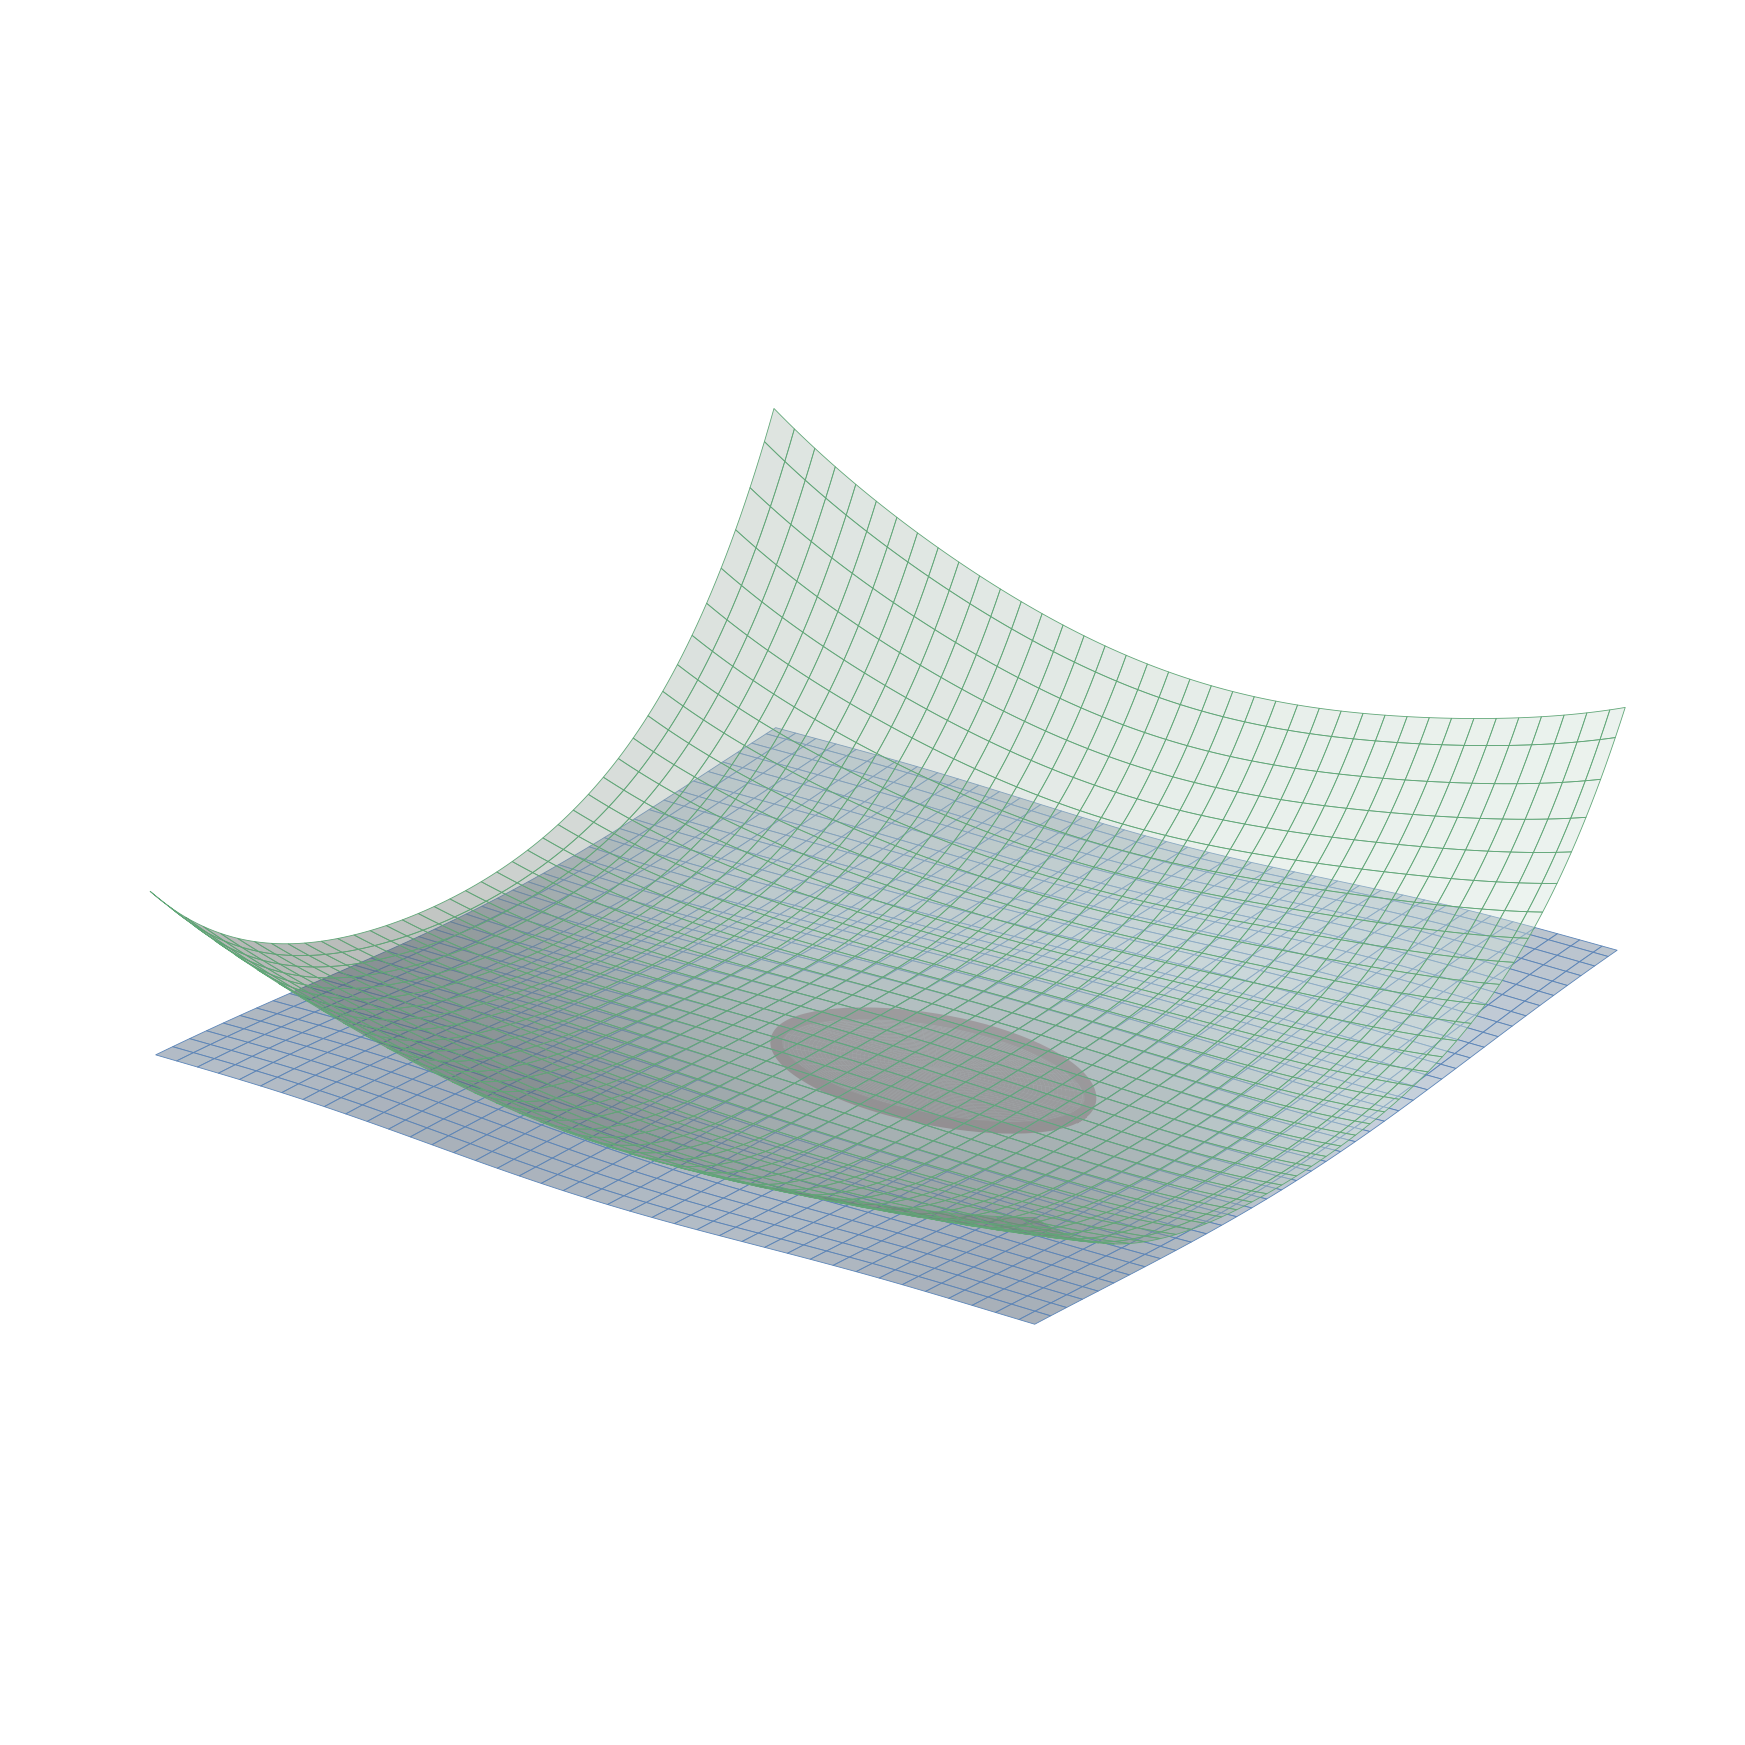
\includegraphics[width=\linewidth]{figures/calg_cmame_used/static_patch_contact_equivalence_model.png}
\end{minipage}\hfill
\begin{minipage}[t]{0.41\linewidth}
\centering
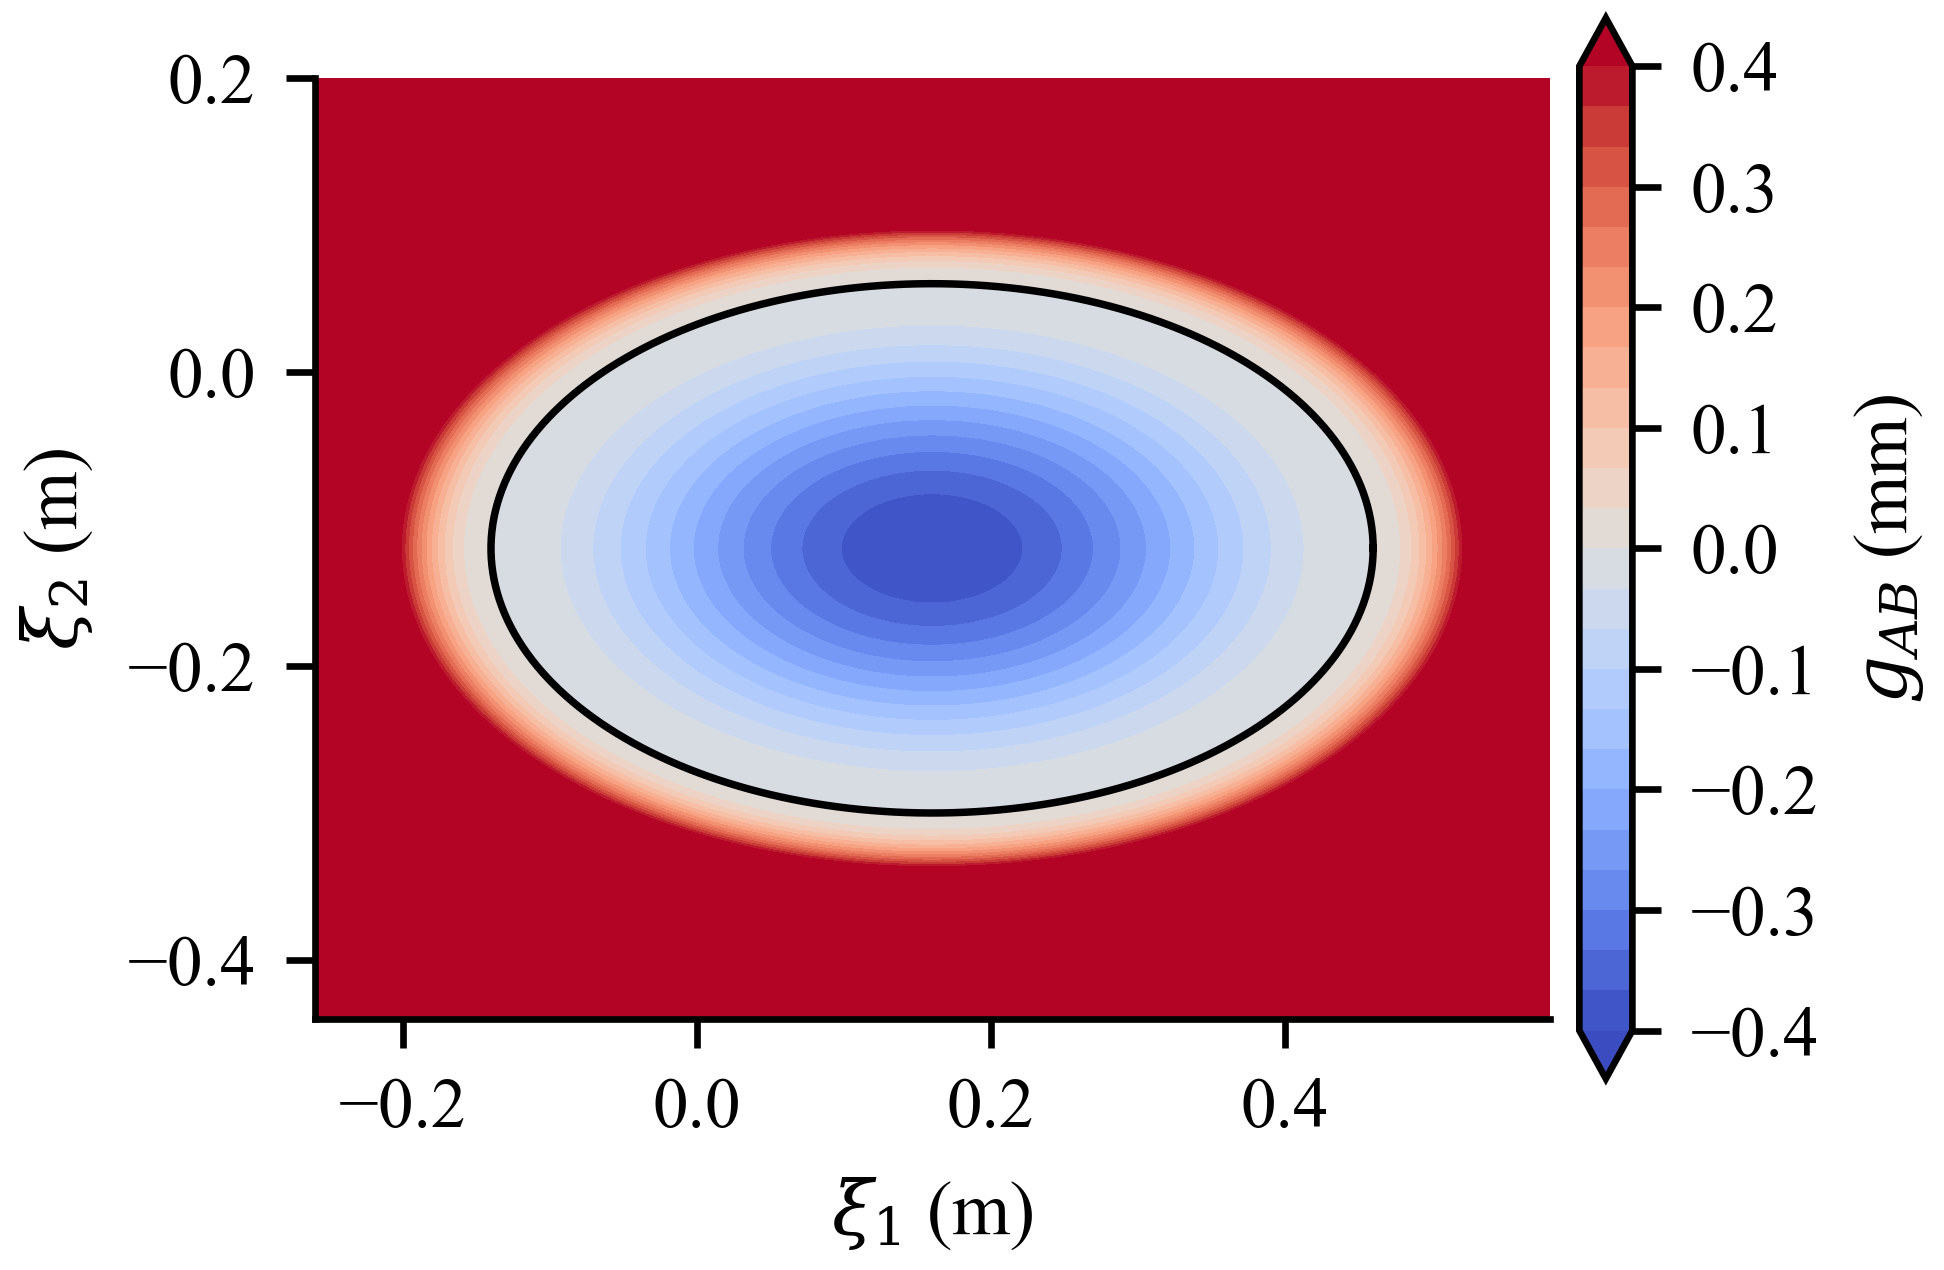
\includegraphics[width=\linewidth]{figures/calg_cmame_used/static_patch_contact_equivalence_gap_field.png}
\end{minipage}
\caption{Static patch-contact equivalence setup. The active contact patch is an ellipse embedded in two graphable, geometrically complex analytic surfaces. The right panel shows the prescribed signed graph gap in the local contact coordinates; negative values are the active compressed region.}
\label{fig:static_patch_contact_equivalence}
\end{figure}

\begin{table}[H]
\centering
\caption{Static patch-contact equivalence metrics. The reference active area, gap integral, mean gap, and normal force have analytic values; pressure center and average normal are compared with high-order quadrature.}
\label{tab:static_patch_contact_equivalence}
\begin{tabular}{l r r r}
\toprule
Quantity & Reference & \calg{} graph & Error \\
\midrule
Active area (m$^2$) & $1.696460\times10^{-1}$ & $1.696460\times10^{-1}$ & $2.78\times10^{-17}$ \\
$\int_{\Omega_c}g_{AB}\,d\xi$ (m$^3$) & $-2.261947\times10^{-5}$ & $-2.261947\times10^{-5}$ & $3.05\times10^{-20}$ \\
Mean gap (m) & $-1.333333\times10^{-4}$ & $-1.333333\times10^{-4}$ & $1.63\times10^{-19}$ \\
Normal force (N) & $4.523893\times10^{1}$ & $4.523893\times10^{1}$ & $5.68\times10^{-14}$ \\
Pressure center (m) & high-order quadrature & graph quadrature & $1.02\times10^{-15}$ \\
Mean normal angle (deg) & high-order quadrature & graph quadrature & $<10^{-12}$ \\
\bottomrule
\end{tabular}
\end{table}

Table~\ref{tab:static_patch_contact_equivalence} shows that the \calg{} graph-region quadrature reproduces the analytic patch quantities to roundoff accuracy in this controlled case. The active-band local graph certificate remains well conditioned, with minimum $N_A\cdot n_c=0.973$ and minimum $(-N_B)\cdot n_c=0.973$ over the sampled contact band. This check does not replace dynamic validation; it establishes that the local graph representation can be used as an area-contact object when the active region is integrated rather than collapsed to a representative point.

\FloatBarrier

\subsection{Analytic inclined-plane friction controls}

Before using frictional dynamics to evaluate contact geometry, we first isolate the friction law on a planar inclined surface where the exact Coulomb solution is available. Positive displacement is measured downslope. For a block of mass $m$ on a plane with angle $\theta$, the normal load is $N=mg\cos\theta$ and the downslope gravitational force is $mg\sin\theta$. A block released from rest remains stuck if
\begin{equation}
    mg\sin\theta \le \mu_s mg\cos\theta,
\end{equation}
and otherwise enters kinetic sliding with acceleration
\begin{equation}
    a = g(\sin\theta-\mu_k\cos\theta).
    \label{eq:inclined_plane_acceleration}
\end{equation}
These controls do not test geometric accuracy because the plane normal is exact for all contact modules. They test whether the implemented rigid-friction response correctly switches between static and kinetic regimes before the more demanding curved-surface comparisons.

\FloatBarrier

\begin{figure}[t]
\centering
\begin{minipage}[t]{0.32\linewidth}
\centering
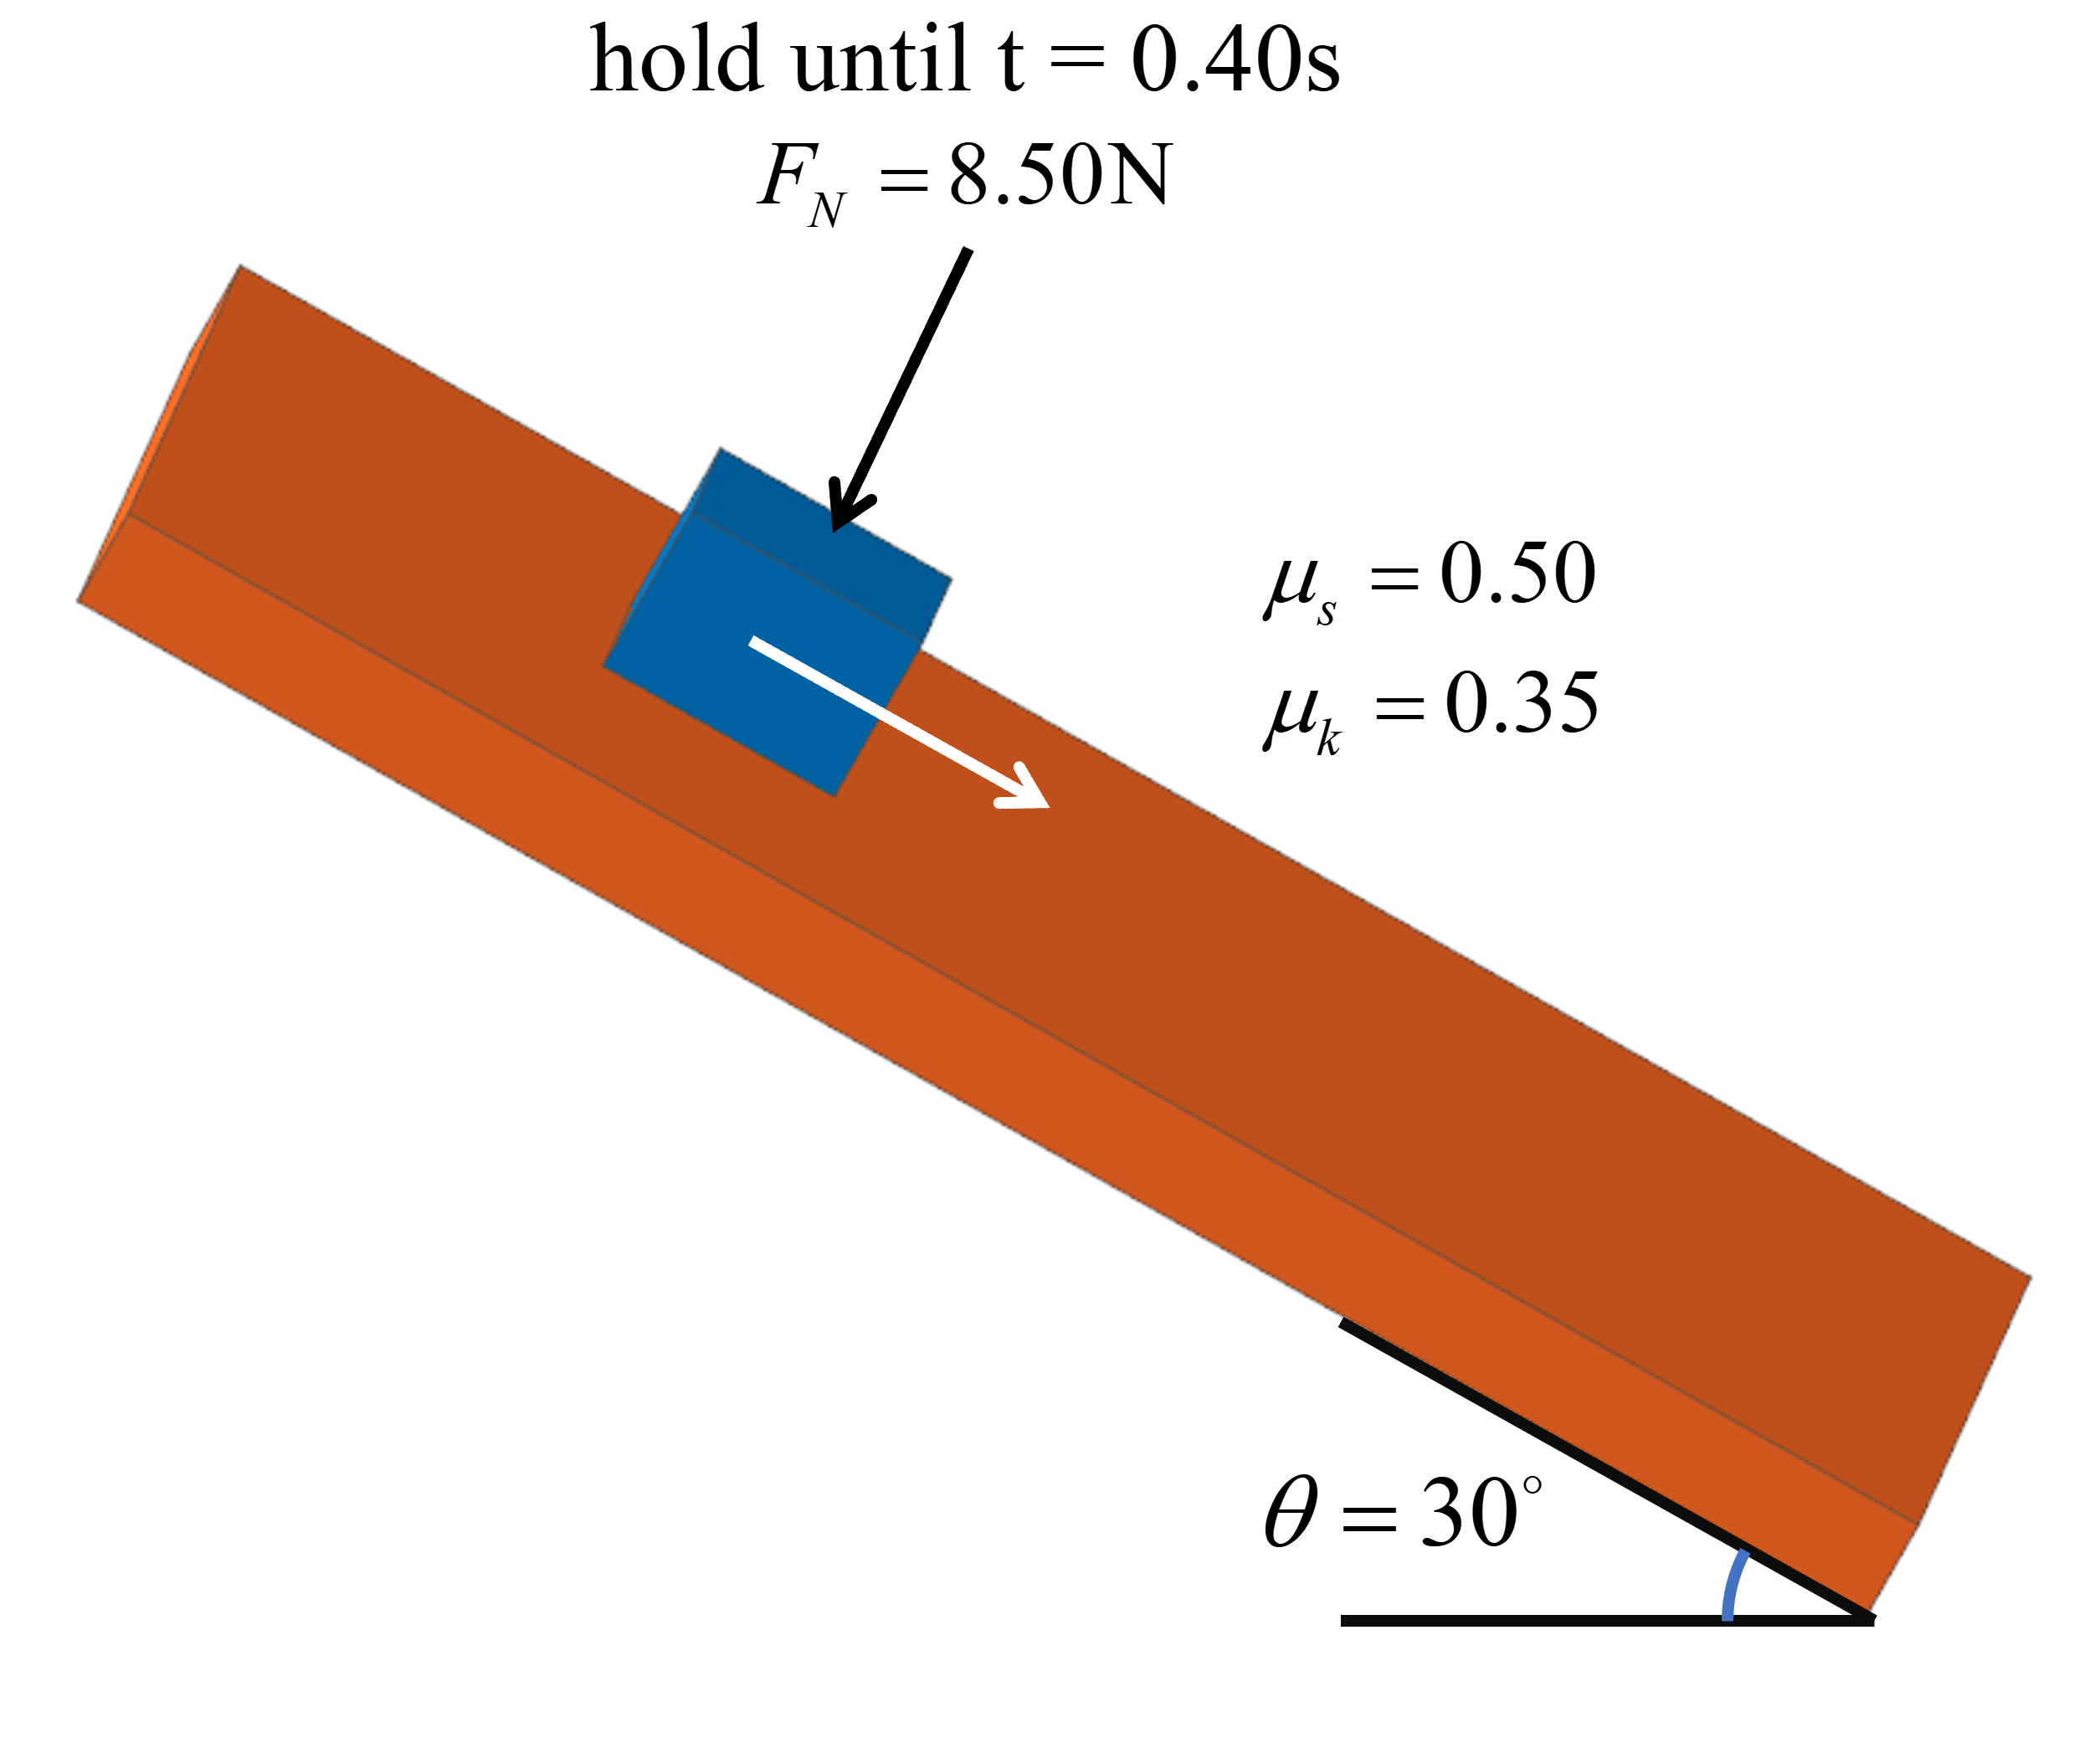
\includegraphics[width=\linewidth]{figures/calg_cmame_used/CALG_Model_friction_1.png}
\end{minipage}\hfill
\begin{minipage}[t]{0.32\linewidth}
\centering
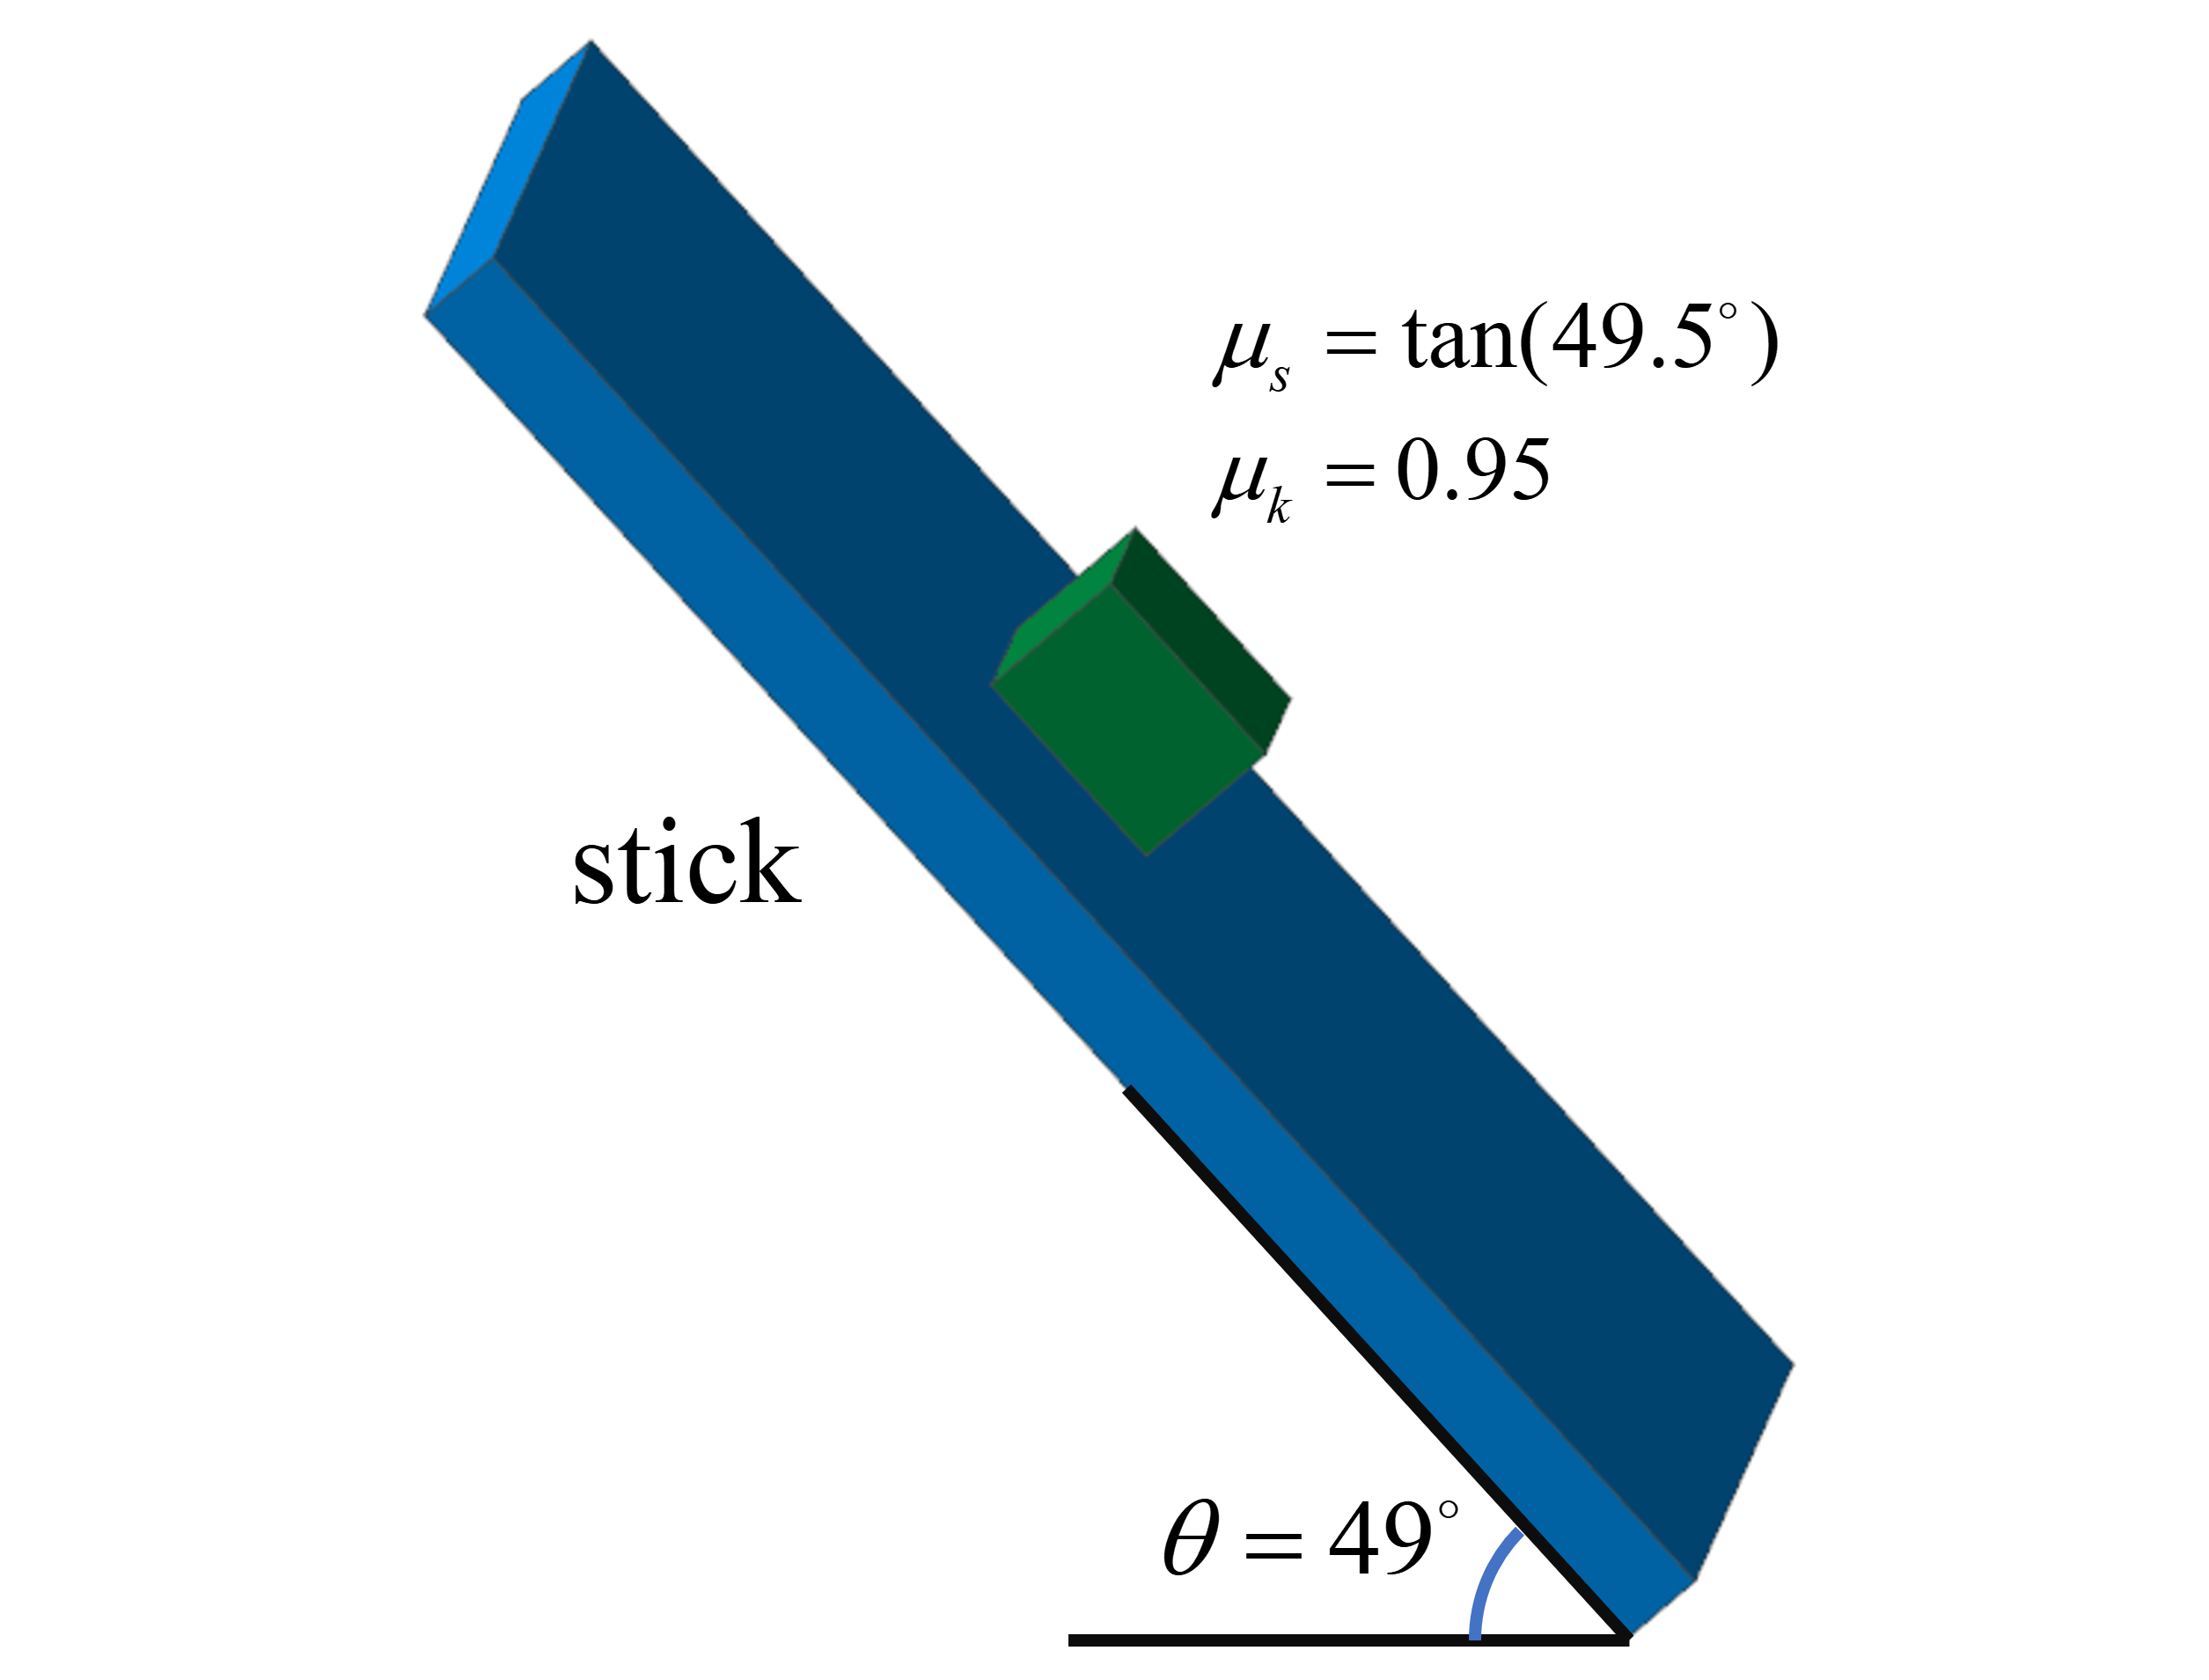
\includegraphics[width=\linewidth]{figures/calg_cmame_used/CALG_Model_friction_2.png}
\end{minipage}\hfill
\begin{minipage}[t]{0.32\linewidth}
\centering
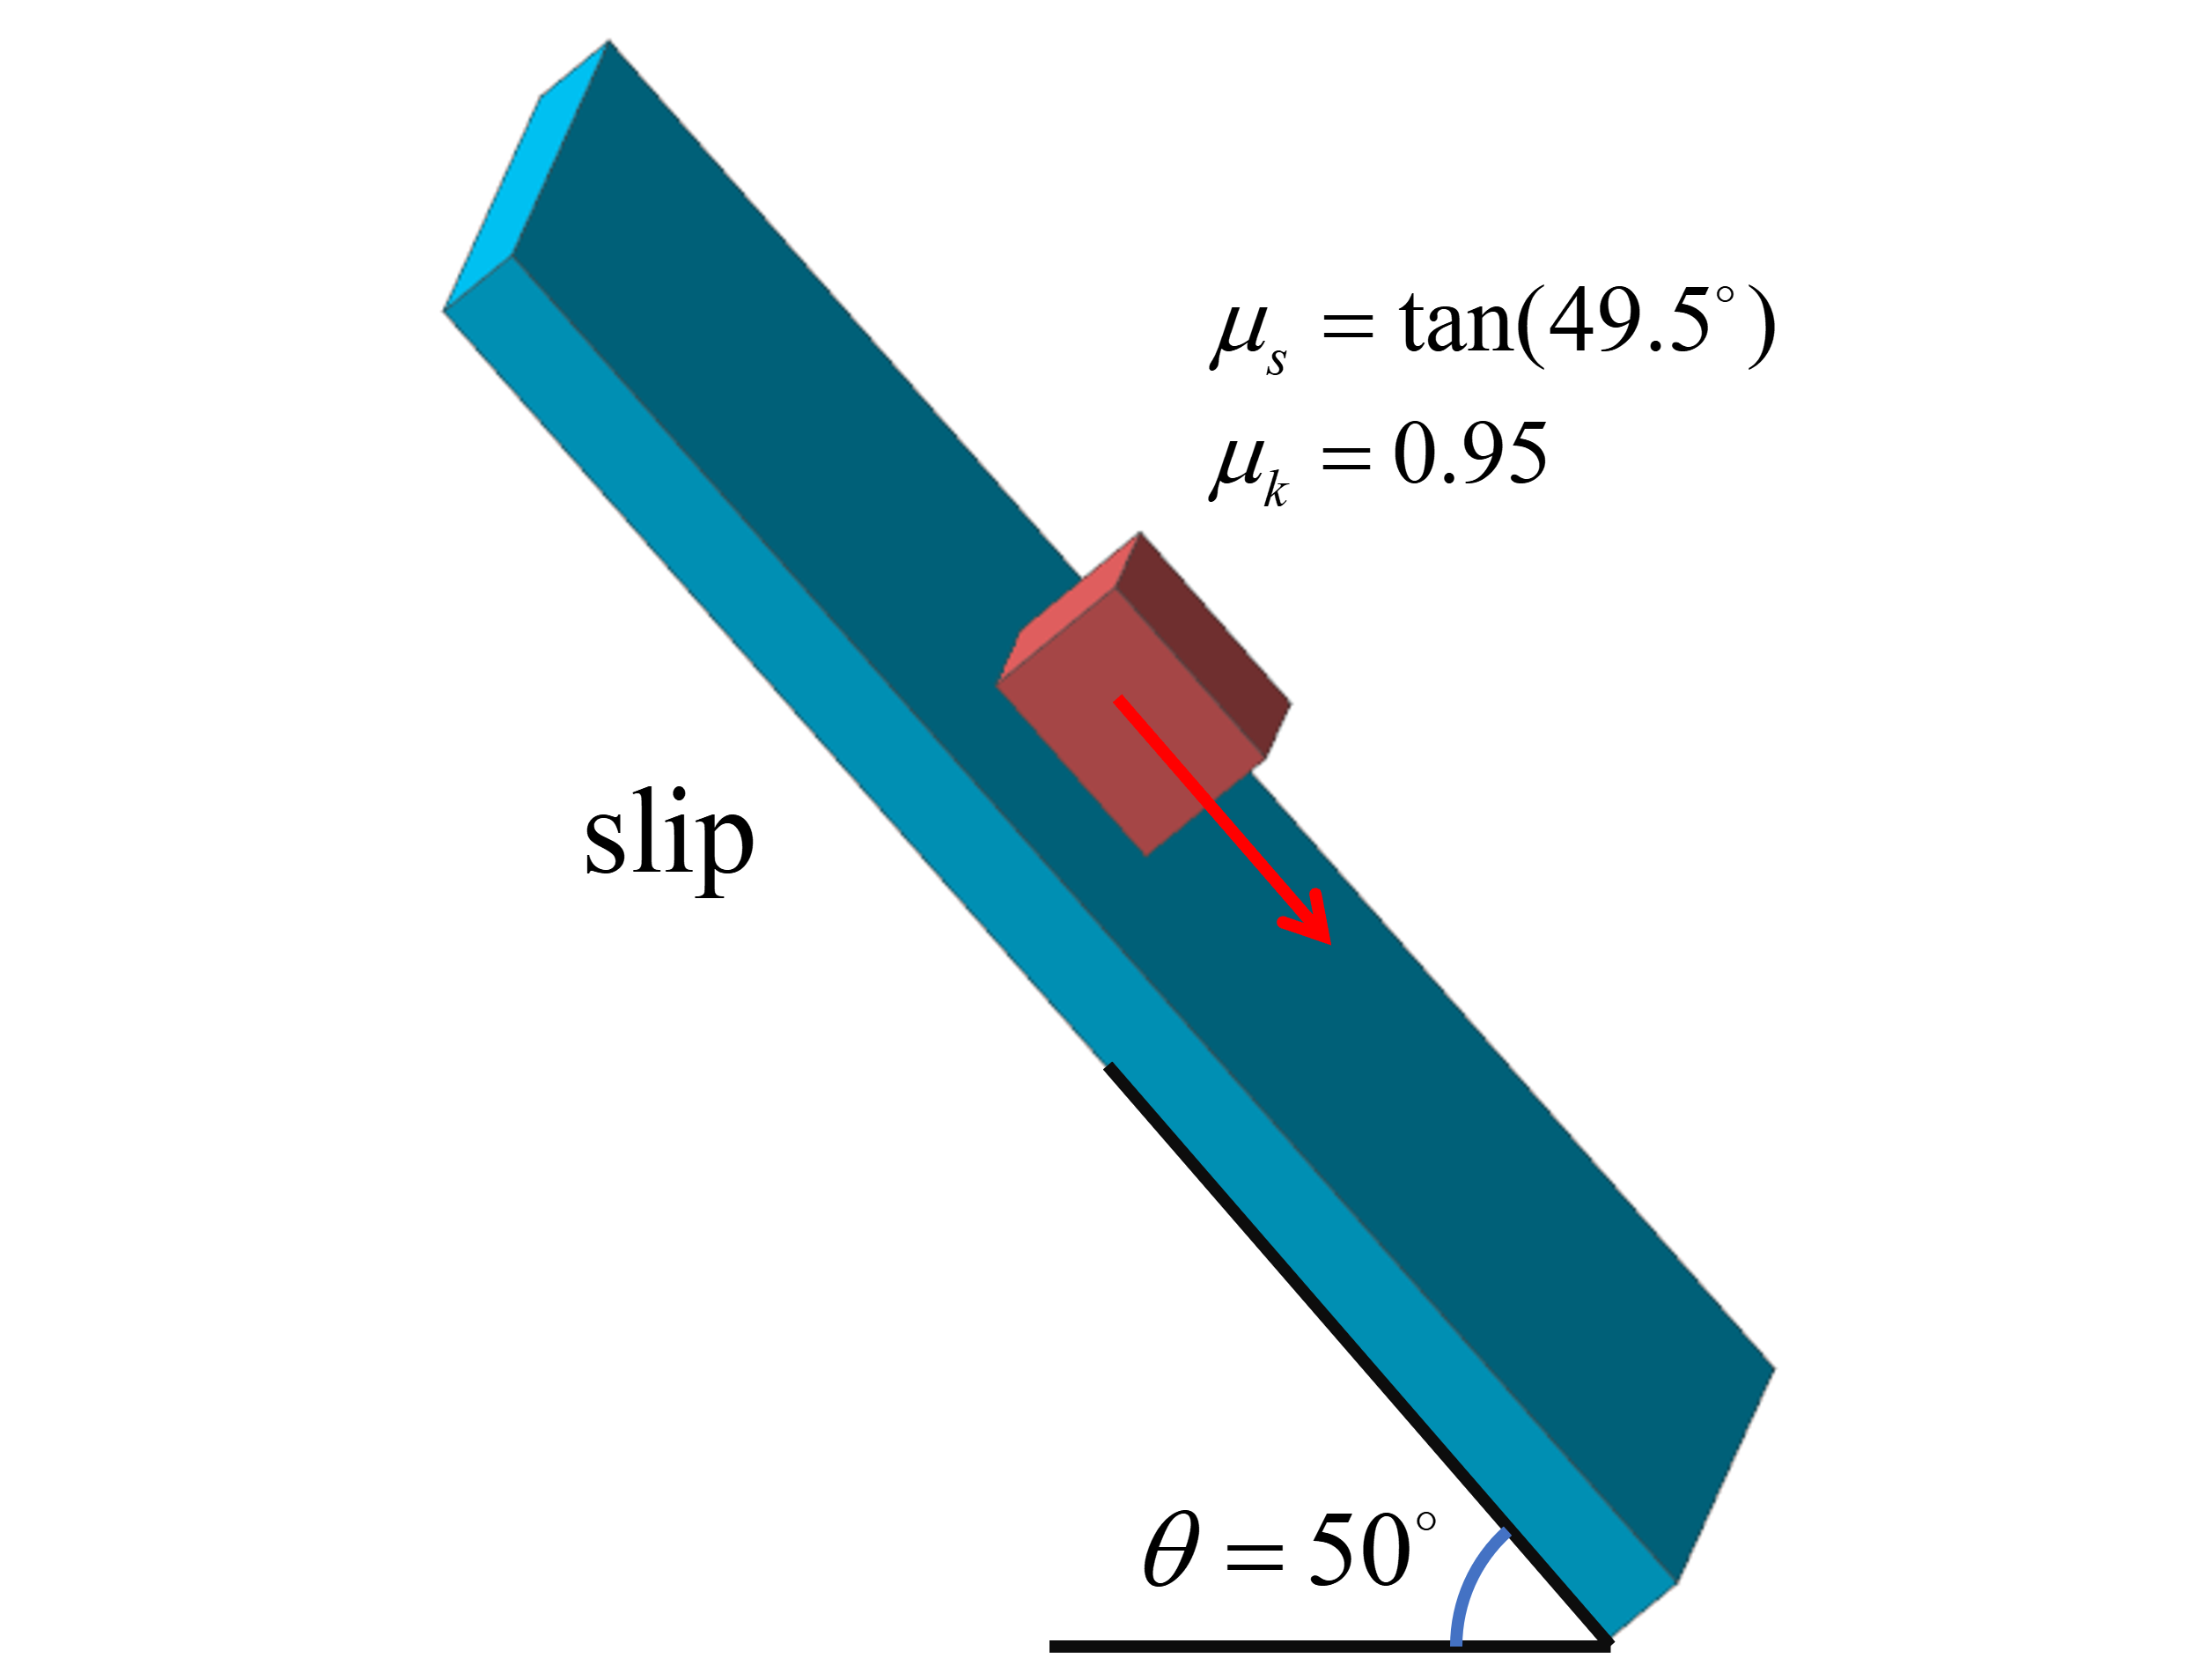
\includegraphics[width=\linewidth]{figures/calg_cmame_used/CALG_Model_friction_3.png}
\end{minipage}
\caption{Model configuration for the analytic inclined-plane controls. The three views show the $30^\circ$ release case and the two static-friction threshold cases with identical block-plane geometry. The threshold cases change the slope angle from $49^\circ$ to $50^\circ$ while keeping $\mu_s=\tan(49.5^\circ)$.}
\label{fig:inclined_friction_models}
\end{figure}

\begin{figure}[t]
\centering
\begin{minipage}[t]{0.32\linewidth}
\centering
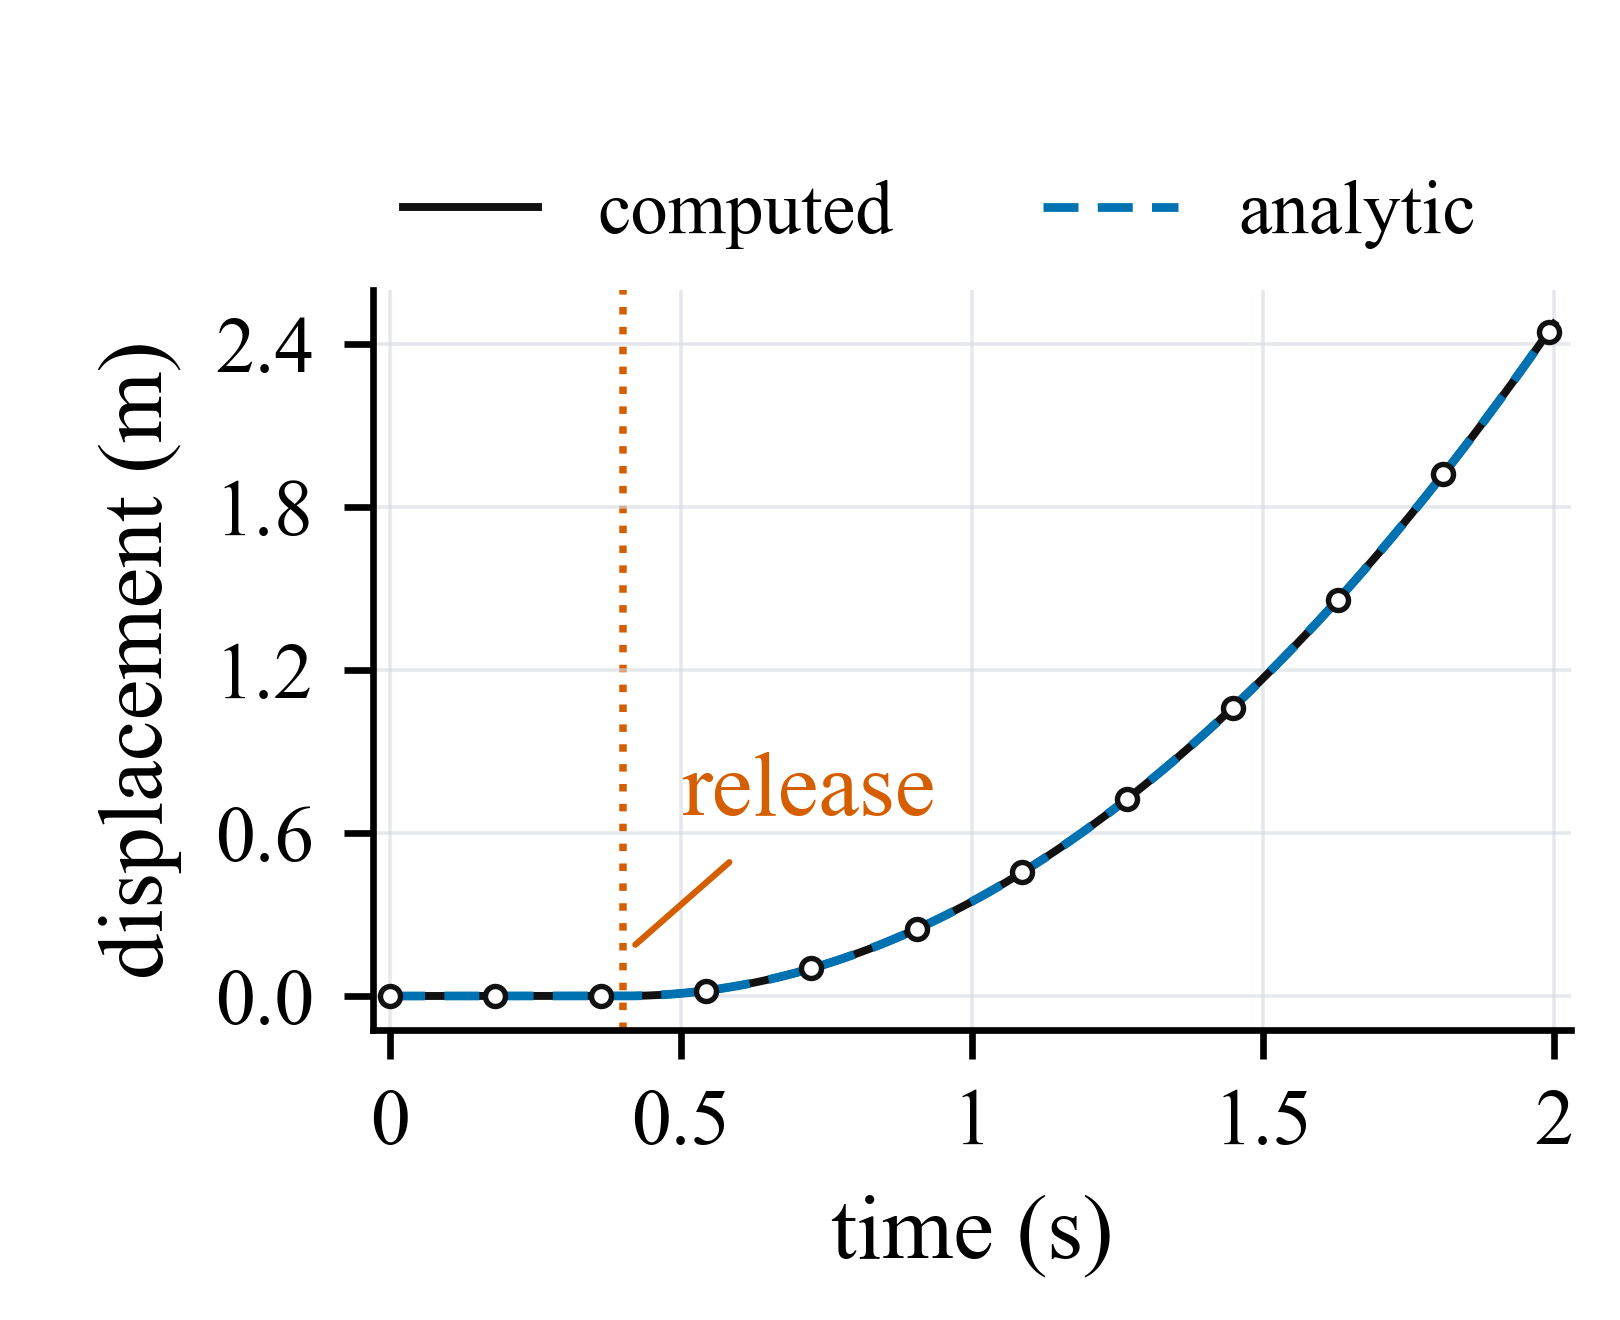
\includegraphics[width=\linewidth]{figures/calg_cmame_used/05_inclined_release_displacement.png}
\end{minipage}\hfill
\begin{minipage}[t]{0.32\linewidth}
\centering
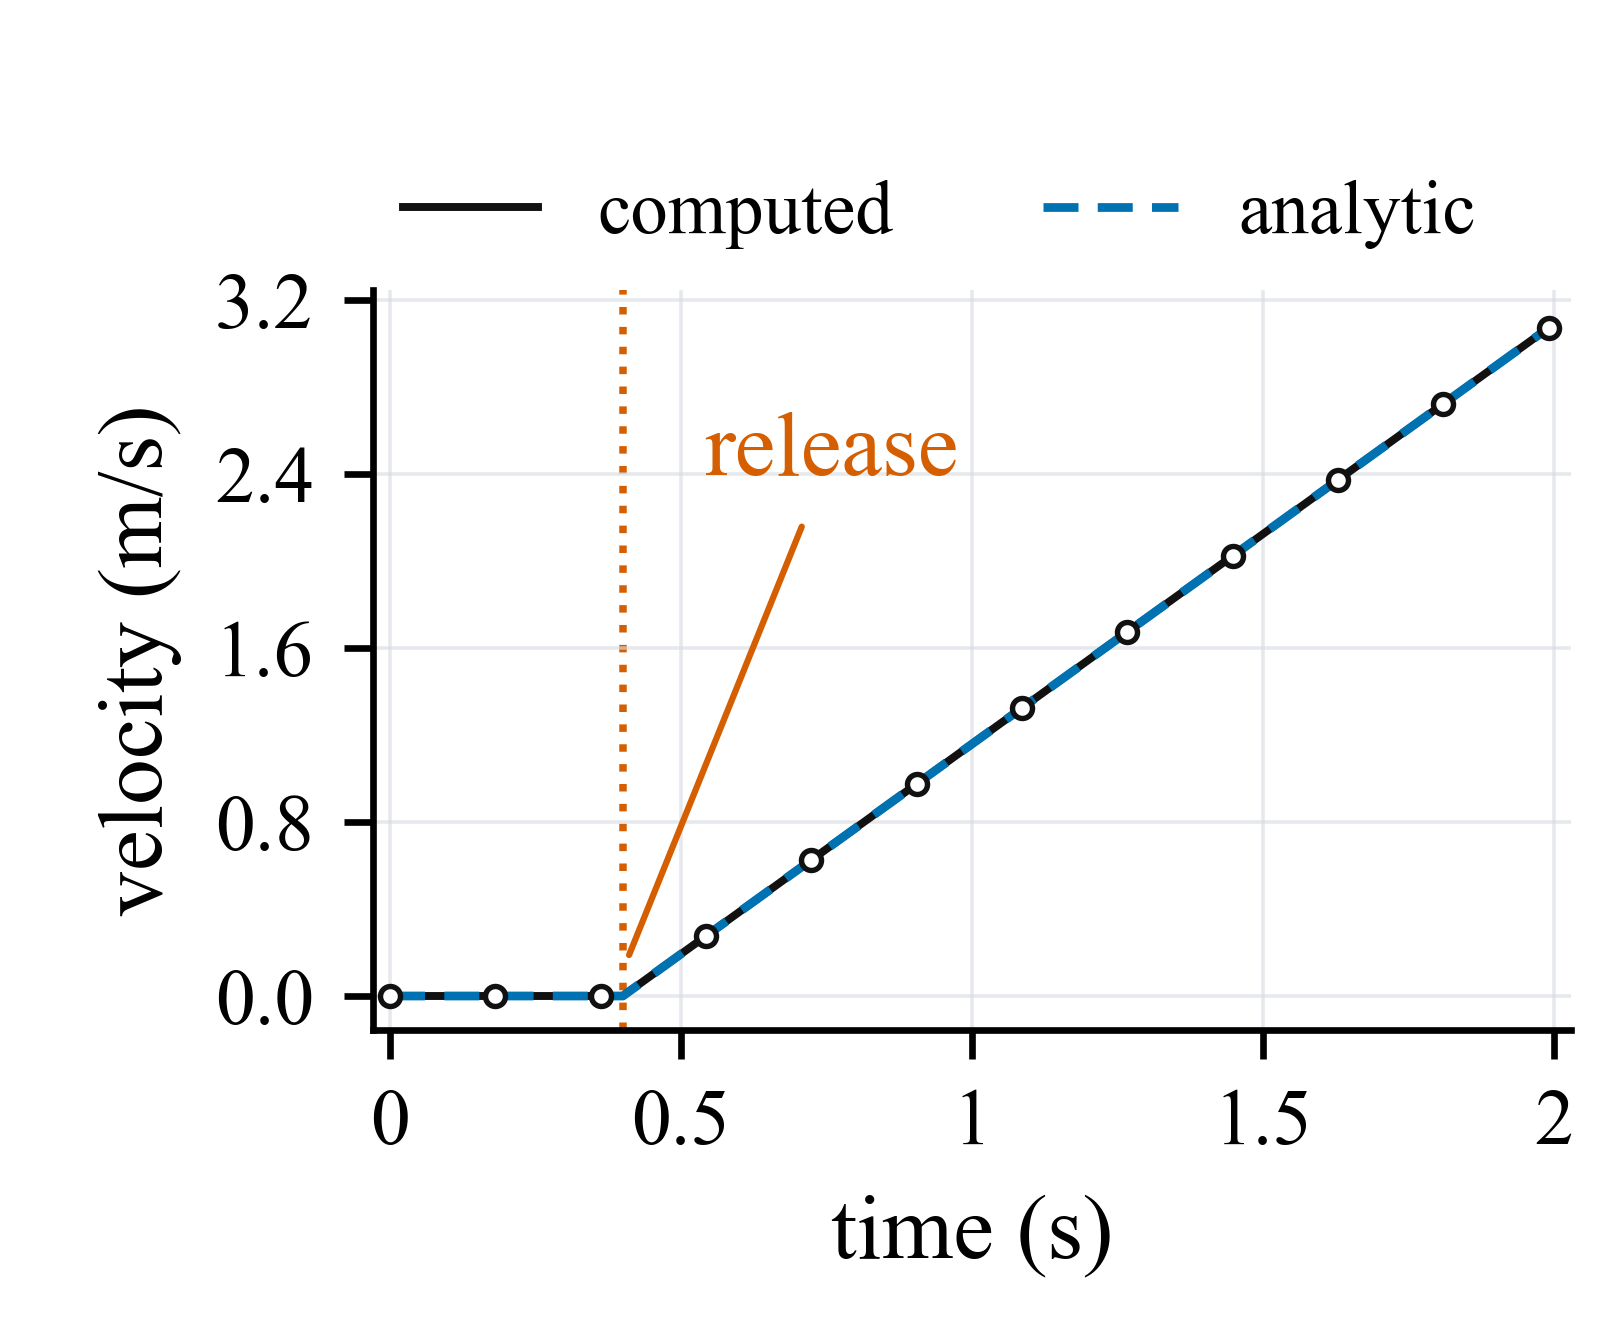
\includegraphics[width=\linewidth]{figures/calg_cmame_used/05_inclined_release_velocity.png}
\end{minipage}\hfill
\begin{minipage}[t]{0.32\linewidth}
\centering
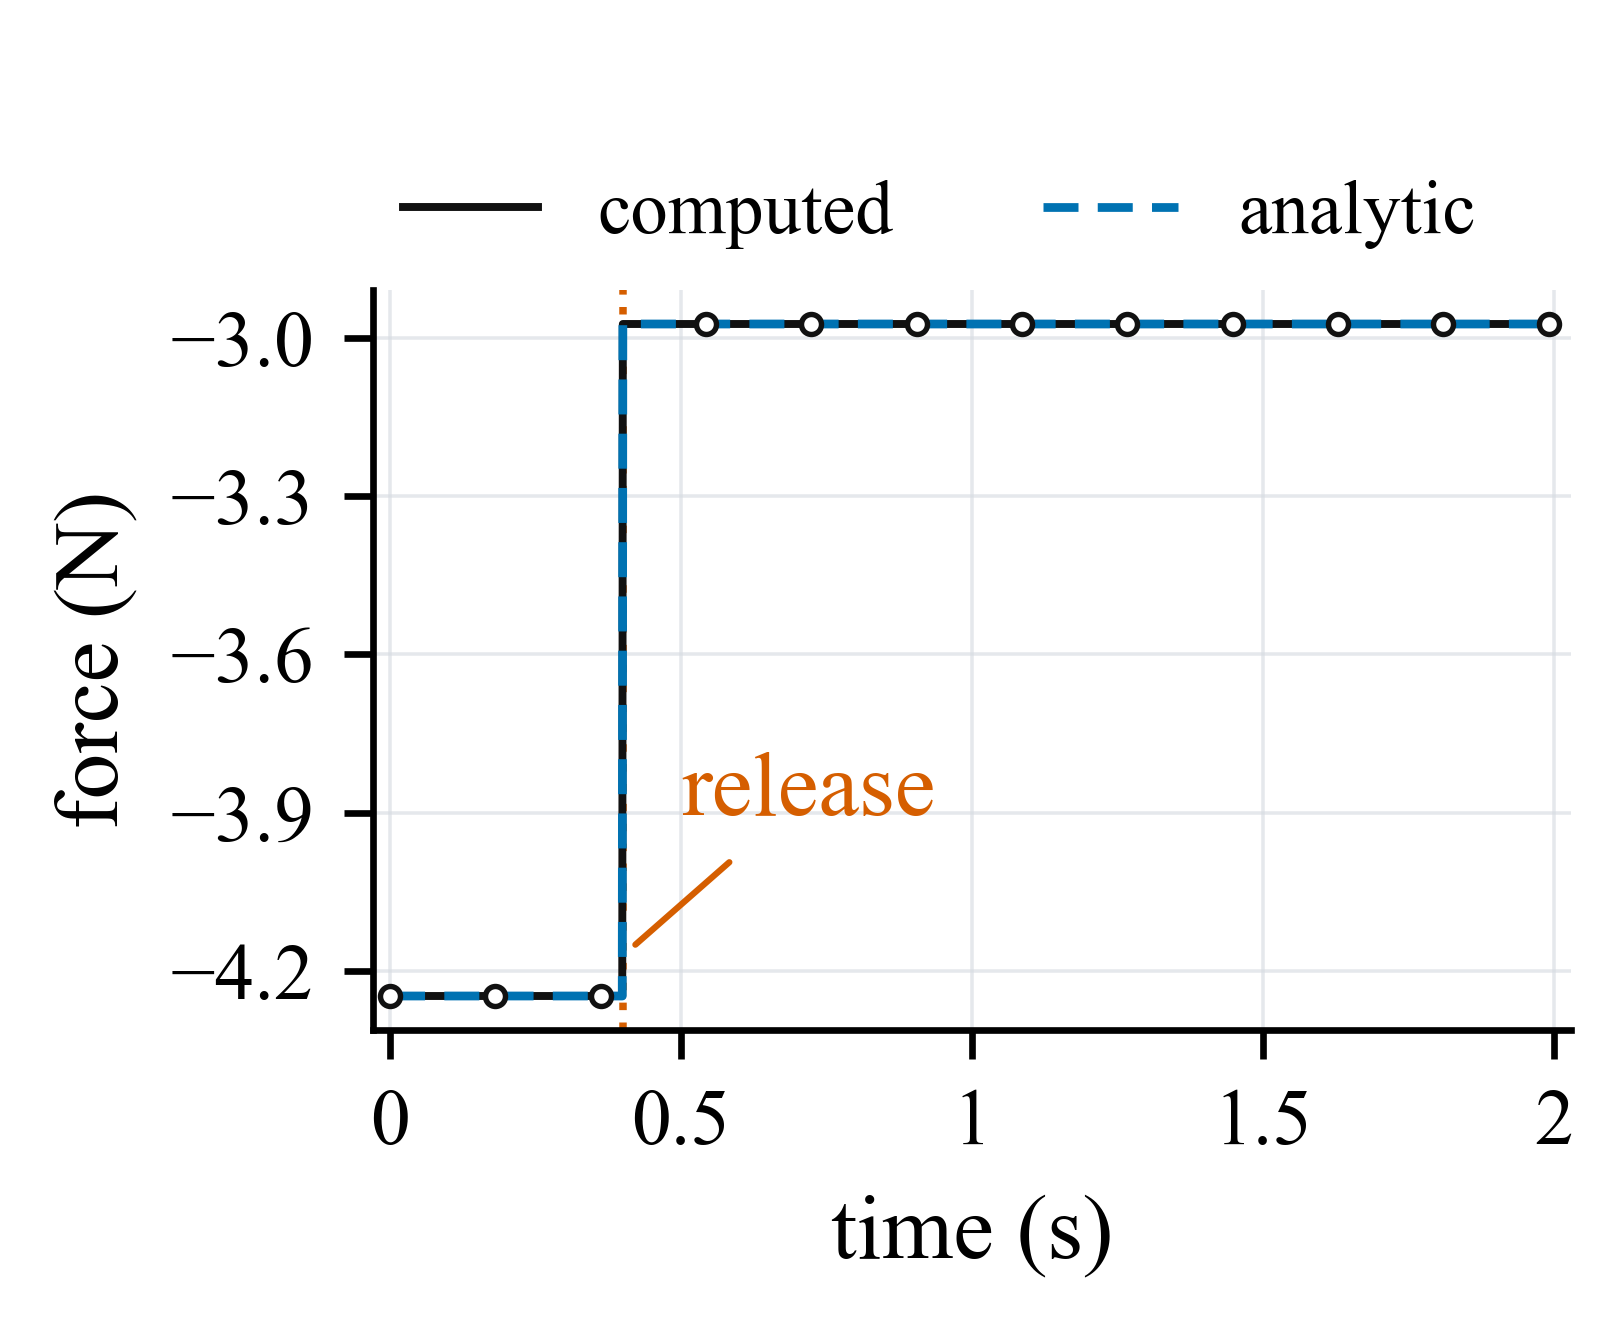
\includegraphics[width=\linewidth]{figures/calg_cmame_used/05_inclined_release_friction_force.png}
\end{minipage}
\caption{Release control on a $30^\circ$ inclined plane. The block is held until $t=0.40$ s and then released; because the static capacity is exceeded, it switches to kinetic sliding and follows Eq.~\eqref{eq:inclined_plane_acceleration}. The black computed curve and blue dashed analytic curve are plotted separately, with markers on the computed samples to keep the coincident curves distinguishable.}
\label{fig:inclined_release_controls}
\end{figure}

\begin{table}[t]
\centering
\caption{Analytic inclined-plane friction controls. Static margin is $\mu_smg\cos\theta-mg\sin\theta$; positive values indicate sticking is admissible.}
\label{tab:inclined_friction_controls}
{\setlength{\tabcolsep}{4pt}
\begin{tabular}{l r c r c r r}
\toprule
Case & $\theta$ (deg) & $(\mu_s,\mu_k)$ & Margin (N) & Outcome & $a$ (m/s$^2$) & $s(T)$ (m) \\
\midrule
Release & 30.0 & (0.500, 0.350) & -0.657 & slip & 1.932 & 2.472 \\
Threshold 49 deg & 49.0 & (1.171, 0.950) & 0.132 & stick & 0 & 0 \\
Threshold 50 deg & 50.0 & (1.171, 0.950) & -0.132 & slip & 1.524 & 0.762 \\
\bottomrule
\end{tabular}
}
\end{table}

\FloatBarrier

\subsection{Engineering scenes and compared geometry modules}

The dynamic contact-geometry comparison isolates the contact-geometry module while keeping the rigid-body update fixed. Linear-triangle BVH uses the piecewise-linear triangle mesh and face normals. PN-triangle BVH evaluates a fixed-tessellation PN-triangle approximation constructed from the same input geometry. \calg{}--SDF uses the contact-aligned local graph detector, certified fallback hierarchy, and configuration-space signed-distance response layer to return the contact point, signed gap, contact normal, and tangential frame used by the same regularized Coulomb update.

\FloatBarrier

\begin{figure}[t]
\centering
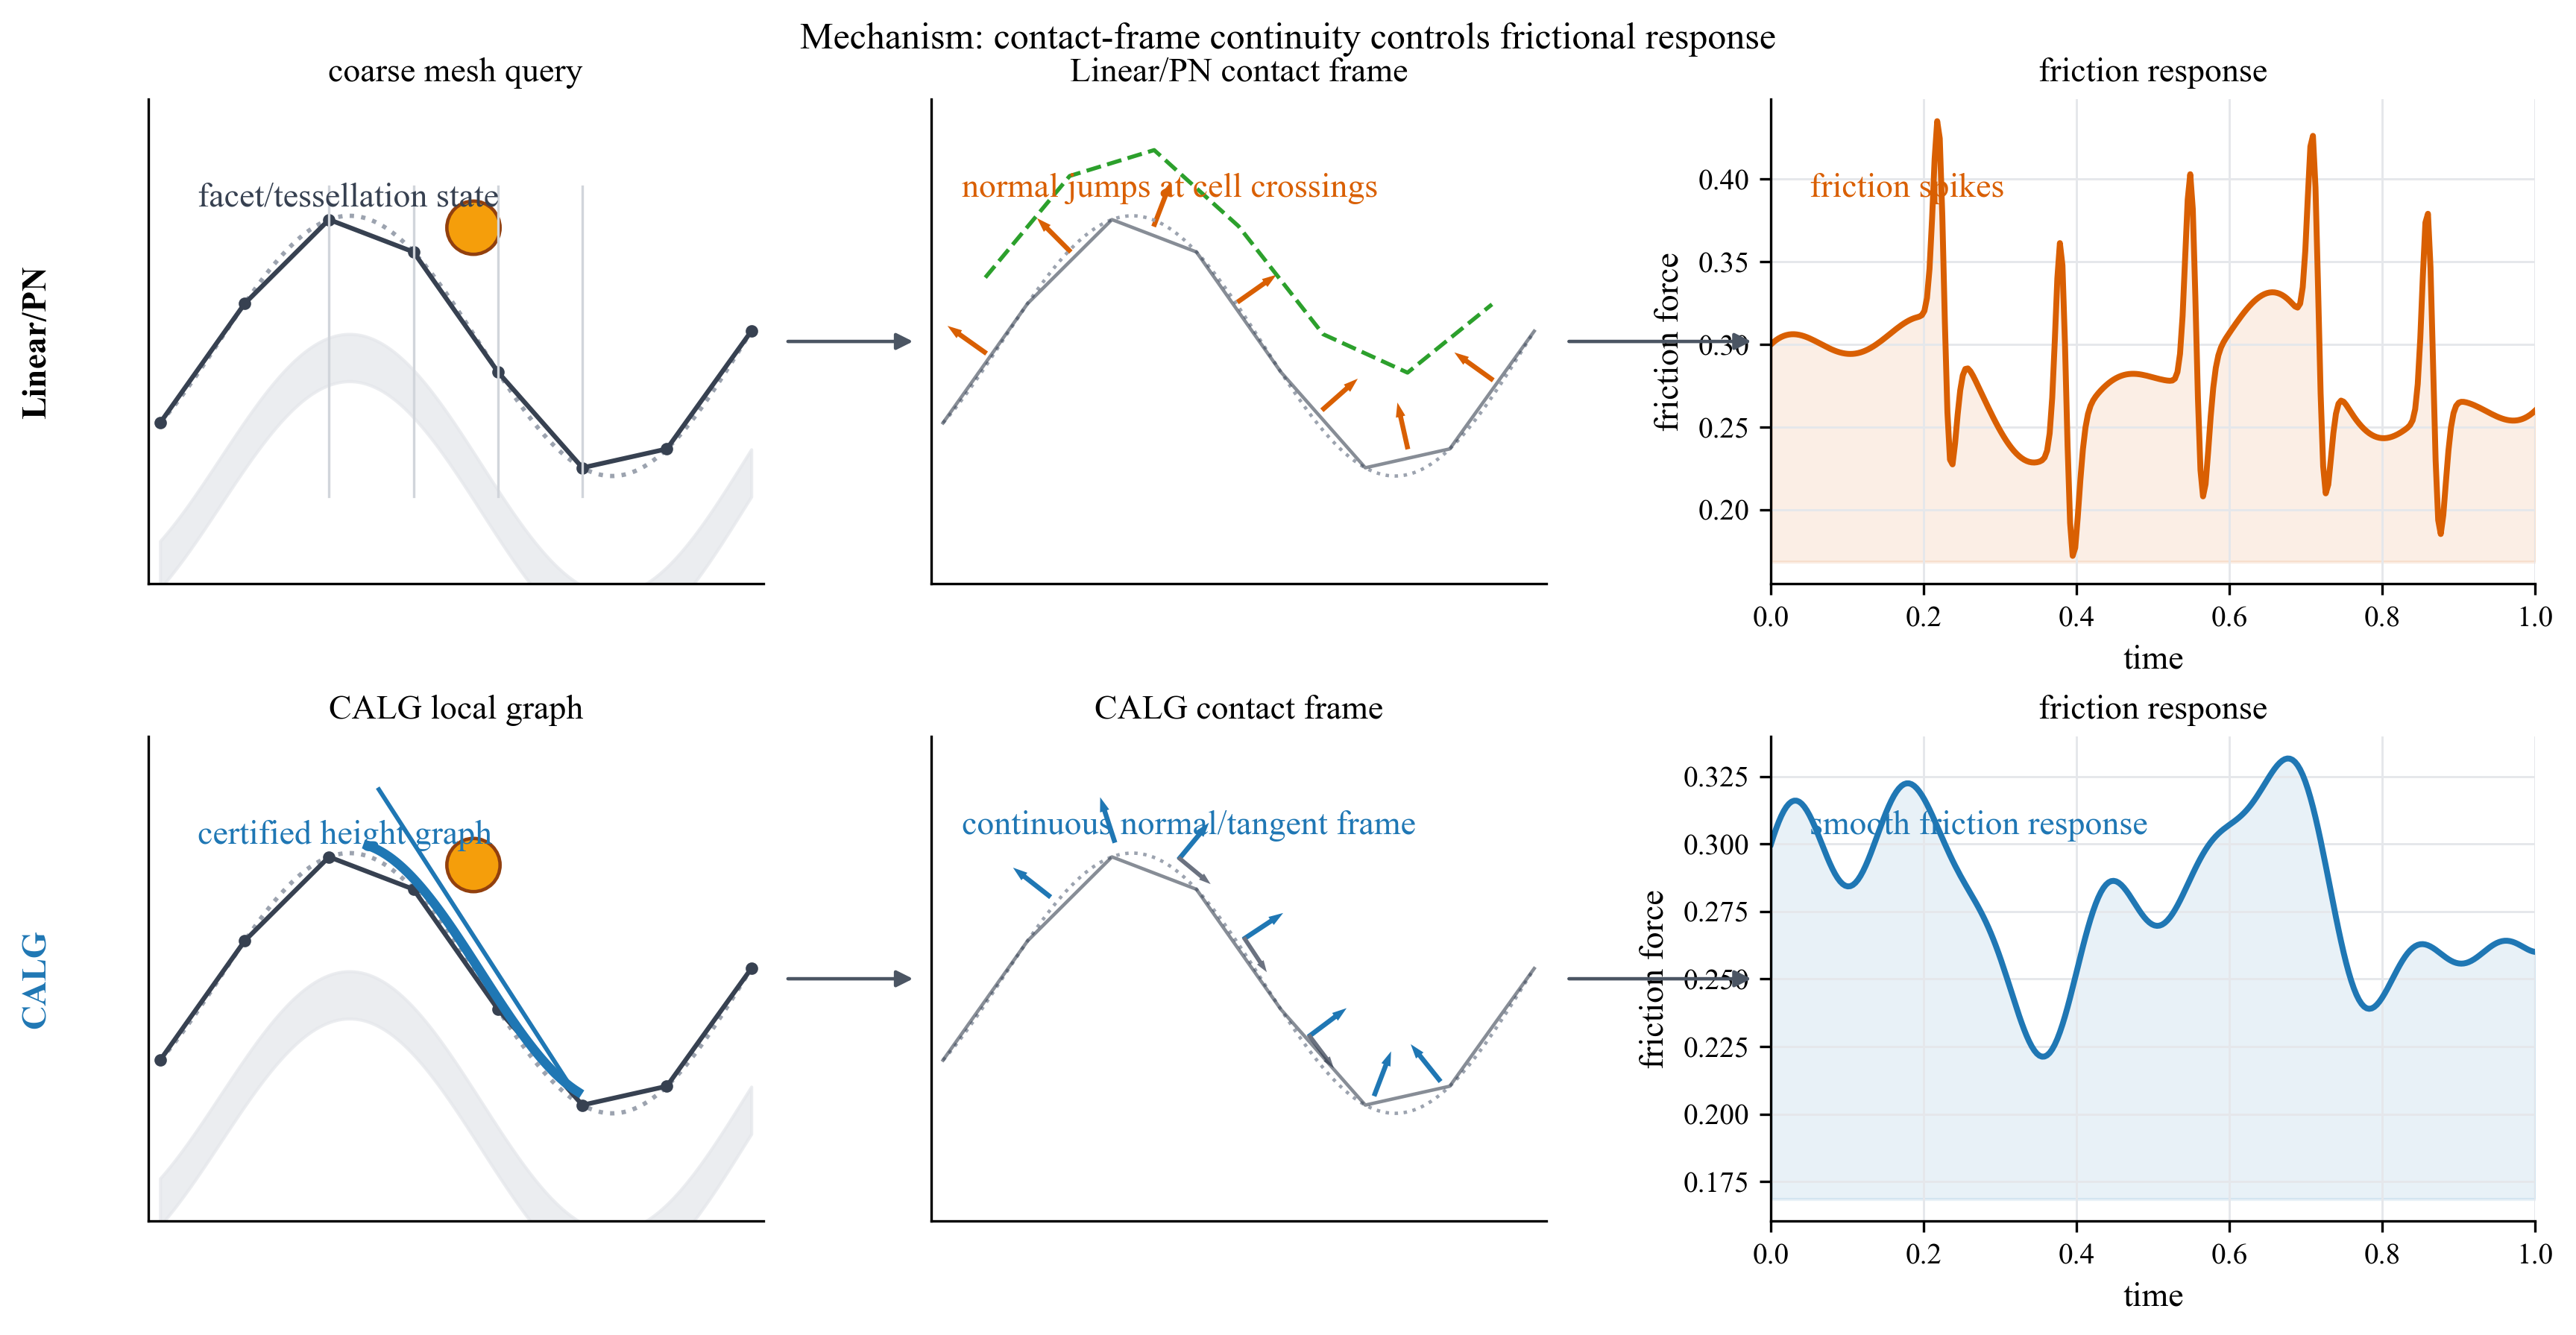
\includegraphics[width=\linewidth]{figures/calg_cmame_used/01_mechanism_story.png}
\caption{Mechanism-level comparison between facet-based contact-geometry modules and \calg{}--SDF. Linear-triangle BVH and fixed-tessellation PN-triangle BVH inherit cell-crossing changes in the contact normal or tangent frame, which can enter the regularized Coulomb response as force spikes. \calg{} instead certifies a contact-aligned local height graph and returns a smooth normal and tangent frame, producing a smoother friction response in the same rigid-body update.}
\label{fig:mechanism_story}
\end{figure}

\begin{figure}[t]
\centering
\begin{minipage}[t]{0.32\linewidth}
\centering
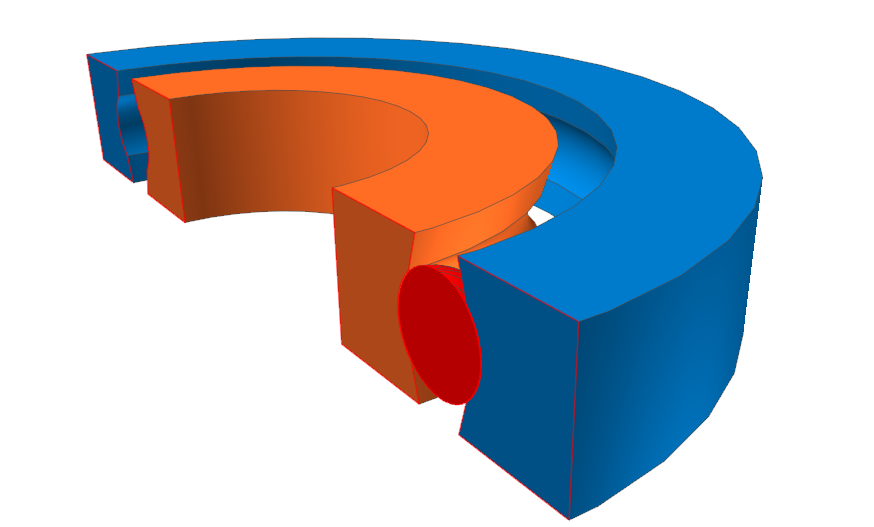
\includegraphics[width=\linewidth]{figures/calg_cmame_used/CALG_Model_bearing_raceway_1.png}
\end{minipage}\hfill
\begin{minipage}[t]{0.32\linewidth}
\centering
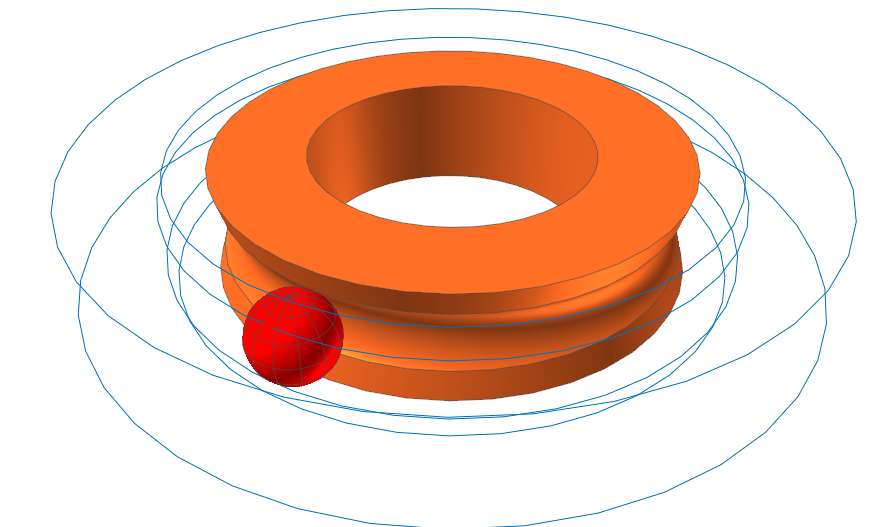
\includegraphics[width=\linewidth]{figures/calg_cmame_used/CALG_Model_bearing_raceway_2.png}
\end{minipage}\hfill
\begin{minipage}[t]{0.32\linewidth}
\centering
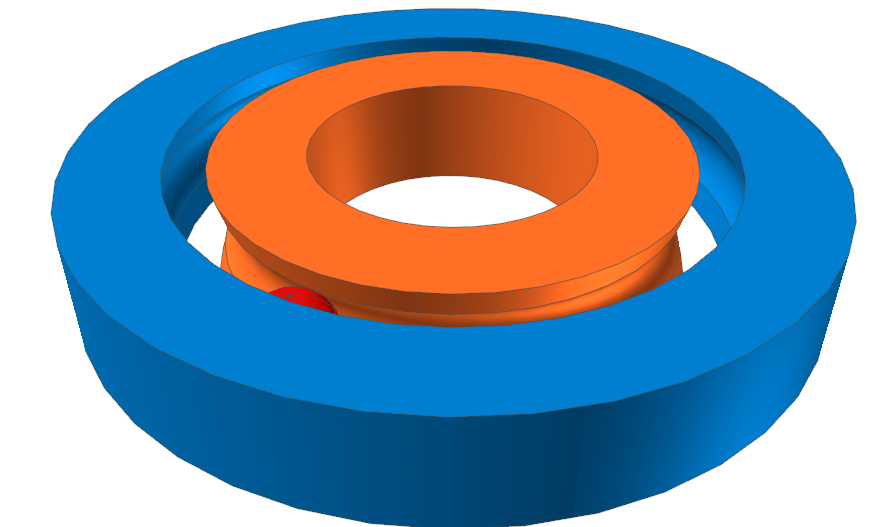
\includegraphics[width=\linewidth]{figures/calg_cmame_used/CALG_Model_bearing_raceway_3.png}
\end{minipage}
\caption{Model configuration for the Bearing raceway scene. The three views show the imported raceway geometry and rolling element configuration used by Recurdyn, Chrono, and \calg{}.}
\label{fig:model_bearing}
\end{figure}

\begin{figure}[t]
\centering
\begin{minipage}[t]{0.49\linewidth}
\centering
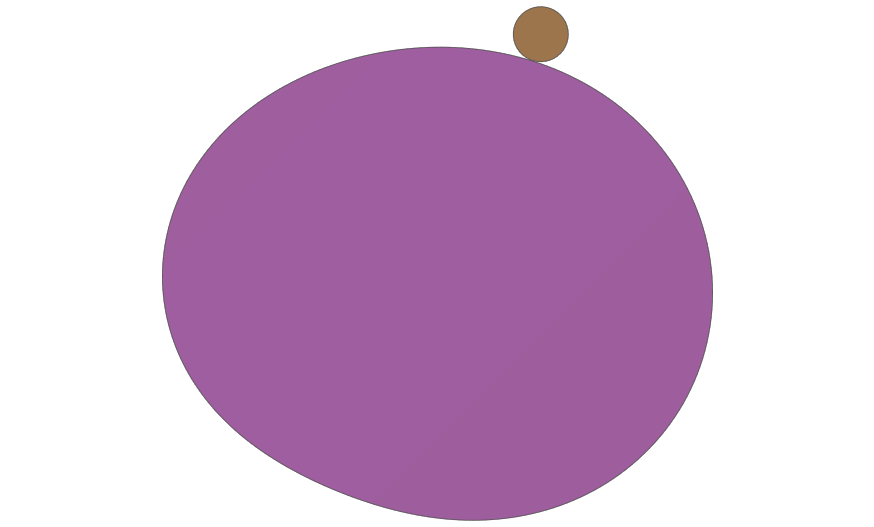
\includegraphics[width=\linewidth]{figures/calg_cmame_used/CALG_Model_cam_1.png}
\end{minipage}\hfill
\begin{minipage}[t]{0.49\linewidth}
\centering
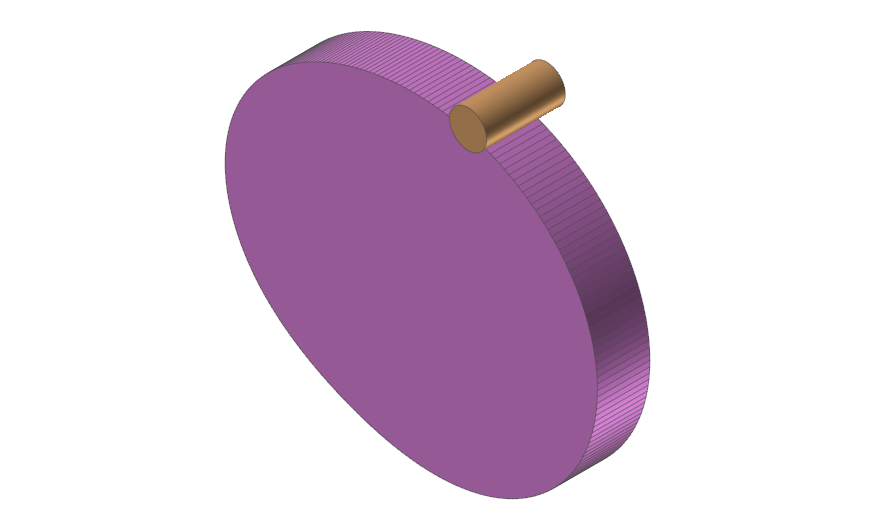
\includegraphics[width=\linewidth]{figures/calg_cmame_used/CALG_Model_cam_2.png}
\end{minipage}
\caption{Model configuration for the Cam-roller follower scene. The two views show the non-circular cam profile and roller follower geometry that produces sliding and rolling contact over a faceted collision representation.}
\label{fig:model_cam}
\end{figure}

\begin{figure}[t]
\centering
\begin{minipage}[t]{0.32\linewidth}
\centering
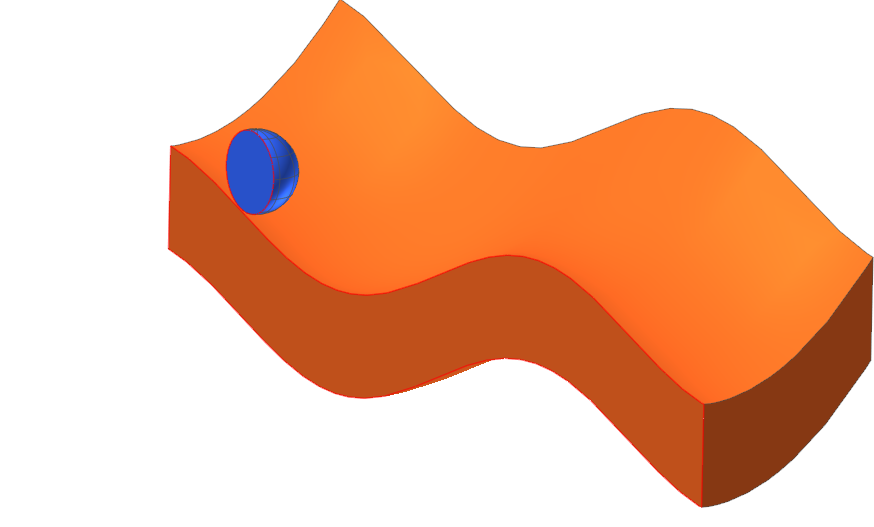
\includegraphics[width=\linewidth]{figures/calg_cmame_used/CALG_Model_guide_slot_0.png}
\end{minipage}\hfill
\begin{minipage}[t]{0.32\linewidth}
\centering
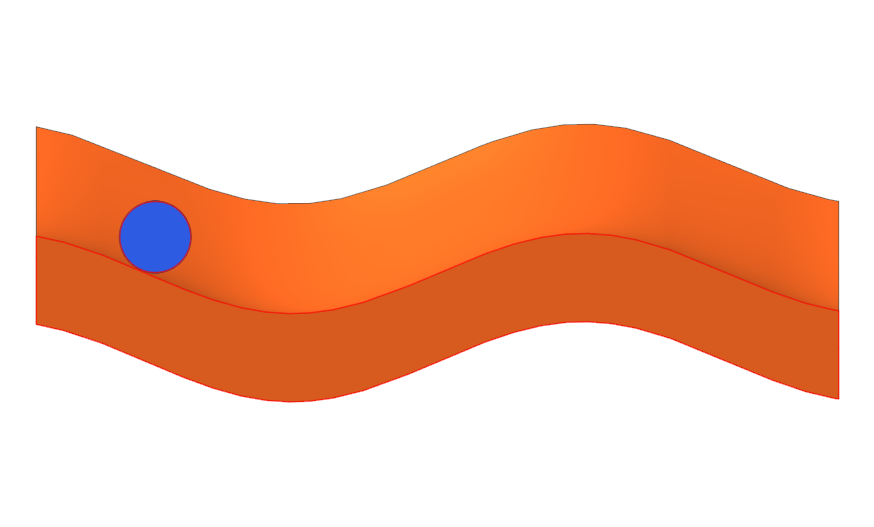
\includegraphics[width=\linewidth]{figures/calg_cmame_used/CALG_Model_guide_slot_1.png}
\end{minipage}\hfill
\begin{minipage}[t]{0.32\linewidth}
\centering
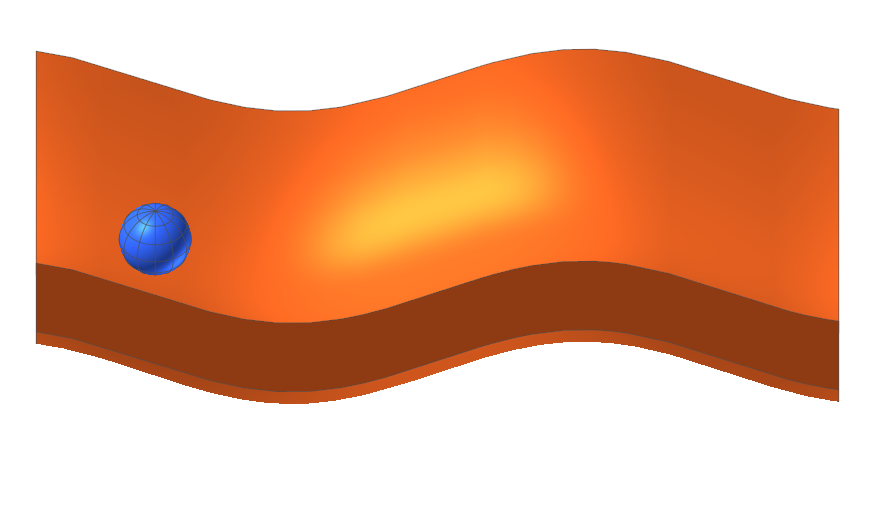
\includegraphics[width=\linewidth]{figures/calg_cmame_used/CALG_Model_guide_slot_3.png}
\end{minipage}
\caption{Model configuration for the Guide slot scene. The three views show the slot path, moving contact body, and contact geometry used by Recurdyn, Chrono, and \calg{}.}
\label{fig:model_guide}
\end{figure}

\begin{figure}[t]
\centering
\begin{minipage}[t]{0.32\linewidth}
\centering
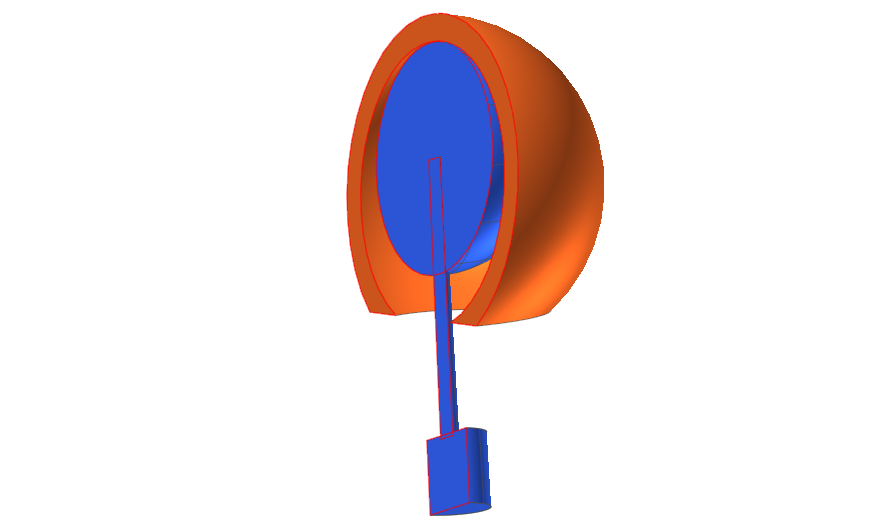
\includegraphics[width=\linewidth]{figures/calg_cmame_used/CALG_Model_ball_joint_pendulum_1.png}
\end{minipage}\hfill
\begin{minipage}[t]{0.32\linewidth}
\centering
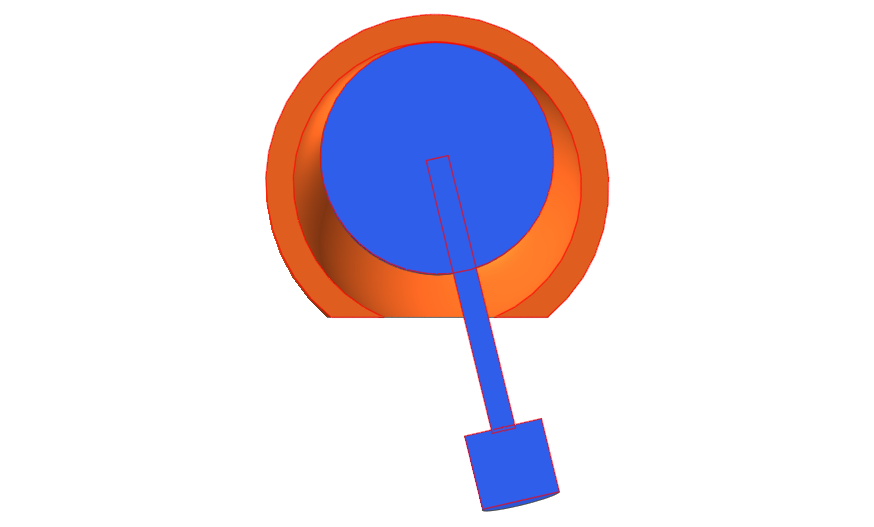
\includegraphics[width=\linewidth]{figures/calg_cmame_used/CALG_Model_ball_joint_pendulum_2.png}
\end{minipage}\hfill
\begin{minipage}[t]{0.32\linewidth}
\centering
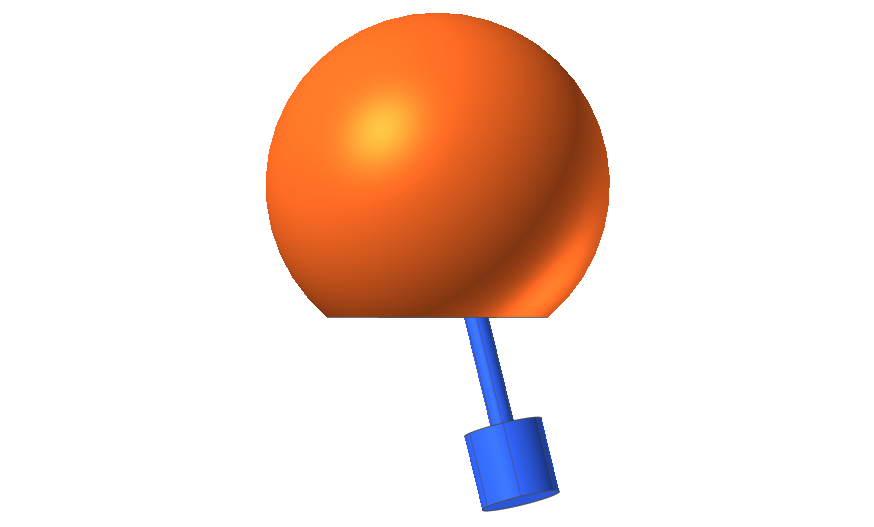
\includegraphics[width=\linewidth]{figures/calg_cmame_used/CALG_Model_ball_joint_pendulum_3.png}
\end{minipage}
\caption{Model configuration for the Ball-and-socket pendulum scene. The three views show the socket, moving contact ball, and attached pendulum body used by Recurdyn, Chrono, and \calg{}.}
\label{fig:model_ball_joint}
\end{figure}

The four scenes, Bearing raceway, Cam-roller follower, Guide slot, and Ball-and-socket pendulum, cover common rigid contact mechanisms in which friction is strongly coupled to contact-normal quality. The contact point crosses multiple surface cells in each scene, so a facet-based contact-geometry module changes the normal and tangential basis as a function of mesh topology rather than only physical geometry. The executable parameters are stated in the relevant comparison and validation paragraphs below, and the same values are stored with the generated artifacts in the reproducibility package.

\FloatBarrier

\subsection{Dynamic friction comparison against Linear-triangle BVH and PN-triangle BVH}

The main dynamic comparison runs the same rigid-body friction update with the three contact-geometry modules. All four dynamic contact-geometry comparison scenes are run for $0.8$ s with 801 stored frames and timestep $\Delta t=1.0\times10^{-3}$ s. The scene-specific rigid-body and contact parameters are fixed across Linear-triangle BVH, PN-triangle BVH, and \calg{}. The Bearing raceway scene uses a sphere of radius $0.075$ m and mass $0.65$ kg over a coarse contact mesh with $n=7$, initial velocity $(0.62,-0.08,0)$ m/s, $\mu=0.36$, detector distance $\hat d=0.065$ m, $k_n/c_n=2550/36$, and $k_t/c_t=165/0.6$. The Cam-roller follower scene uses radius $0.085$ m, mass $0.80$ kg, mesh $n=7$, initial velocity $(0.70,0.18,0)$ m/s, $\mu=0.40$, $\hat d=0.070$ m, $k_n/c_n=2800/42$, and $k_t/c_t=185/0.7$. The Guide slot scene uses radius $0.090$ m, mass $0.75$ kg, mesh $n=5$, initial velocity $(0.78,0.04,0)$ m/s, $\mu=0.46$, $\hat d=0.070$ m, $k_n/c_n=2400/38$, and $k_t/c_t=180/0.7$. The Ball-and-socket pendulum scene uses contact-sphere radius $0.105$ m, mass $0.85$ kg, mesh $n=6$, initial velocity $(0.58,0.34,-0.16)$ m/s, $\mu=0.44$, $\hat d=0.075$ m, $k_n/c_n=3000/44$, and $k_t/c_t=195/0.65$; stiffnesses are in N/m and damping coefficients are in N s/m.

The reported quantities are the maximum consecutive contact-normal angle jump, maximum normal-force jump, maximum friction-force jump, tangential-speed jitter, and stick--slip switch count. Table~\ref{tab:dynamic_backend_ratios} reports ratios of the baseline value over the \calg{} value; values above one mean that the baseline produces a larger jump or jitter in the same scene. The stick--slip switch metric is a count ratio and is interpreted only as a discrete chatter indicator, not as a continuous error norm.

\begin{table}[t]
\centering
\caption{Dynamic rigid-friction contact-geometry module comparison. Ratios are baseline/\calg{} under identical body, timestep, penalty, and friction parameters.}
\label{tab:dynamic_backend_ratios}
{\setlength{\tabcolsep}{4pt}
\begin{tabular}{l l r r}
\toprule
Model & Metric & \begin{tabular}[c]{@{}c@{}}Linear-triangle\\BVH/\calg{}\end{tabular} & \begin{tabular}[c]{@{}c@{}}PN-triangle\\BVH/\calg{}\end{tabular} \\
\midrule
Bearing raceway & $\Delta n$ & $2.20\times10^3$ & 826 \\
& $\Delta F_n$ & $1.50\times10^3$ & 636 \\
& $\Delta F_t$ & 50.7 & 62.6 \\
& $v_t$ jitter & $2.20\times10^3$ & 301 \\
& \begin{tabular}[c]{@{}l@{}}stick--slip\\switch ratio\end{tabular} & 1 & 1 \\
\midrule
Cam-roller follower & $\Delta n$ & 71.9 & 40.2 \\
& $\Delta F_n$ & 44.2 & 24.6 \\
& $\Delta F_t$ & 37.7 & 35.8 \\
& $v_t$ jitter & 23.8 & 10.5 \\
& \begin{tabular}[c]{@{}l@{}}stick--slip\\switch ratio\end{tabular} & 322 & 0 \\
\midrule
Ball-and-socket pendulum & $\Delta n$ & 348 & 83.9 \\
& $\Delta F_n$ & 183 & 42.8 \\
& $\Delta F_t$ & 108 & 56.9 \\
& $v_t$ jitter & 425 & 38.6 \\
& \begin{tabular}[c]{@{}l@{}}stick--slip\\switch ratio\end{tabular} & 1 & 769 \\
\midrule
Guide slot & $\Delta n$ & $1.08\times10^3$ & 589 \\
& $\Delta F_n$ & 708 & 377 \\
& $\Delta F_t$ & 60.8 & 58.6 \\
& $v_t$ jitter & 569 & 334 \\
& \begin{tabular}[c]{@{}l@{}}stick--slip\\switch ratio\end{tabular} & 1 & 1 \\
\bottomrule
\end{tabular}
}
\end{table}

Figures~\ref{fig:curves_bearing}-\ref{fig:curves_guide} plot the independent contact-geometry comparison time histories for the four engineering scenes. Each figure reports the normal-angle jump, friction-force norm, and tangential-speed jitter from the same locked dynamic artifact used to compute Table~\ref{tab:dynamic_backend_ratios}. In these four figures, the black solid curve denotes \calg{}, the green dashed curve denotes PN-triangle BVH, and the orange dash-dot curve denotes Linear-triangle BVH. The per-scene curves make the mechanism visible: \calg{} keeps the contact-normal angle and tangential-speed jitter smooth, whereas the faceted and fixed-tessellation baselines show repeated jumps that coincide with elevated friction-force variation.

\begin{figure}[t]
\centering
\begin{minipage}[t]{0.32\linewidth}
\centering
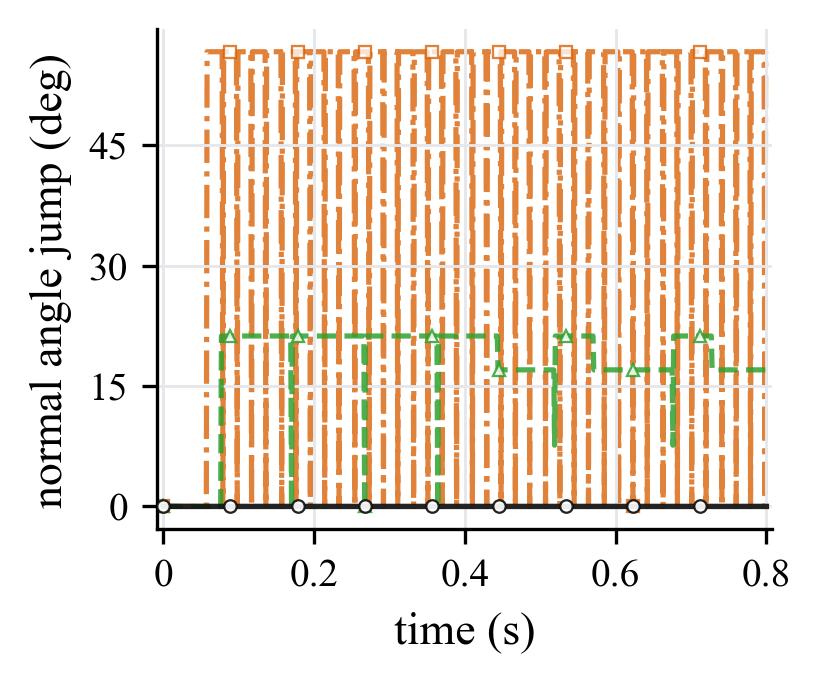
\includegraphics[width=\linewidth]{figures/calg_cmame_used/bearing_ball_raceway_dynamic_backend_curves_normal_angle_jump.png}
\end{minipage}\hfill
\begin{minipage}[t]{0.32\linewidth}
\centering
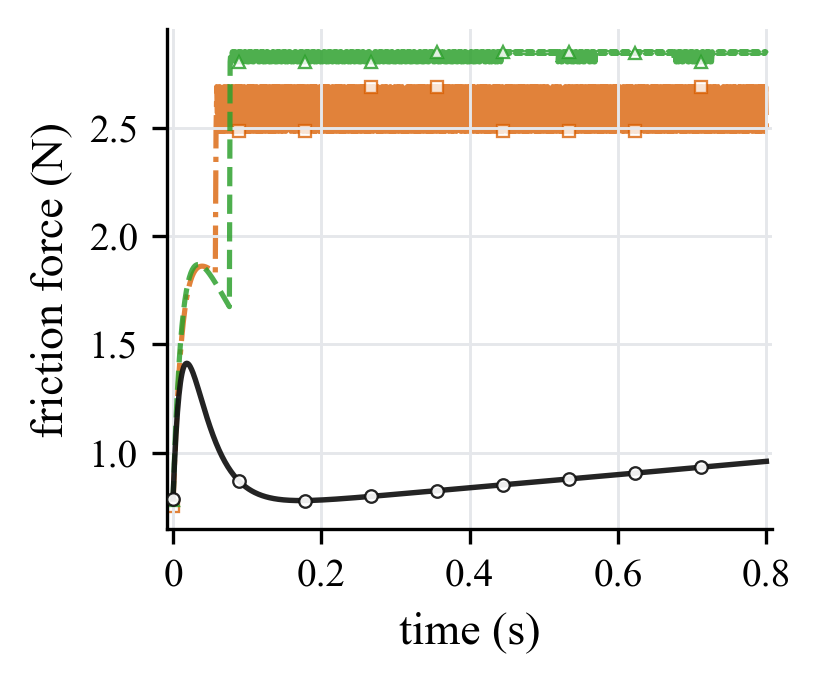
\includegraphics[width=\linewidth]{figures/calg_cmame_used/bearing_ball_raceway_dynamic_backend_curves_friction_force.png}
\end{minipage}\hfill
\begin{minipage}[t]{0.32\linewidth}
\centering
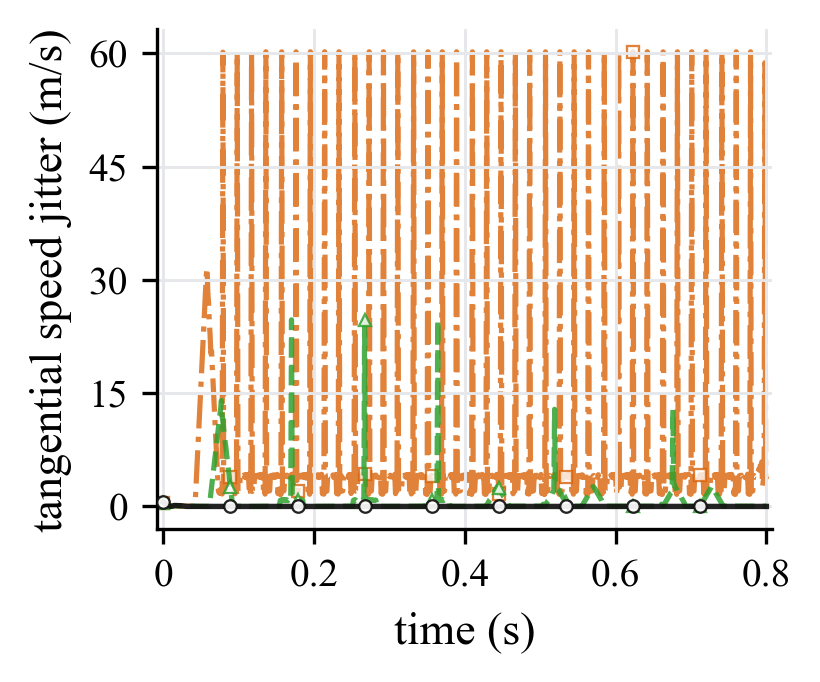
\includegraphics[width=\linewidth]{figures/calg_cmame_used/bearing_ball_raceway_dynamic_backend_curves_tangential_speed_jitter.png}
\end{minipage}
\caption{Independent contact-geometry comparison curves for the Bearing raceway scene. The body state, timestep, penalty stiffness, friction coefficient, and regularized Coulomb update are identical; only the contact-geometry module changes.}
\label{fig:curves_bearing}
\end{figure}

\begin{figure}[t]
\centering
\begin{minipage}[t]{0.32\linewidth}
\centering
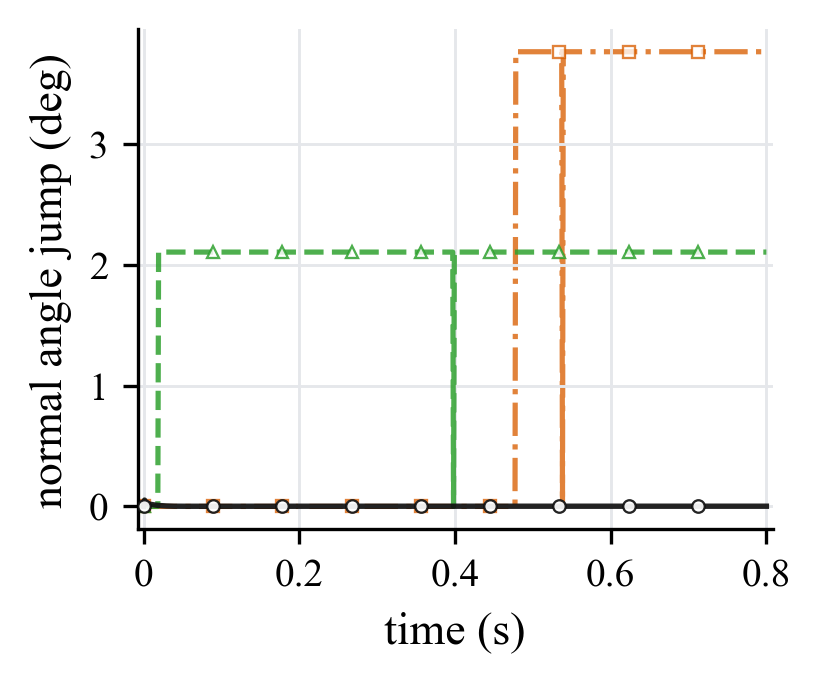
\includegraphics[width=\linewidth]{figures/calg_cmame_used/cam_roller_follower_dynamic_backend_curves_normal_angle_jump.png}
\end{minipage}\hfill
\begin{minipage}[t]{0.32\linewidth}
\centering
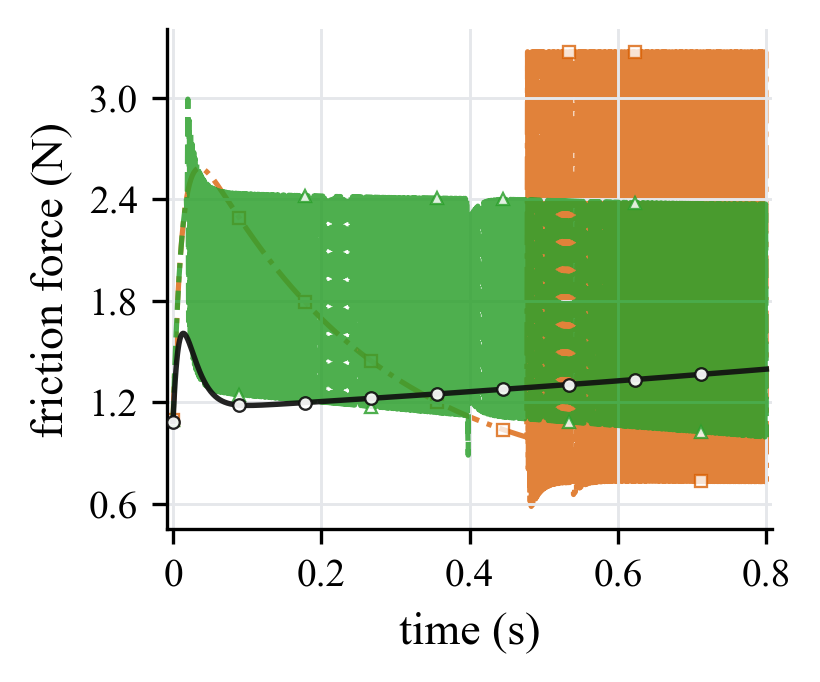
\includegraphics[width=\linewidth]{figures/calg_cmame_used/cam_roller_follower_dynamic_backend_curves_friction_force.png}
\end{minipage}\hfill
\begin{minipage}[t]{0.32\linewidth}
\centering
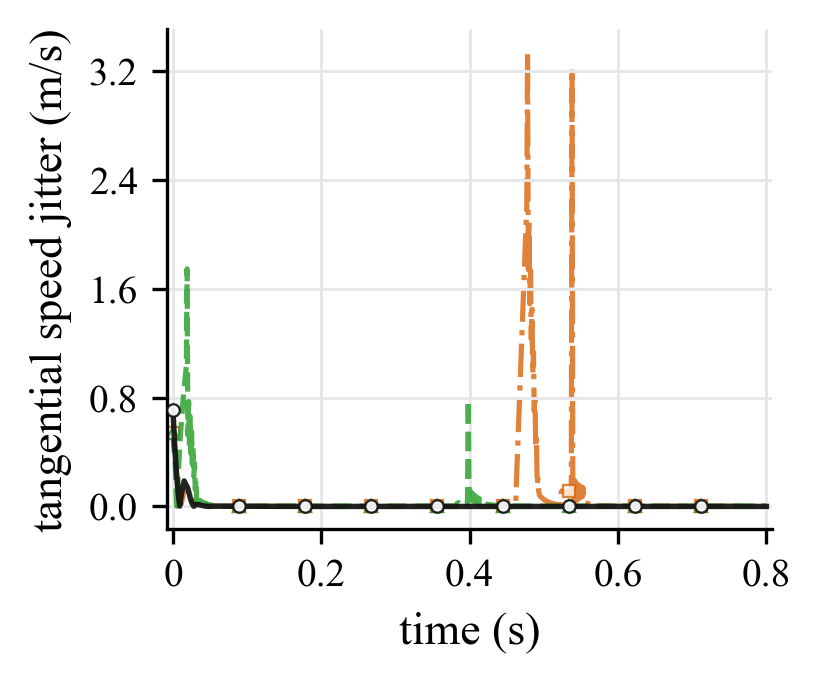
\includegraphics[width=\linewidth]{figures/calg_cmame_used/cam_roller_follower_dynamic_backend_curves_tangential_speed_jitter.png}
\end{minipage}
\caption{Independent contact-geometry comparison curves for the Cam-roller follower scene. Linear-triangle BVH and PN-triangle BVH produce larger normal and friction-force variations when the contact point traverses cam cells.}
\label{fig:curves_cam}
\end{figure}

\begin{figure}[t]
\centering
\begin{minipage}[t]{0.32\linewidth}
\centering
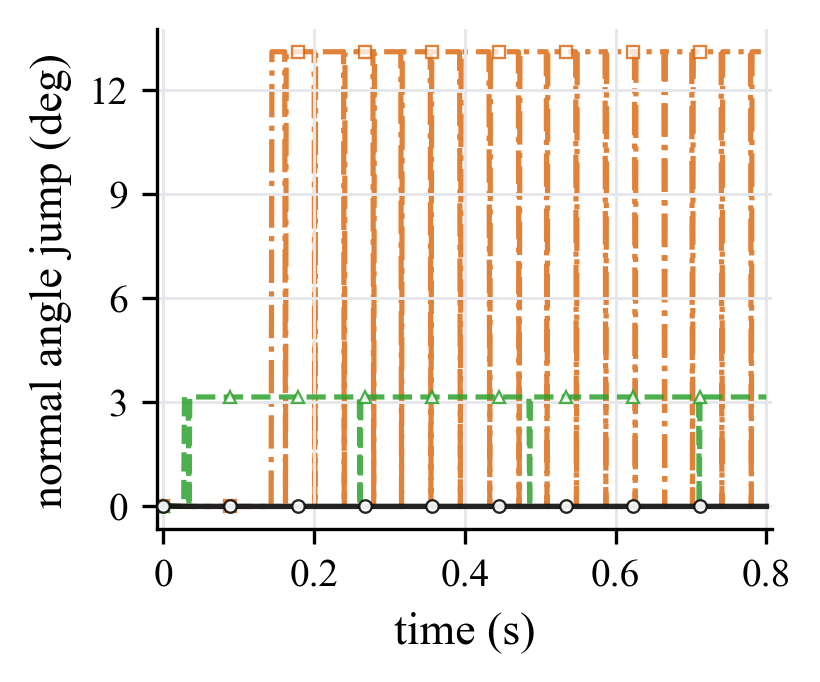
\includegraphics[width=\linewidth]{figures/calg_cmame_used/spherical_joint_socket_dynamic_backend_curves_normal_angle_jump.png}
\end{minipage}\hfill
\begin{minipage}[t]{0.32\linewidth}
\centering
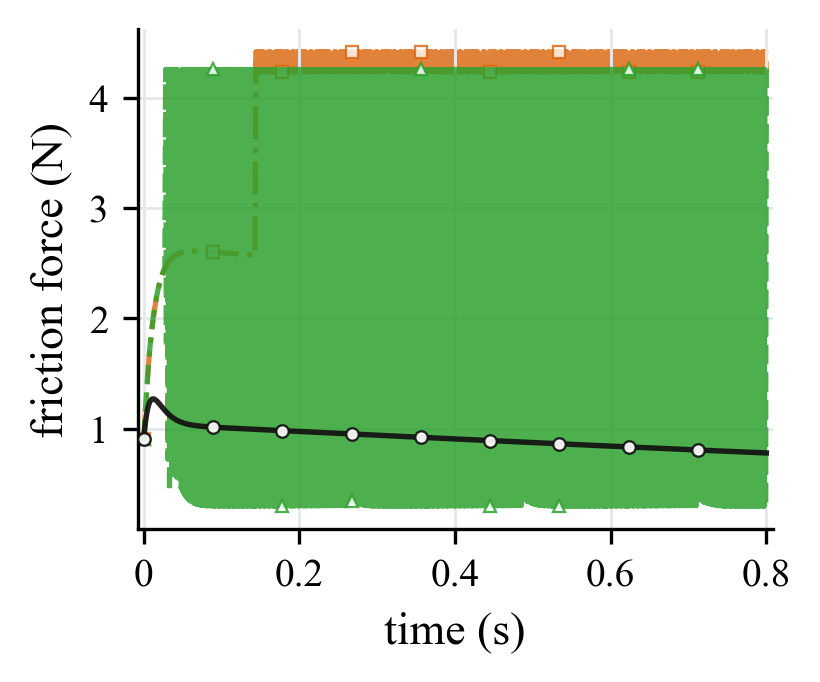
\includegraphics[width=\linewidth]{figures/calg_cmame_used/spherical_joint_socket_dynamic_backend_curves_friction_force.png}
\end{minipage}\hfill
\begin{minipage}[t]{0.32\linewidth}
\centering
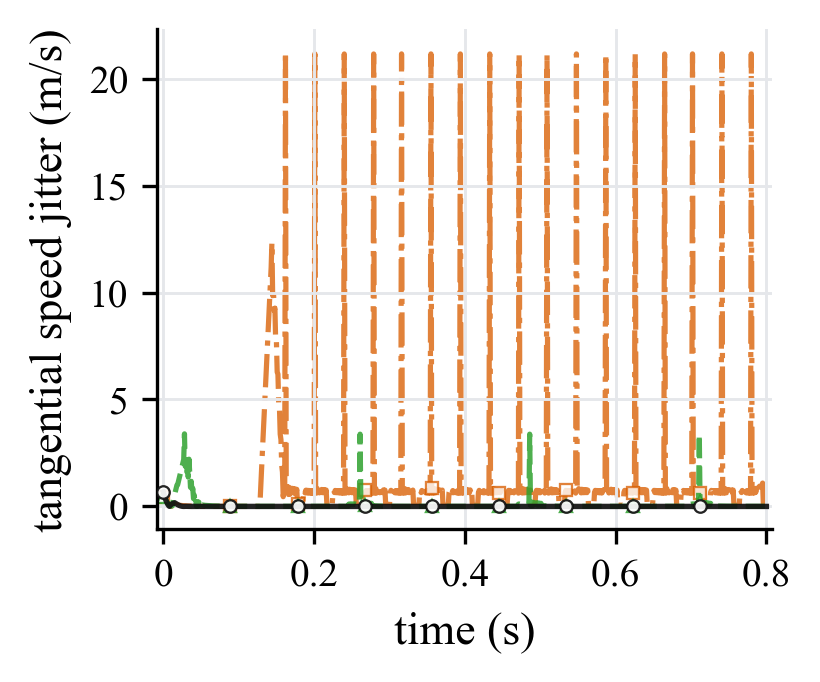
\includegraphics[width=\linewidth]{figures/calg_cmame_used/spherical_joint_socket_dynamic_backend_curves_tangential_speed_jitter.png}
\end{minipage}
\caption{Independent contact-geometry comparison curves for the Ball-and-socket pendulum scene. The smooth \calg{} contact frame suppresses the high-frequency tangential-speed jitter and discrete friction-state changes observed in the fixed-tessellation baselines.}
\label{fig:curves_socket}
\end{figure}

\begin{figure}[t]
\centering
\begin{minipage}[t]{0.32\linewidth}
\centering
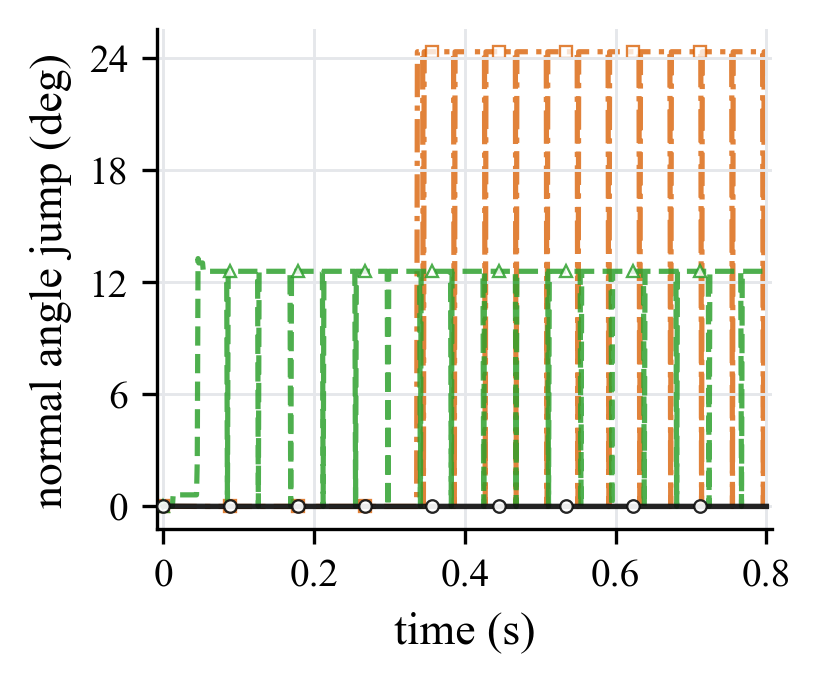
\includegraphics[width=\linewidth]{figures/calg_cmame_used/wavy_guide_slot_ball_head_dynamic_backend_curves_normal_angle_jump.png}
\end{minipage}\hfill
\begin{minipage}[t]{0.32\linewidth}
\centering
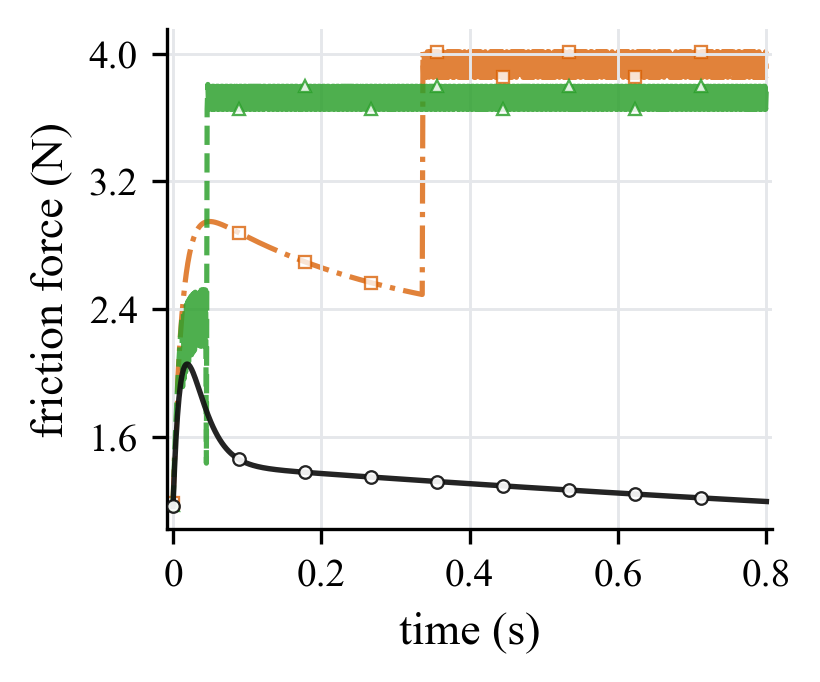
\includegraphics[width=\linewidth]{figures/calg_cmame_used/wavy_guide_slot_ball_head_dynamic_backend_curves_friction_force.png}
\end{minipage}\hfill
\begin{minipage}[t]{0.32\linewidth}
\centering
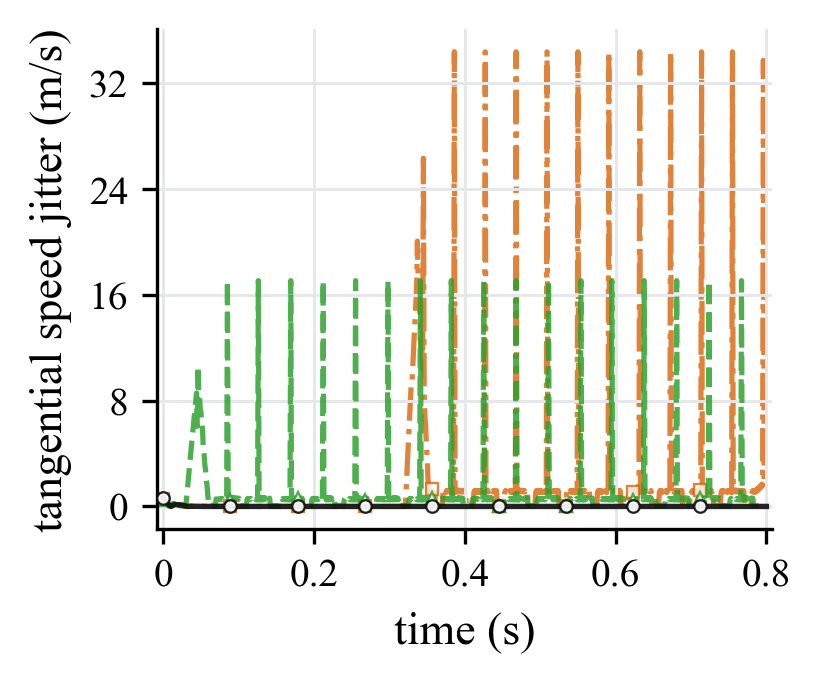
\includegraphics[width=\linewidth]{figures/calg_cmame_used/wavy_guide_slot_ball_head_dynamic_backend_curves_tangential_speed_jitter.png}
\end{minipage}
\caption{Independent contact-geometry comparison curves for the Guide slot scene. Cell-crossing normal changes in the Linear-triangle BVH and PN-triangle BVH modules enter directly into friction-force and tangential-speed jitter.}
\label{fig:curves_guide}
\end{figure}

\FloatBarrier

The dynamic results support the central mechanism of the method. Linear-triangle BVH consistently generates much larger geometric and force discontinuities: the normal-angle jump ratio ranges from $71.9$ to $2.20\times10^3$, the normal-force jump ratio from $44.2$ to $1.50\times10^3$, the friction-force jump ratio from $37.7$ to $108$, and the tangential-speed jitter ratio from $23.8$ to $2.20\times10^3$. PN-triangle BVH improves over Linear-triangle BVH in several scenes, but it remains tied to a tessellated approximation and still produces $40.2$--$826$ times larger normal-angle jumps and $35.8$--$62.6$ times larger friction-force jumps than \calg{}. The large stick--slip switch ratios for Linear-triangle BVH in the Cam-roller follower scene and for PN-triangle BVH in the Ball-and-socket pendulum scene show that smoother geometry affects not only the gap value but also the discrete friction state.

\subsection{External validation against Chrono and Recurdyn}

The matched contact-geometry comparison isolates the geometric input to the friction response, but it does not by itself show that the resulting motion is consistent with independent dynamics engines. We therefore reproduced three selected engineering scenes in Chrono, Recurdyn, and the \calg{} detector-driven rigid contact model: Guide slot, Ball-and-socket pendulum, and Bearing raceway. Each scene uses the same model description, rigid-body mass and geometry, initial state, friction coefficient, and timestep where applicable. In the \calg{} C++ runs, the local curved mesh detector supplies candidate/contact work and a configuration-space SDF refines the signed gap and normal over a small surface-contact response patch; the regularized normal and friction responses are assembled by the normalized quadrature in Eq.~\eqref{eq:response_quadrature}. Chrono and Recurdyn use different contact envelopes and regularizations, so the validation target is trajectory-level agreement in displacement and velocity trends rather than pointwise equality of raw contact force.

In all trajectory-validation figures, the black solid curve denotes \calg{}, the blue dashed curve denotes Chrono, and the orange dash-dot curve denotes Recurdyn; sparse open markers are used only to separate nearly overlapping traces. The plotted directions are the three Cartesian ball coordinates, and displacements are relative to each solver's initial ball coordinate.

The Guide slot scene tests confined sliding under wall contact, so the expected response is sustained sliding along the slot while the side wall confines transverse motion. The \calg{} C++ run uses a sphere of radius $0.090$ m and mass $0.75$ kg, initial positive gap $2.0\times10^{-3}$ m, initial speed $0.58$ m/s along the guide, $T=3.0$ s, 6000 steps, $\Delta t=5.0\times10^{-4}$ s, $\mu=0.40$, detector band $0.018$ m, $k_n/c_n=8.0\times10^4/520$, release tolerance $5.0\times10^{-4}$ m, response patch radius $0.0035$ m, and $Q=4$ normalized response samples. Figures~\ref{fig:guide_slot_displacement}-\ref{fig:guide_slot_acceleration} show that the three solvers produce the same sliding direction, comparable transverse confinement, and bounded acceleration after visualization smoothing. This visual agreement in the dominant displacement and velocity trends is the intended validation target for the Guide slot scene. The limitation is that acceleration is a diagnostic channel rather than a strict pointwise validation target: \calg{}, Chrono, and Recurdyn export or reconstruct acceleration through different contact-force and envelope definitions.

\begin{figure}[t]
\centering
\begin{minipage}{0.32\linewidth}
\centering
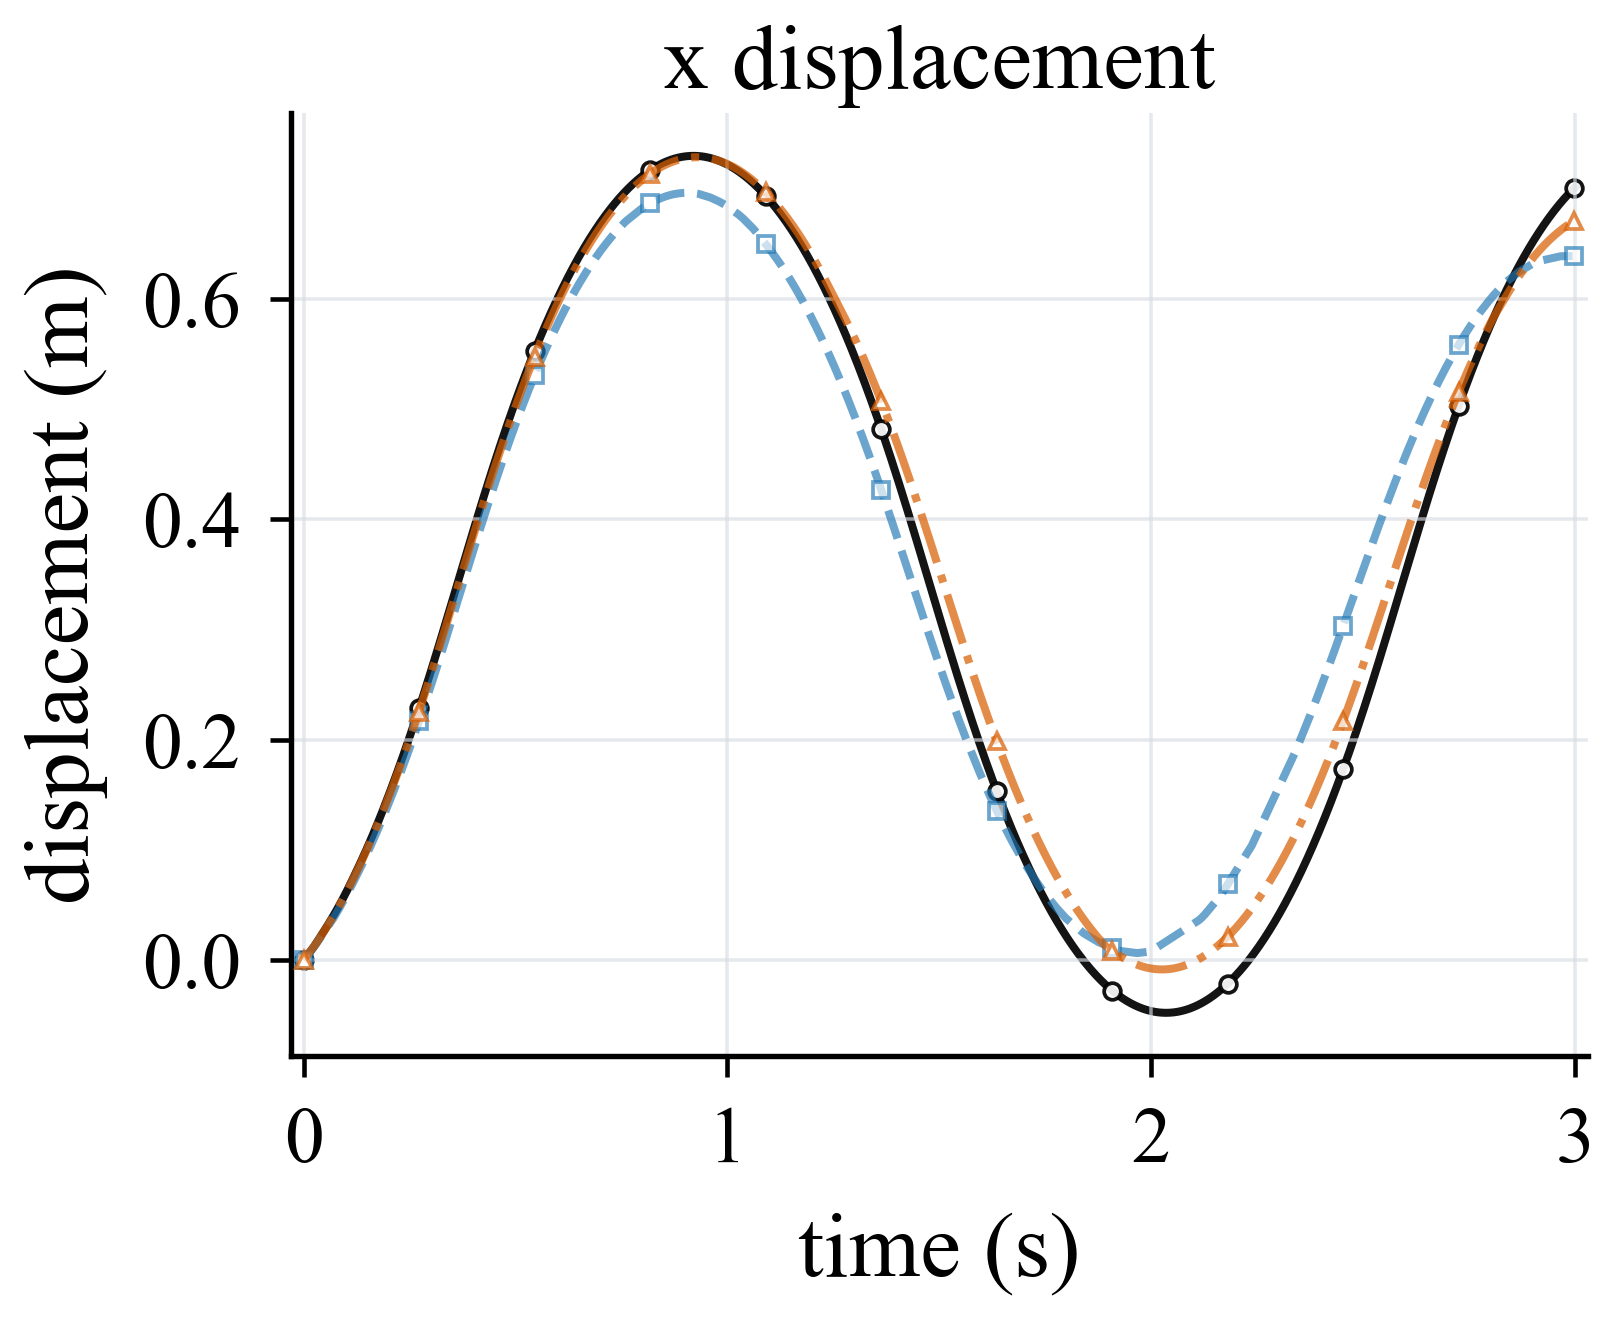
\includegraphics[width=\linewidth]{figures/calg_cmame_used/03_guide_slot_3s_x_displacement.png}
\end{minipage}\hfill
\begin{minipage}{0.32\linewidth}
\centering
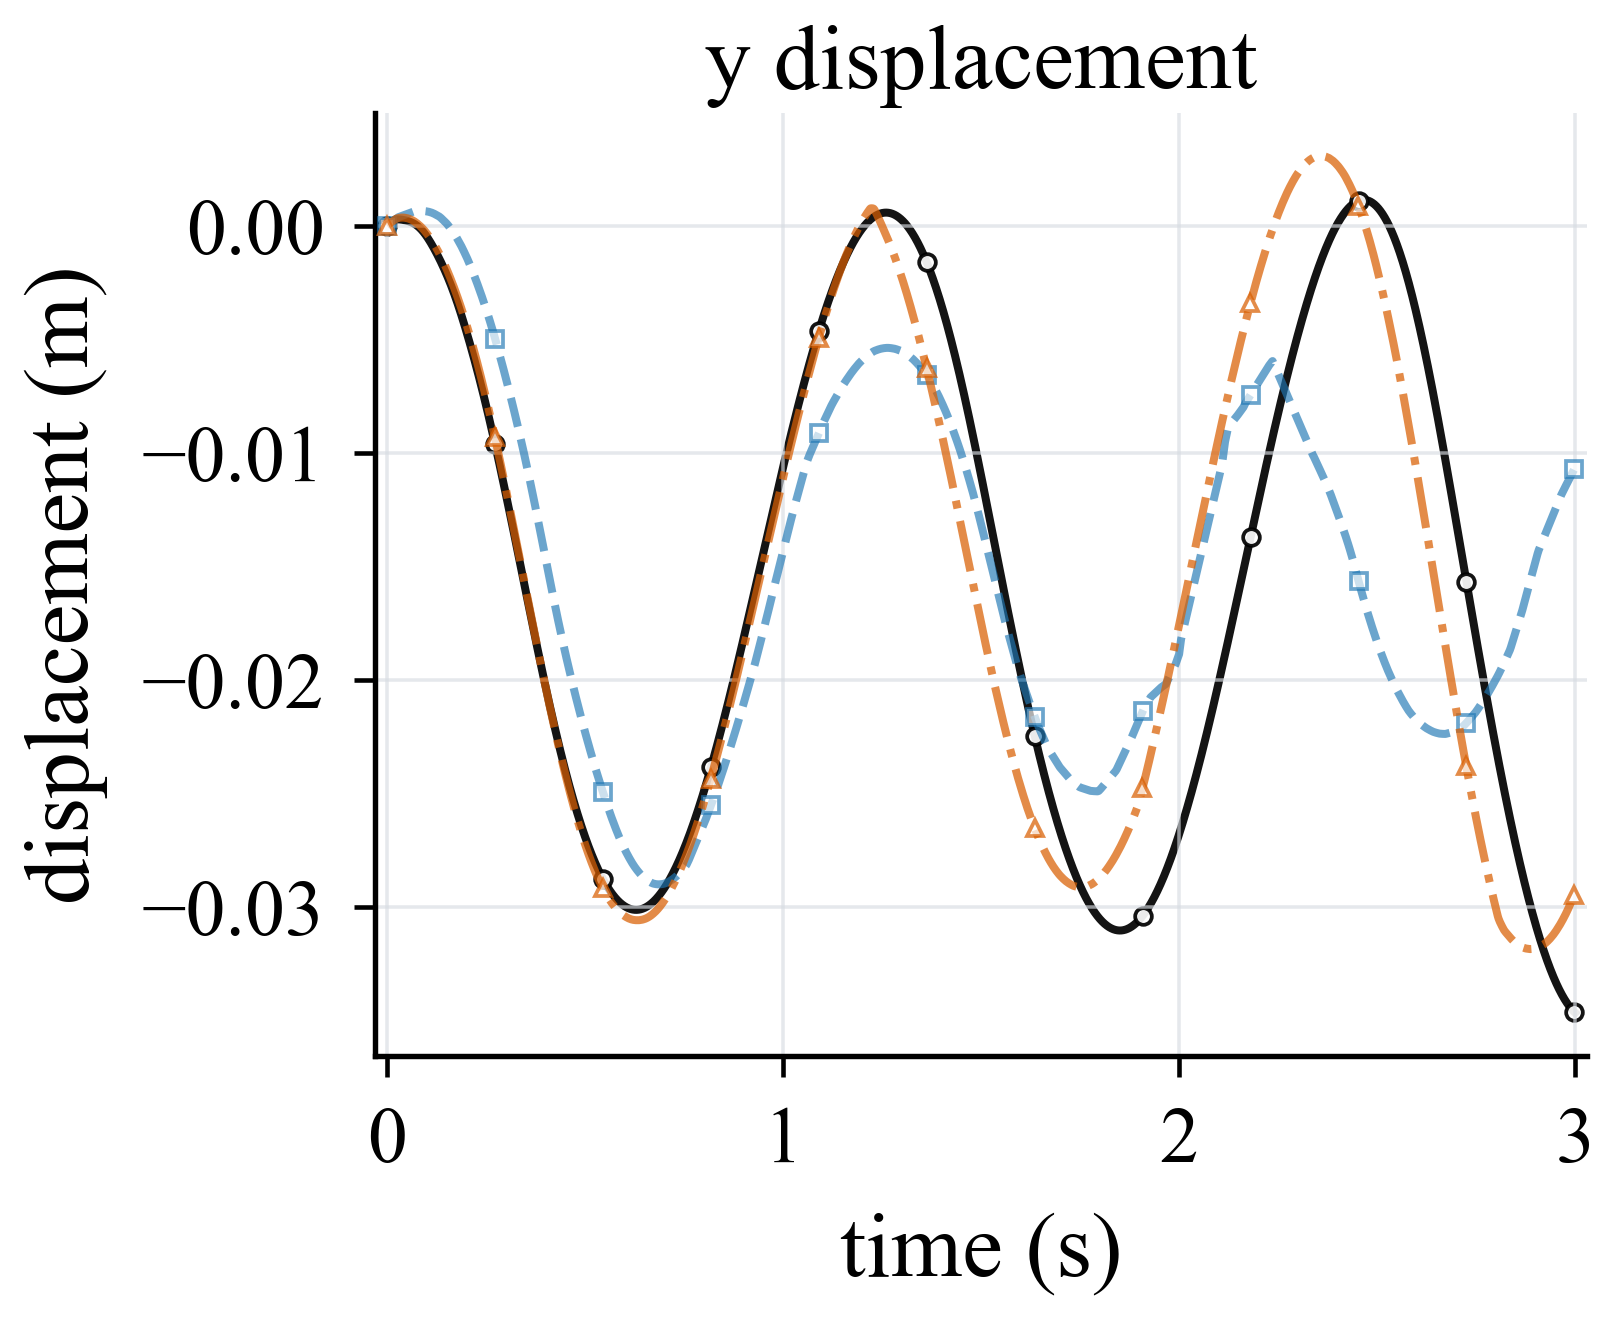
\includegraphics[width=\linewidth]{figures/calg_cmame_used/03_guide_slot_3s_y_displacement.png}
\end{minipage}\hfill
\begin{minipage}{0.32\linewidth}
\centering
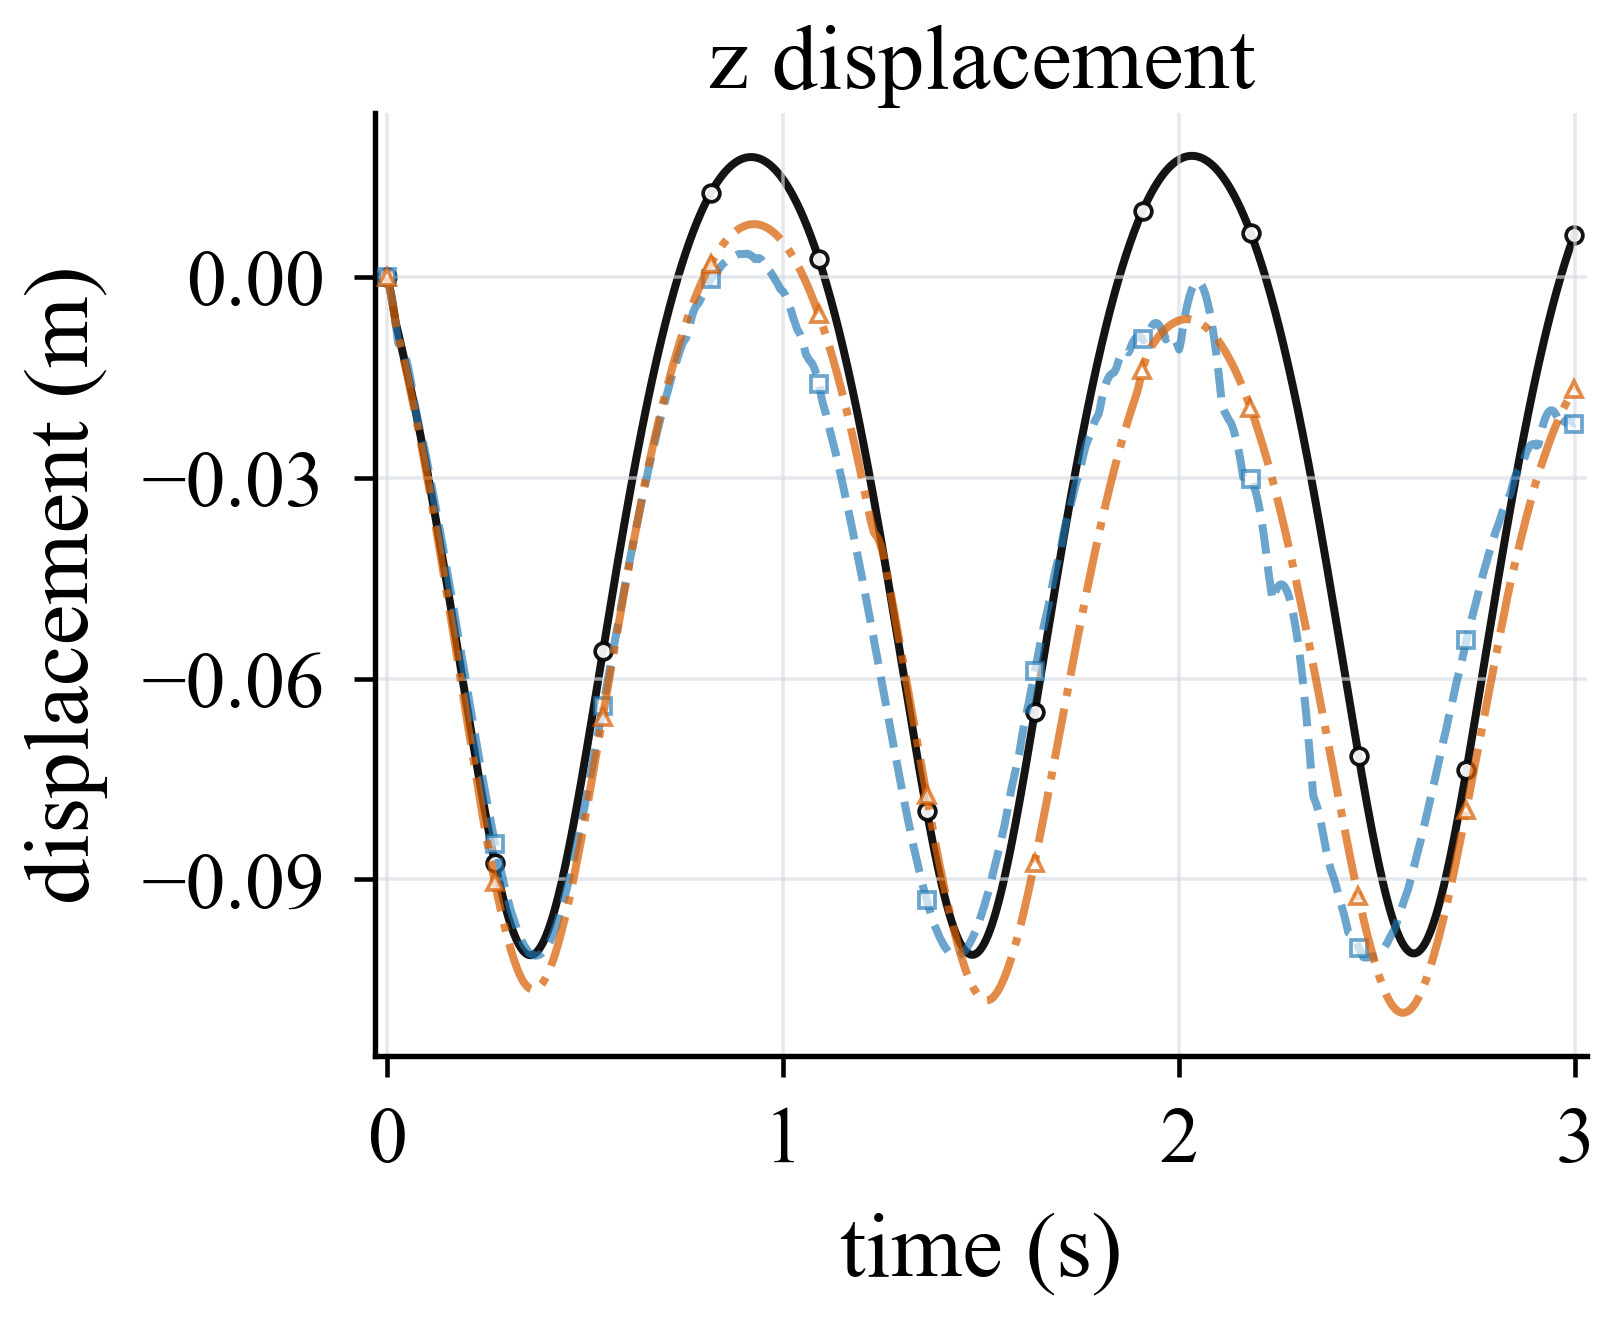
\includegraphics[width=\linewidth]{figures/calg_cmame_used/03_guide_slot_3s_z_displacement.png}
\end{minipage}
\caption{Guide slot validation over 3 s: ball displacement in the $x$, $y$, and $z$ directions. The \calg{} result is shown as the black solid curve; displacements are relative to each solver's initial ball coordinate.}
\label{fig:guide_slot_displacement}
\end{figure}

\begin{figure}[t]
\centering
\begin{minipage}{0.32\linewidth}
\centering
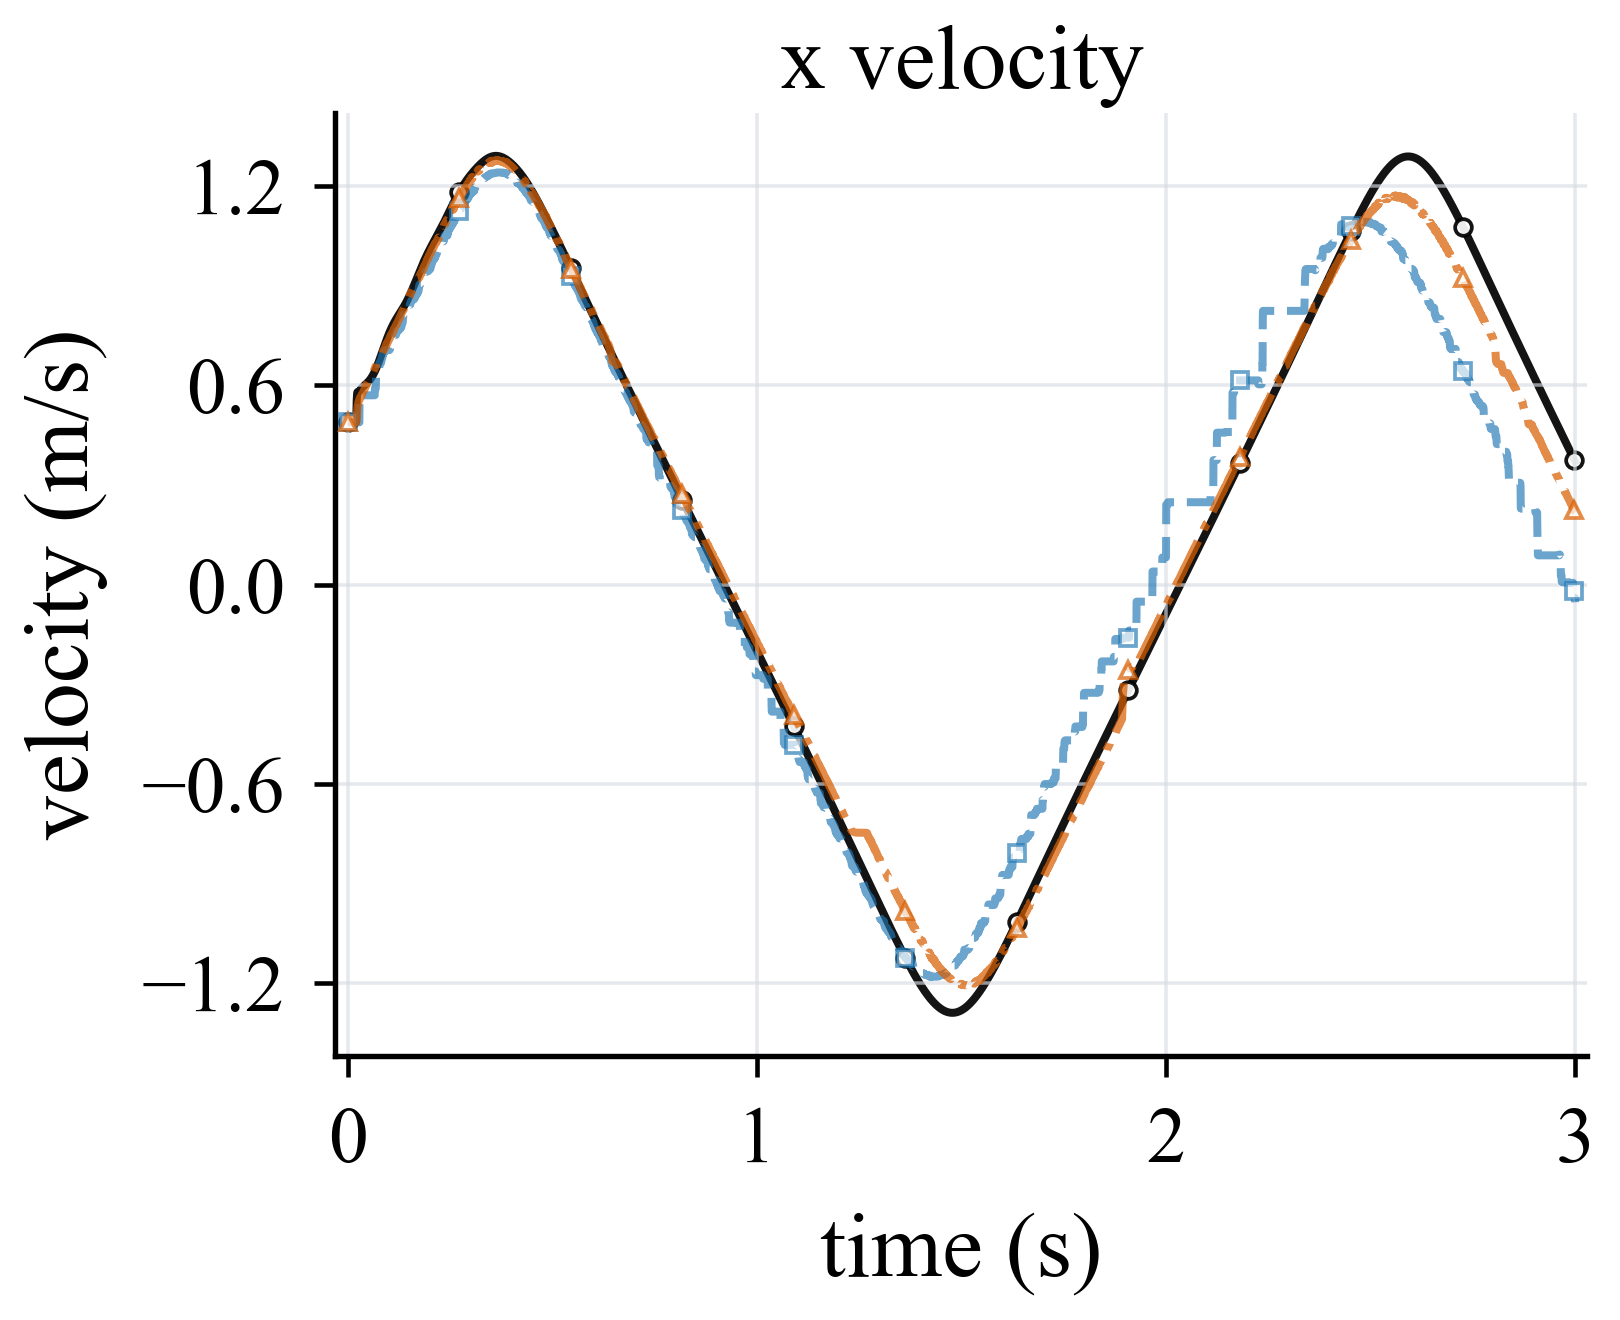
\includegraphics[width=\linewidth]{figures/calg_cmame_used/03_guide_slot_3s_x_velocity.png}
\end{minipage}\hfill
\begin{minipage}{0.32\linewidth}
\centering
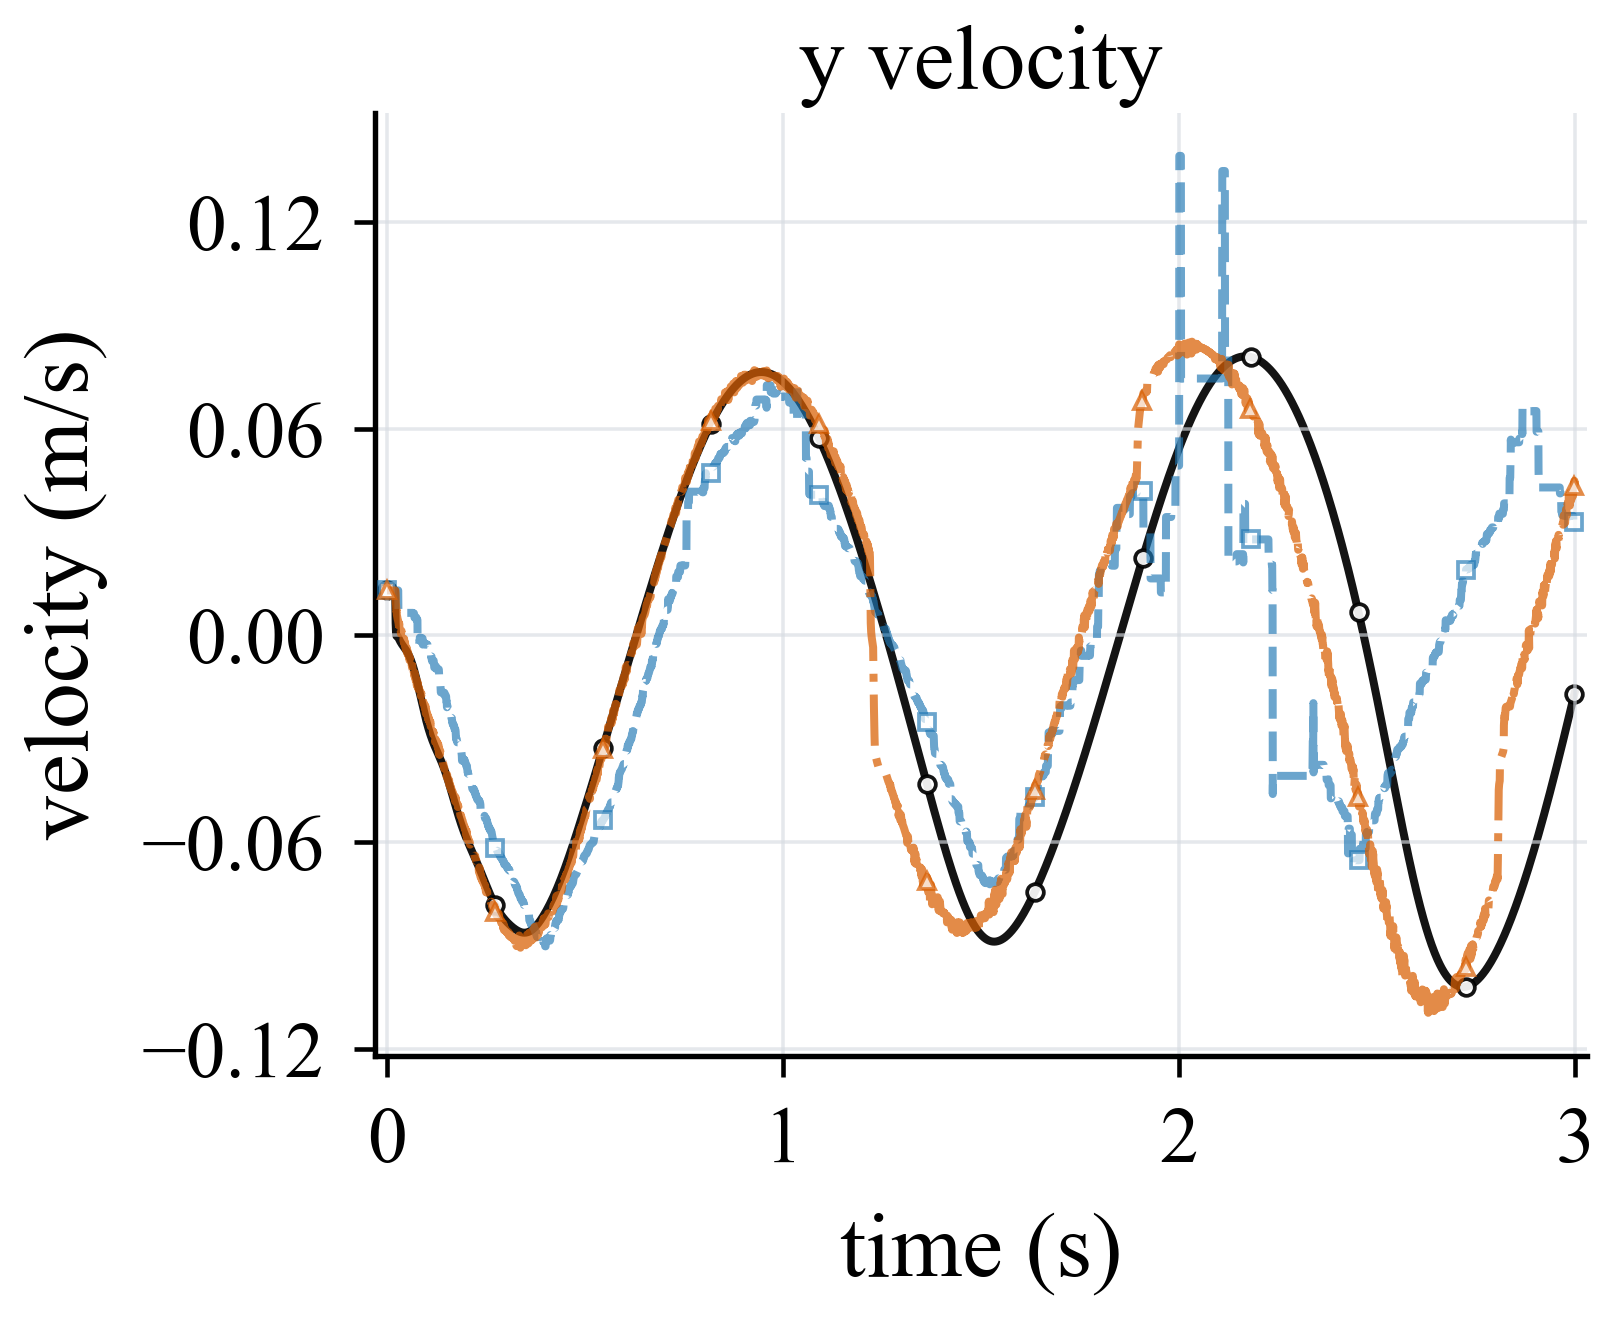
\includegraphics[width=\linewidth]{figures/calg_cmame_used/03_guide_slot_3s_y_velocity.png}
\end{minipage}\hfill
\begin{minipage}{0.32\linewidth}
\centering
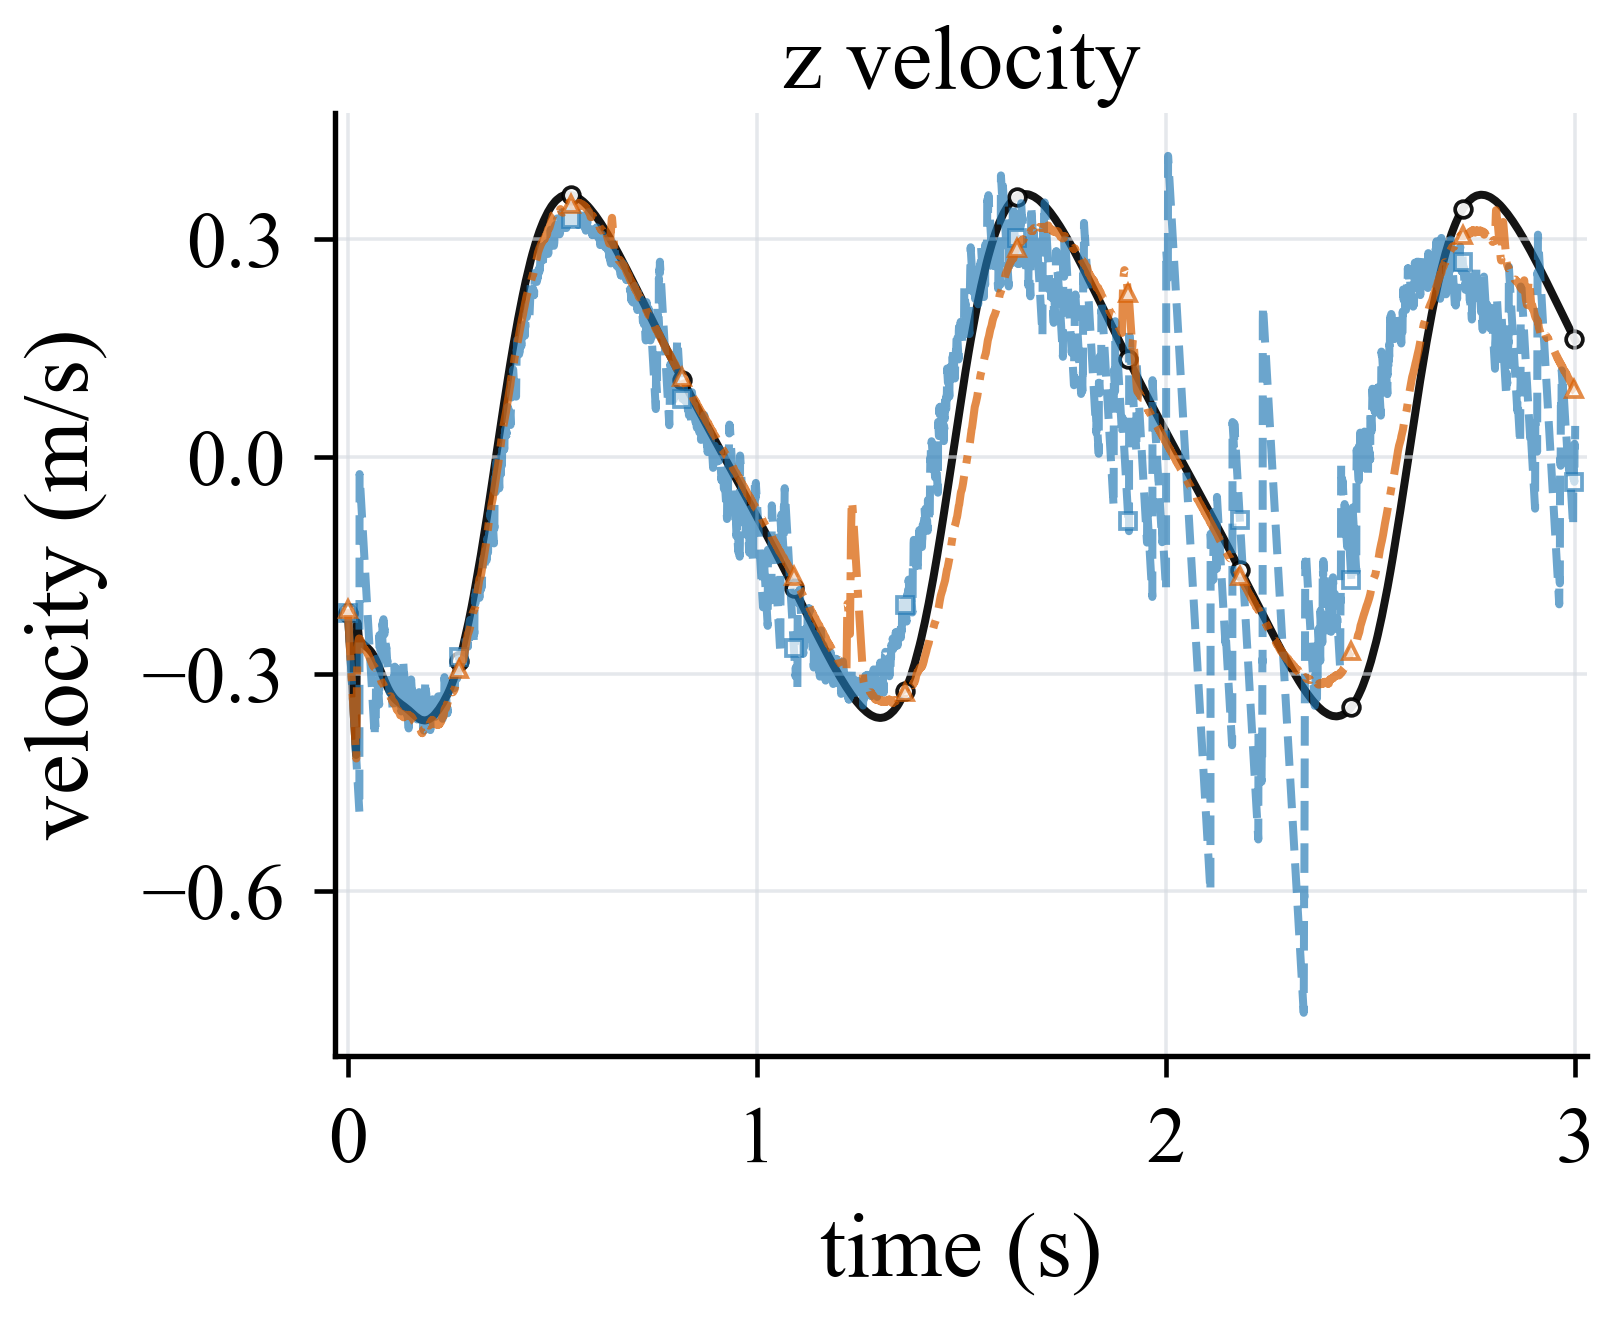
\includegraphics[width=\linewidth]{figures/calg_cmame_used/03_guide_slot_3s_z_velocity.png}
\end{minipage}
\caption{Guide slot validation over 3 s: ball velocity in the $x$, $y$, and $z$ directions. The \calg{} result is shown as the black solid curve.}
\label{fig:guide_slot_velocity}
\end{figure}

\begin{figure}[t]
\centering
\begin{minipage}{0.32\linewidth}
\centering
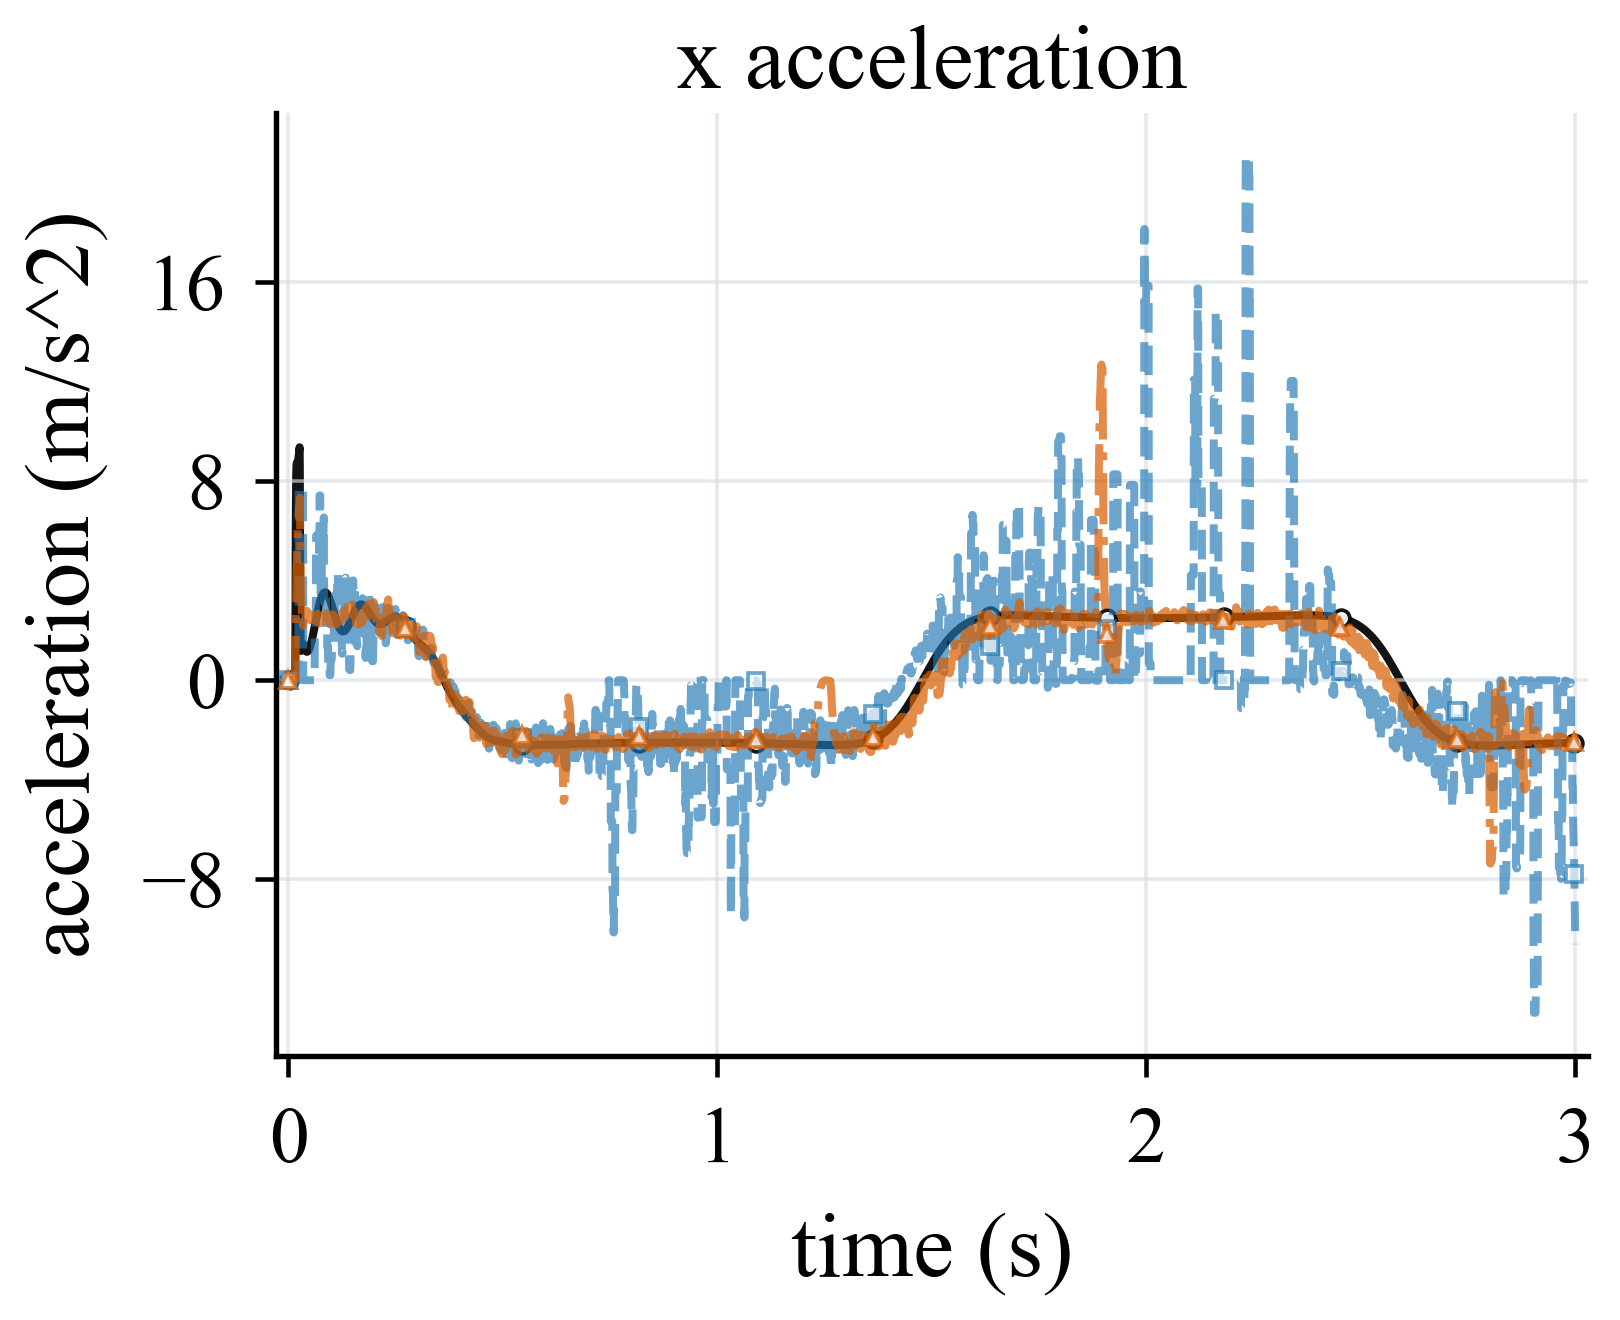
\includegraphics[width=\linewidth]{figures/calg_cmame_used/03_guide_slot_3s_x_acceleration.png}
\end{minipage}\hfill
\begin{minipage}{0.32\linewidth}
\centering
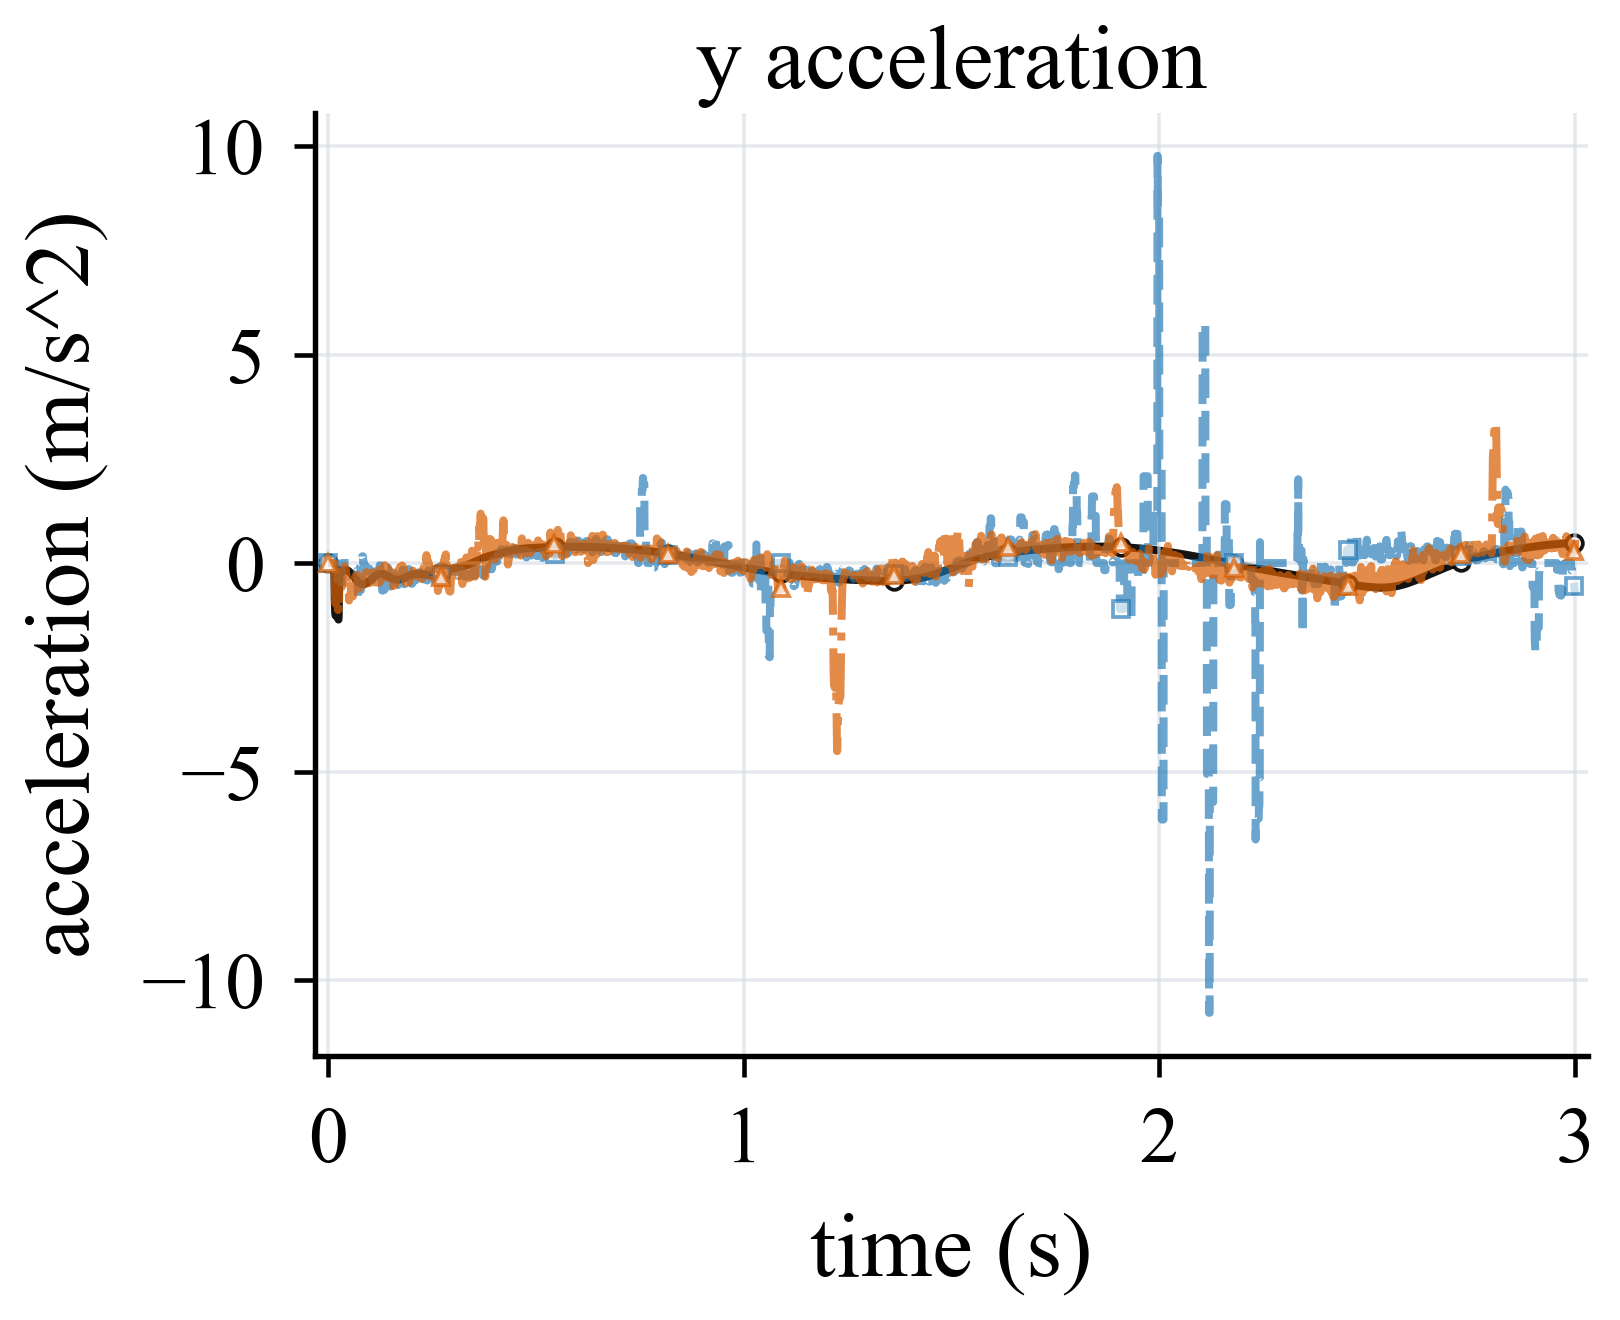
\includegraphics[width=\linewidth]{figures/calg_cmame_used/03_guide_slot_3s_y_acceleration.png}
\end{minipage}\hfill
\begin{minipage}{0.32\linewidth}
\centering
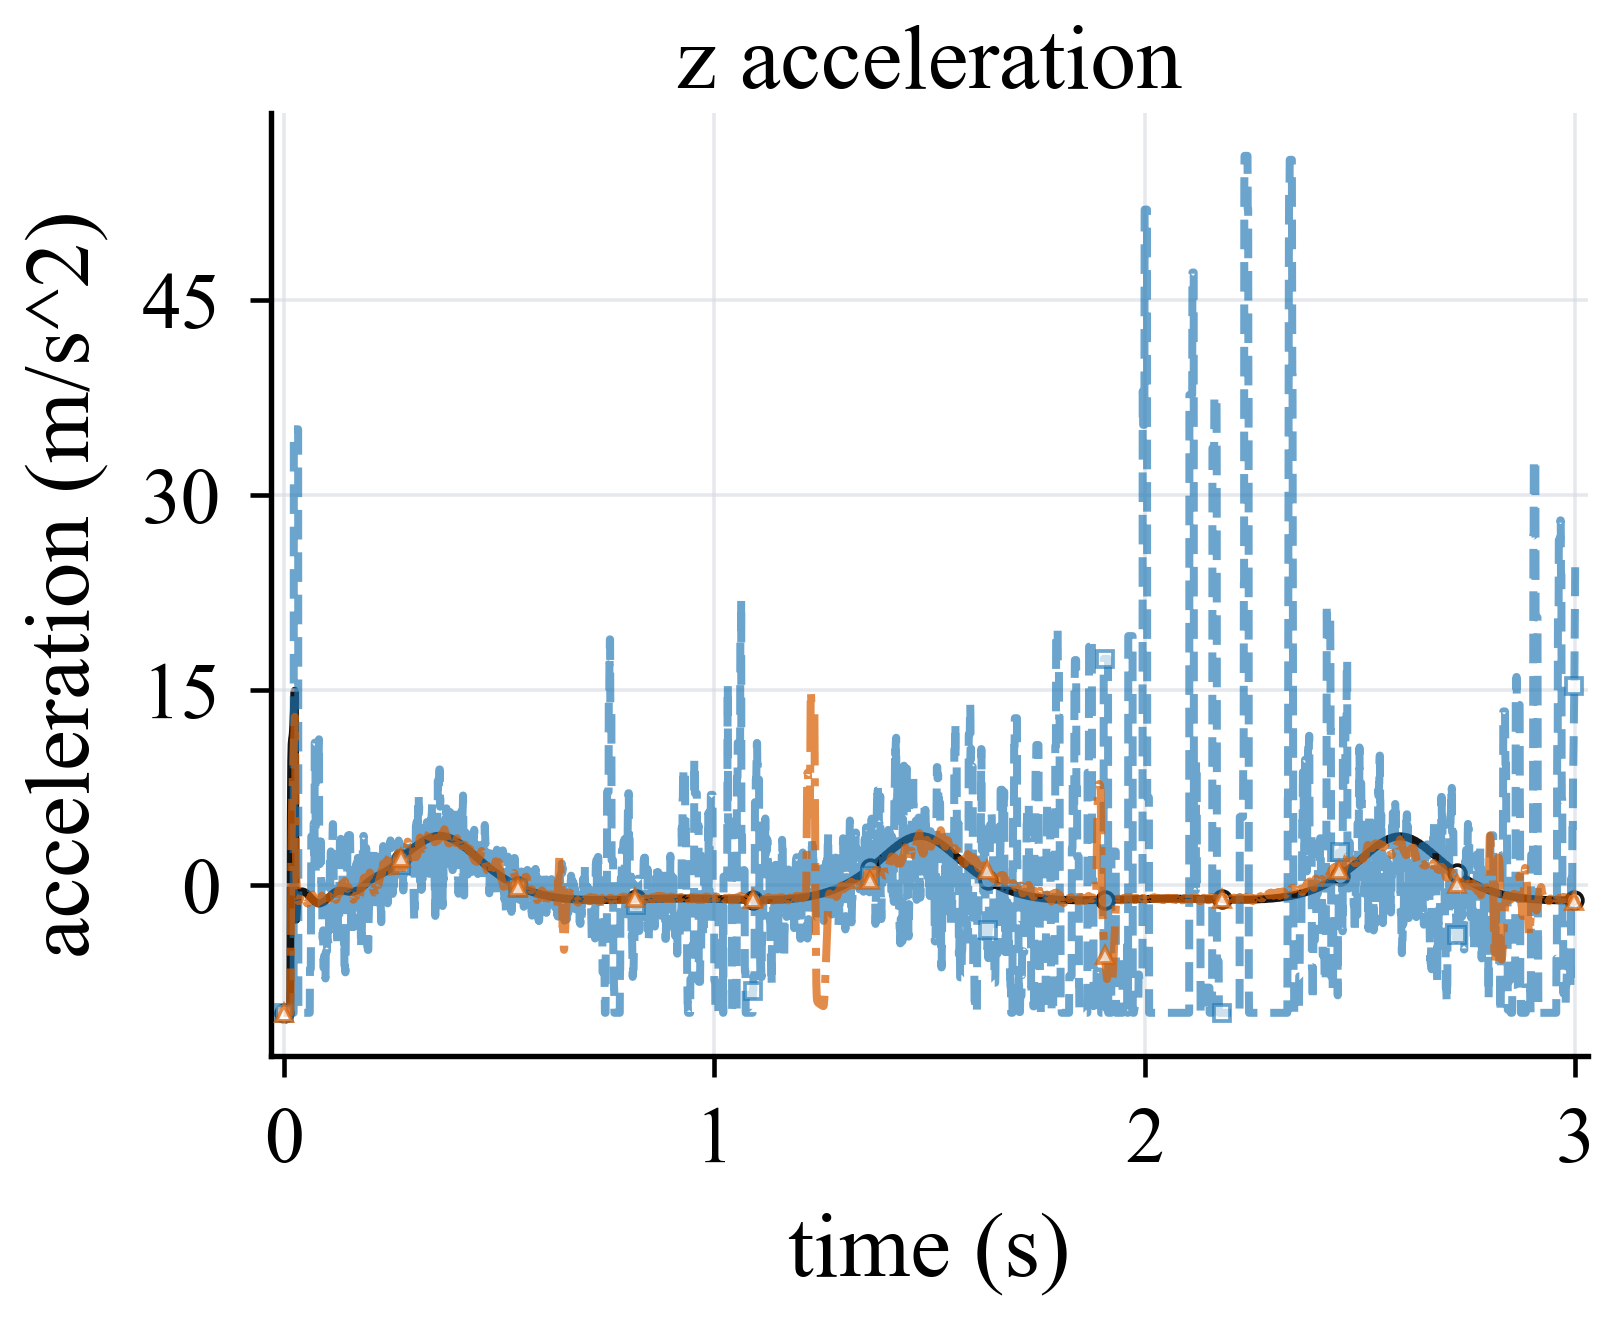
\includegraphics[width=\linewidth]{figures/calg_cmame_used/03_guide_slot_3s_z_acceleration.png}
\end{minipage}
\caption{Guide slot validation over 3 s: ball acceleration in the $x$, $y$, and $z$ directions. For \calg{}, acceleration is the effective per-step value exported by the C++ implementation after the normal-constraint and gap-clamp update; for Chrono it is evaluated from the reported contact force and gravity; for Recurdyn it is taken from the exported body-acceleration channels. The plotted curves use a 21-frame centered average for visualization.}
\label{fig:guide_slot_acceleration}
\end{figure}
\FloatBarrier

The Ball-and-socket pendulum scene tests gravity-driven swing under deep socket confinement, so the expected response is pendular motion with socket-limited contact. The model uses a socket with inner radius $0.42$ m, outer radius $0.50$ m, and opening polar angle $0.42$ rad; the moving assembly contains a ball of radius $0.34$ m, a rod of radius $0.035$ m and length $0.82$ m, and a distal payload of radius $0.115$ m. The \calg{} C++ run uses $T=5.0$ s, 25000 steps, $\Delta t=2.0\times10^{-4}$ s, $\mu=0.35$, detector band $0.012$ m, $k_n/c_n=2.0\times10^5/650$, release tolerance $1.2\times10^{-3}$ m, response patch radius $0.0040$ m, and $Q=4$ normalized response samples. Figures~\ref{fig:ball_joint_displacement}-\ref{fig:ball_joint_acceleration} compare the same 5 s window after matching the Recurdyn moving-body mass distribution to the rod-plus-cylinder assembly used by Chrono and \calg{}. The first vertical pendulum peak occurs at $1.1438$ s in Chrono, $1.1304$ s in \calg{}, and $1.1252$ s in Recurdyn, with peak vertical displacements of $0.1255$, $0.1330$, and $0.1383$ m, respectively. These comparable peak timings and amplitudes support the physical reasonableness of the \calg{} trajectory. The remaining discrepancy is concentrated in re-contact transients and raw acceleration, where the three solvers use different contact regularizations and contact-envelope definitions.

\begin{figure}[t]
\centering
\begin{minipage}{0.32\linewidth}
\centering
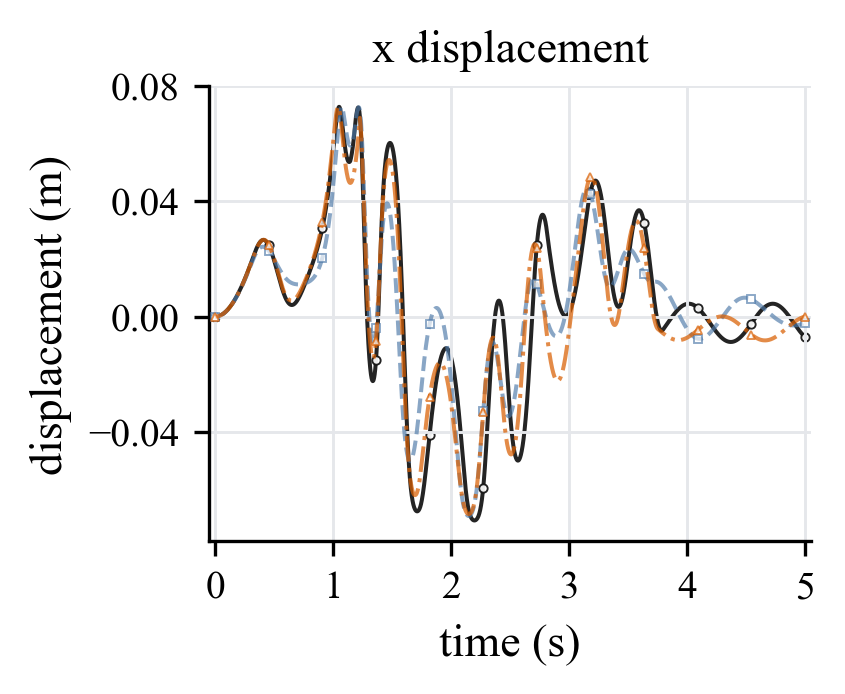
\includegraphics[width=\linewidth]{figures/calg_cmame_used/03_ball_joint_5s_equiv_payload_x_displacement.png}
\end{minipage}\hfill
\begin{minipage}{0.32\linewidth}
\centering
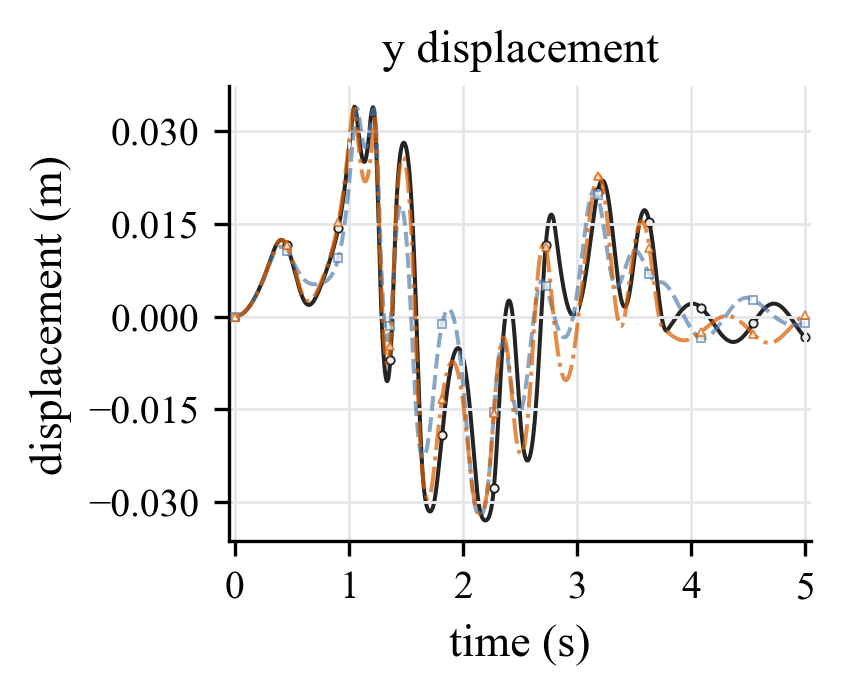
\includegraphics[width=\linewidth]{figures/calg_cmame_used/03_ball_joint_5s_equiv_payload_y_displacement.png}
\end{minipage}\hfill
\begin{minipage}{0.32\linewidth}
\centering
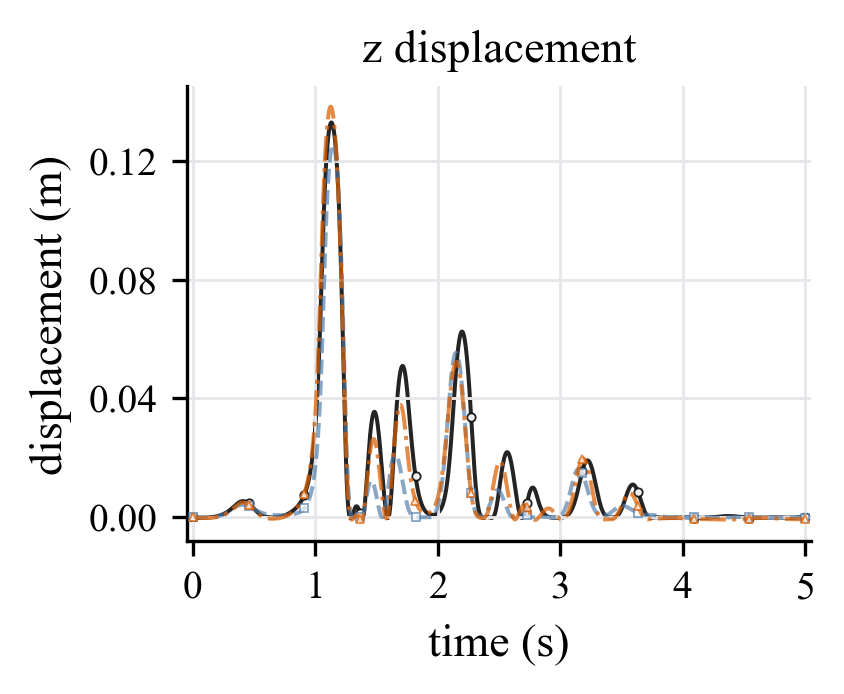
\includegraphics[width=\linewidth]{figures/calg_cmame_used/03_ball_joint_5s_equiv_payload_z_displacement.png}
\end{minipage}
\caption{Ball-and-socket pendulum validation over 5 s: ball displacement in the $x$, $y$, and $z$ directions. The Recurdyn model uses an equivalent distal payload with the same rod-plus-cylinder mass center and inertia as the Chrono and \calg{} composite body. The \calg{} result is shown as the black solid curve; displacements are relative to each solver's initial ball coordinate.}
\label{fig:ball_joint_displacement}
\end{figure}

\begin{figure}[t]
\centering
\begin{minipage}{0.32\linewidth}
\centering
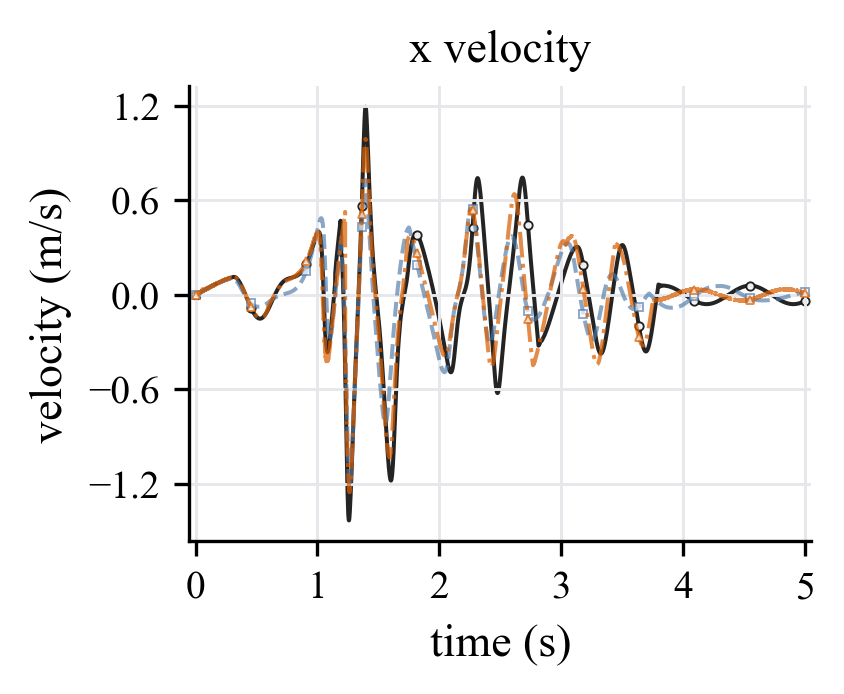
\includegraphics[width=\linewidth]{figures/calg_cmame_used/03_ball_joint_5s_equiv_payload_x_velocity.png}
\end{minipage}\hfill
\begin{minipage}{0.32\linewidth}
\centering
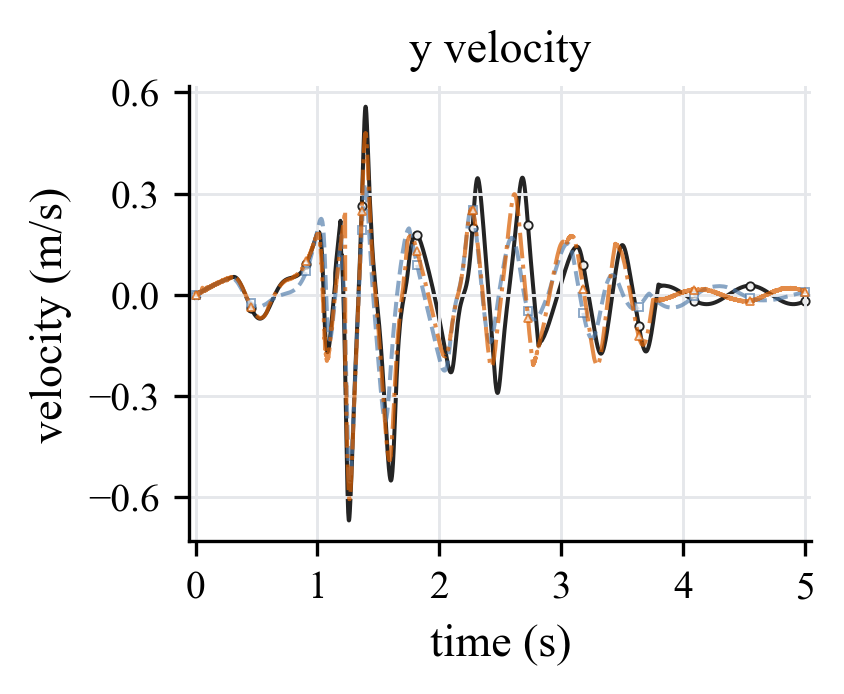
\includegraphics[width=\linewidth]{figures/calg_cmame_used/03_ball_joint_5s_equiv_payload_y_velocity.png}
\end{minipage}\hfill
\begin{minipage}{0.32\linewidth}
\centering
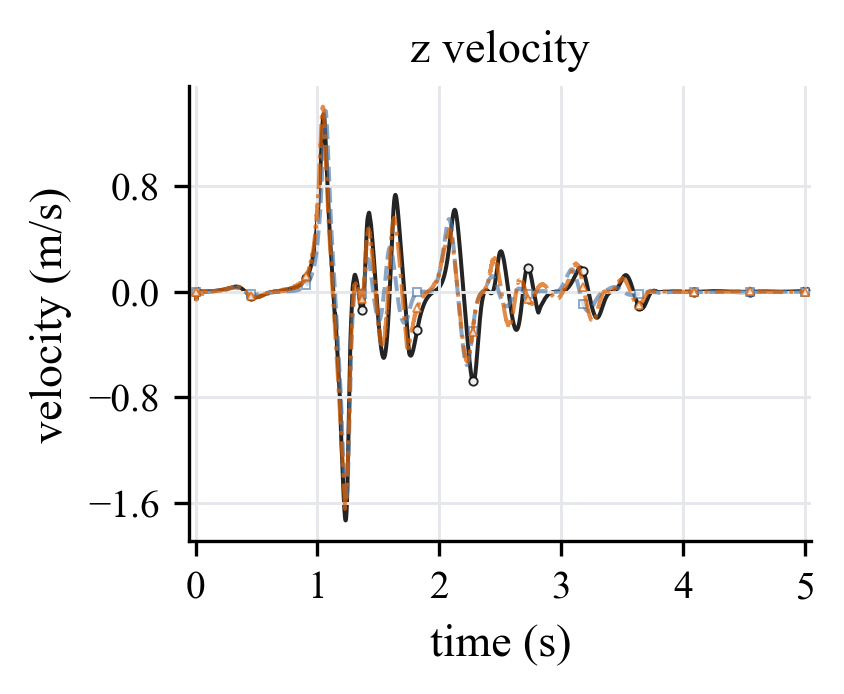
\includegraphics[width=\linewidth]{figures/calg_cmame_used/03_ball_joint_5s_equiv_payload_z_velocity.png}
\end{minipage}
\caption{Ball-and-socket pendulum validation over 5 s: ball velocity in the $x$, $y$, and $z$ directions. The dominant motion trend is consistent across Chrono, Recurdyn, and \calg{}, while re-contact transients remain solver dependent.}
\label{fig:ball_joint_velocity}
\end{figure}

\begin{figure}[t]
\centering
\begin{minipage}{0.32\linewidth}
\centering
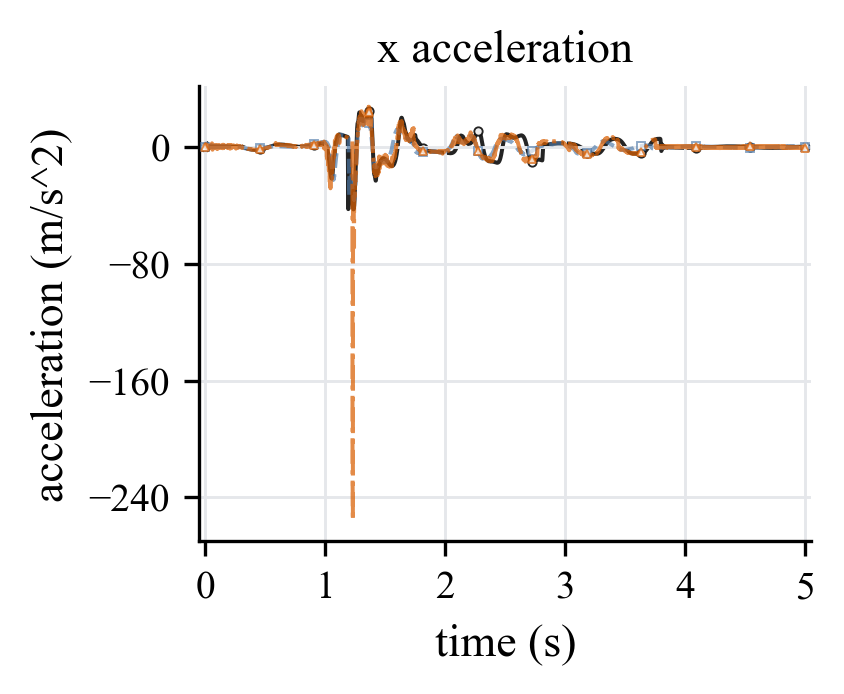
\includegraphics[width=\linewidth]{figures/calg_cmame_used/03_ball_joint_5s_equiv_payload_x_acceleration.png}
\end{minipage}\hfill
\begin{minipage}{0.32\linewidth}
\centering
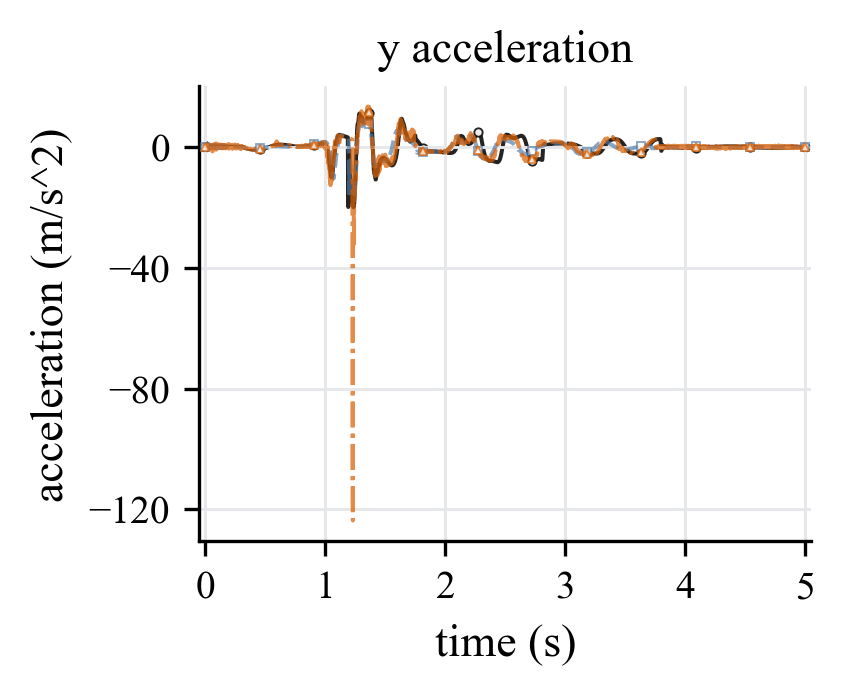
\includegraphics[width=\linewidth]{figures/calg_cmame_used/03_ball_joint_5s_equiv_payload_y_acceleration.png}
\end{minipage}\hfill
\begin{minipage}{0.32\linewidth}
\centering
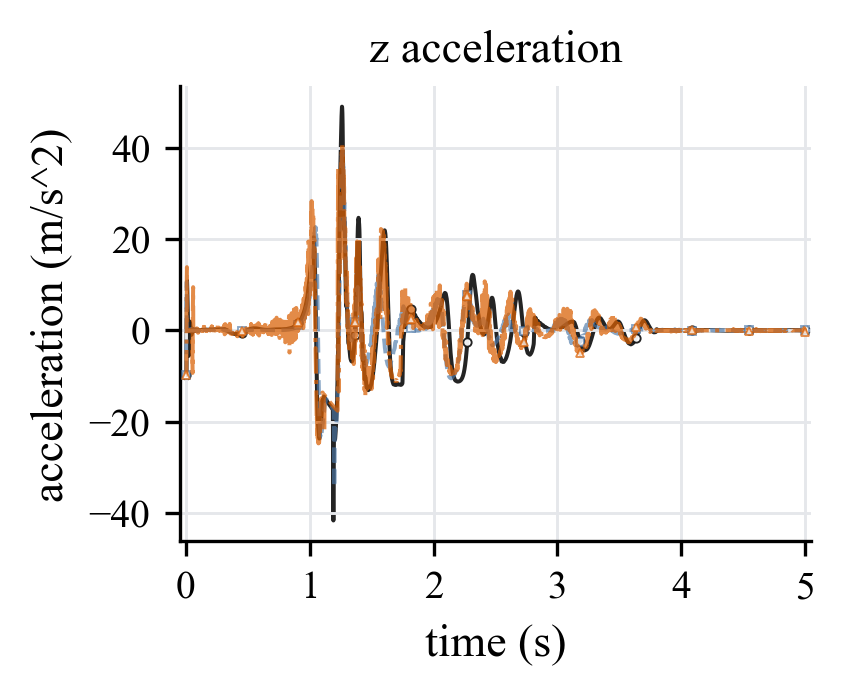
\includegraphics[width=\linewidth]{figures/calg_cmame_used/03_ball_joint_5s_equiv_payload_z_acceleration.png}
\end{minipage}
\caption{Ball-and-socket pendulum validation over 5 s: ball acceleration in the $x$, $y$, and $z$ directions. Accelerations are shown as diagnostic channels for the contact transient; the displacement and velocity curves provide the primary trajectory-level validation because the three solvers use different contact regularizations and contact-envelope definitions.}
\label{fig:ball_joint_acceleration}
\end{figure}
\FloatBarrier

The Bearing raceway scene tests raceway-driven in-plane rolling/sliding, with the axial $z$ direction retained as a small diagnostic channel. The model uses track radius $1.0$ m, groove radius $0.161$ m, preload $2.0\times10^{-4}$ m, ball radius $0.1612$ m, inner-ring angular speed $0.036$ rad/s, and initial ball speed $0.015$ m/s. The \calg{} C++ run uses $T=5.0$ s, 10000 steps, $\Delta t=5.0\times10^{-4}$ s, $\mu=0.08$, detector band $0.010$ m, $k_n/c_n=700/28$, response patch radius $0.0040$ m, $Q=4$ normalized response samples, and a dense SDF grid of $181\times181\times81$. Figures~\ref{fig:bearing_displacement}-\ref{fig:bearing_acceleration} show that the dominant $x$ and $y$ displacement and velocity curves follow the imposed raceway motion over 5 s in all three solvers. The small axial response is retained to expose contact-envelope differences rather than to define the main motion. The Recurdyn contact stiffness is raised to $1.0\times10^8$ with damping $1.5\times10^4$ to reduce vertical over-penetration, but raw contact force and post-processed gap remain envelope-dependent and are not used as strict pointwise validation targets.

\begin{figure}[t]
\centering
\begin{minipage}{0.32\linewidth}
\centering

\includegraphics[width=\linewidth]{figures/calg_cmame_used/03_bearing_5s_x_displacement.png}
\end{minipage}\hfill
\begin{minipage}{0.32\linewidth}
\centering
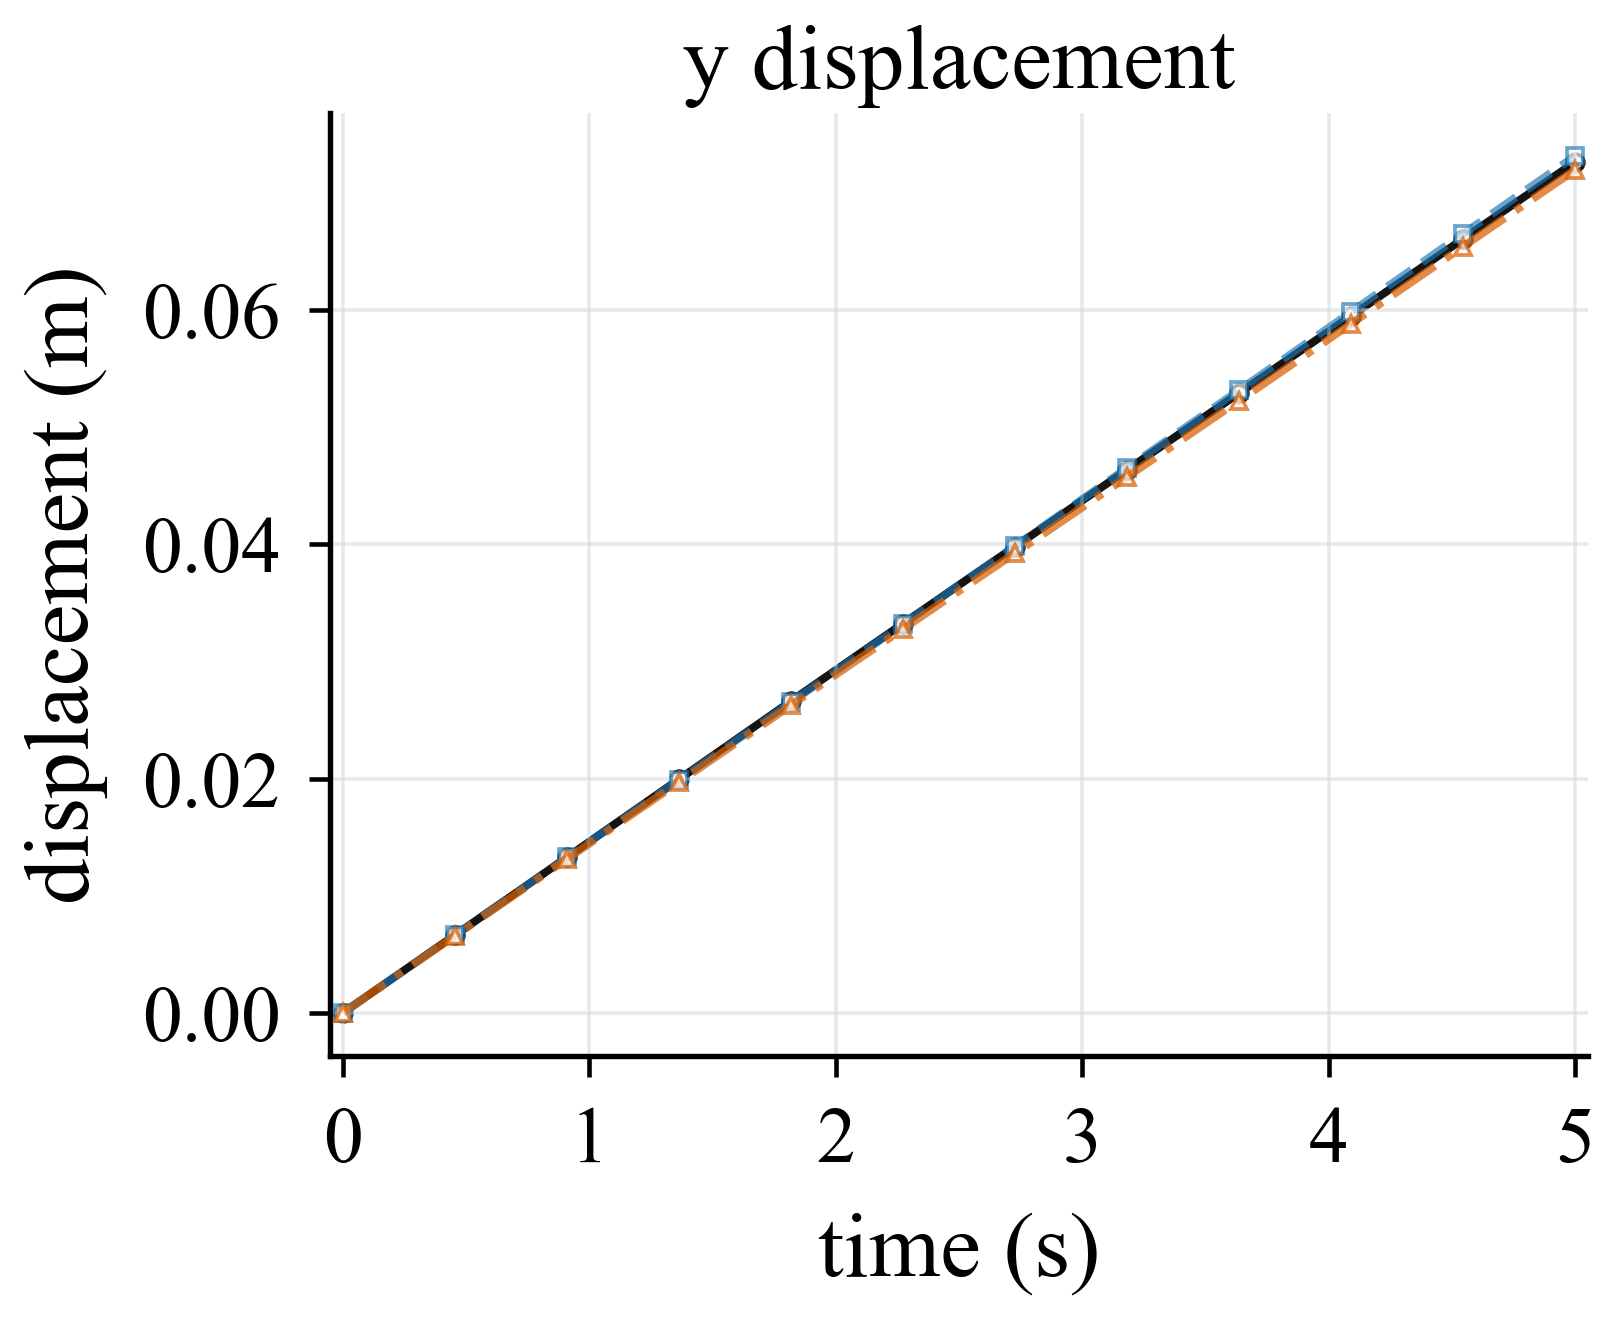
\includegraphics[width=\linewidth]{figures/calg_cmame_used/03_bearing_5s_y_displacement.png}
\end{minipage}\hfill
\begin{minipage}{0.32\linewidth}
\centering
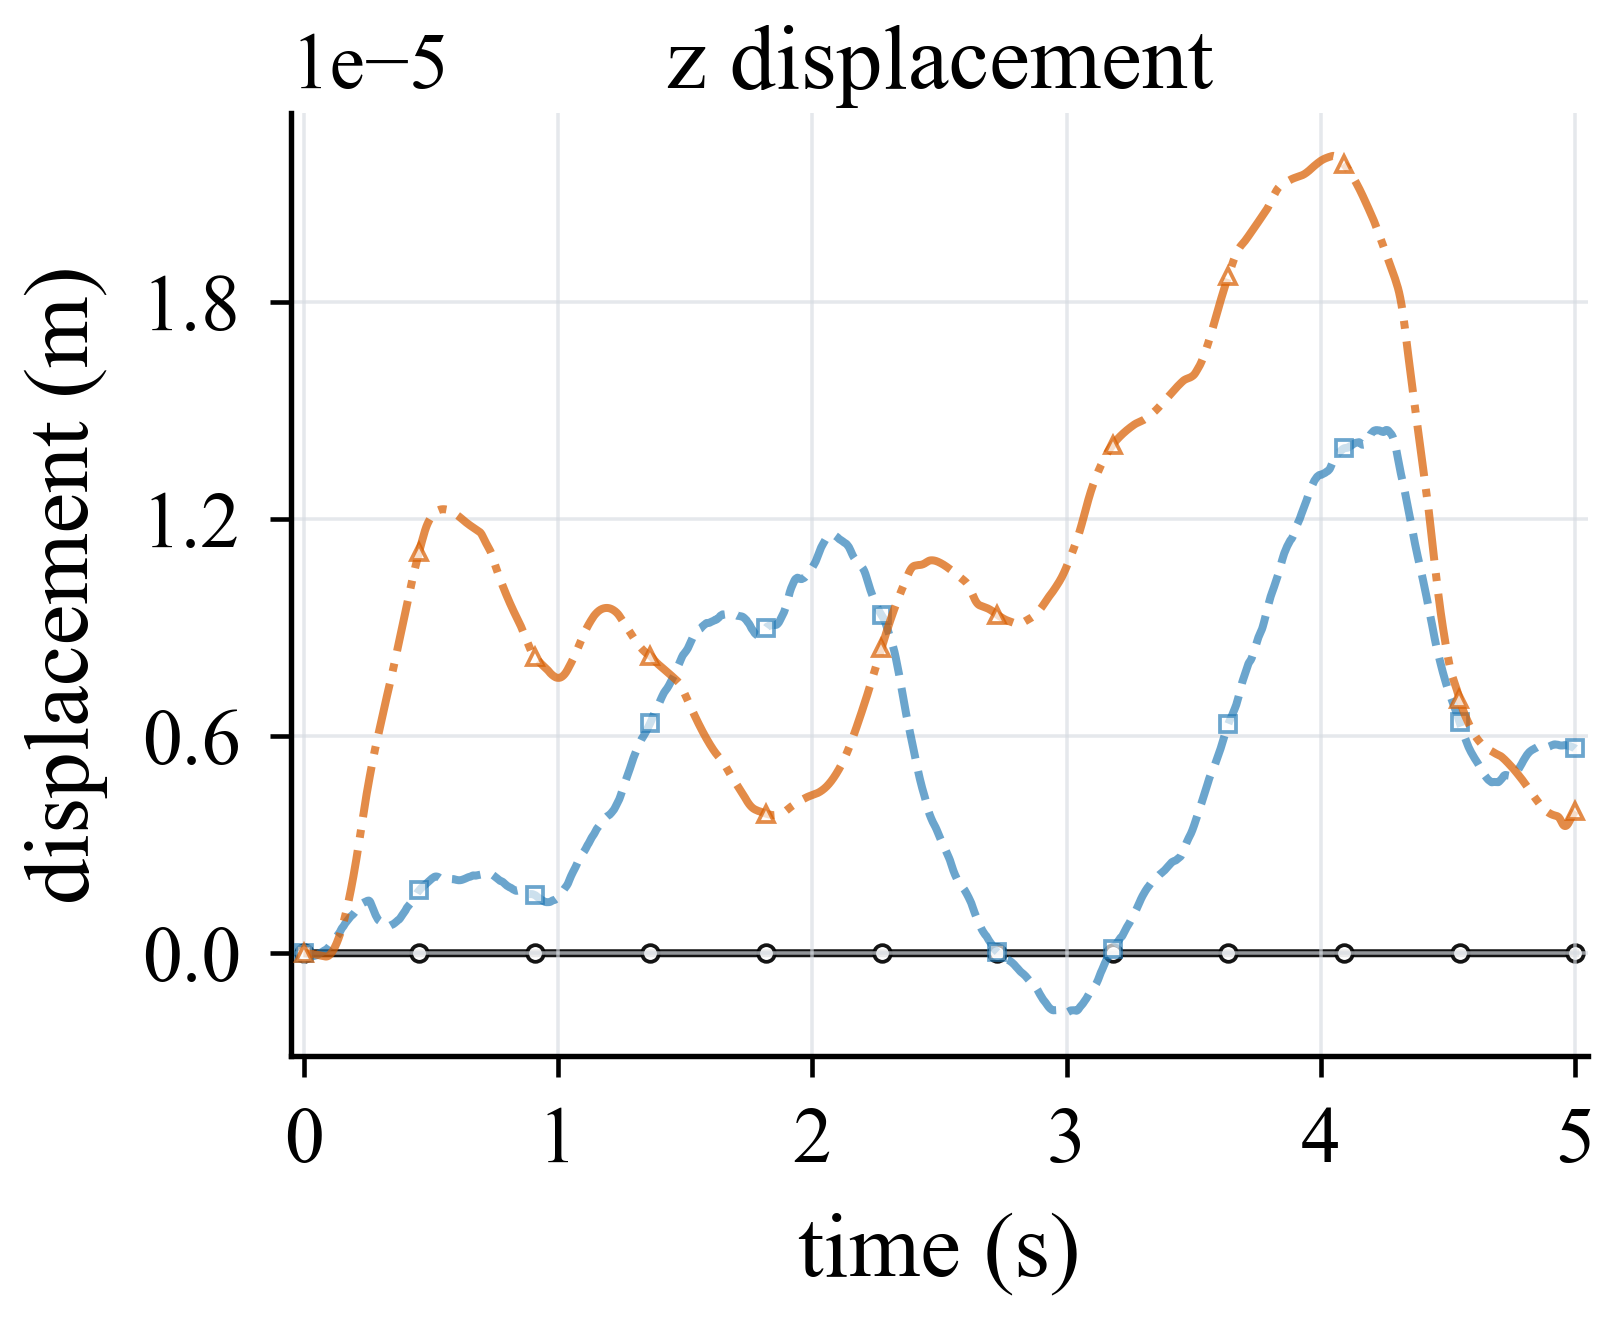
\includegraphics[width=\linewidth]{figures/calg_cmame_used/03_bearing_5s_z_displacement.png}
\end{minipage}
\caption{Bearing raceway validation over 5 s: ball displacement in the $x$, $y$, and $z$ directions. The \calg{} result is shown as the black solid curve; displacements are relative to each solver's initial ball coordinate.}
\label{fig:bearing_displacement}
\end{figure}

\begin{figure}[t]
\centering
\begin{minipage}{0.32\linewidth}
\centering

\includegraphics[width=\linewidth]{figures/calg_cmame_used/03_bearing_5s_x_velocity.png}
\end{minipage}\hfill
\begin{minipage}{0.32\linewidth}
\centering

\includegraphics[width=\linewidth]{figures/calg_cmame_used/03_bearing_5s_y_velocity.png}
\end{minipage}\hfill
\begin{minipage}{0.32\linewidth}
\centering
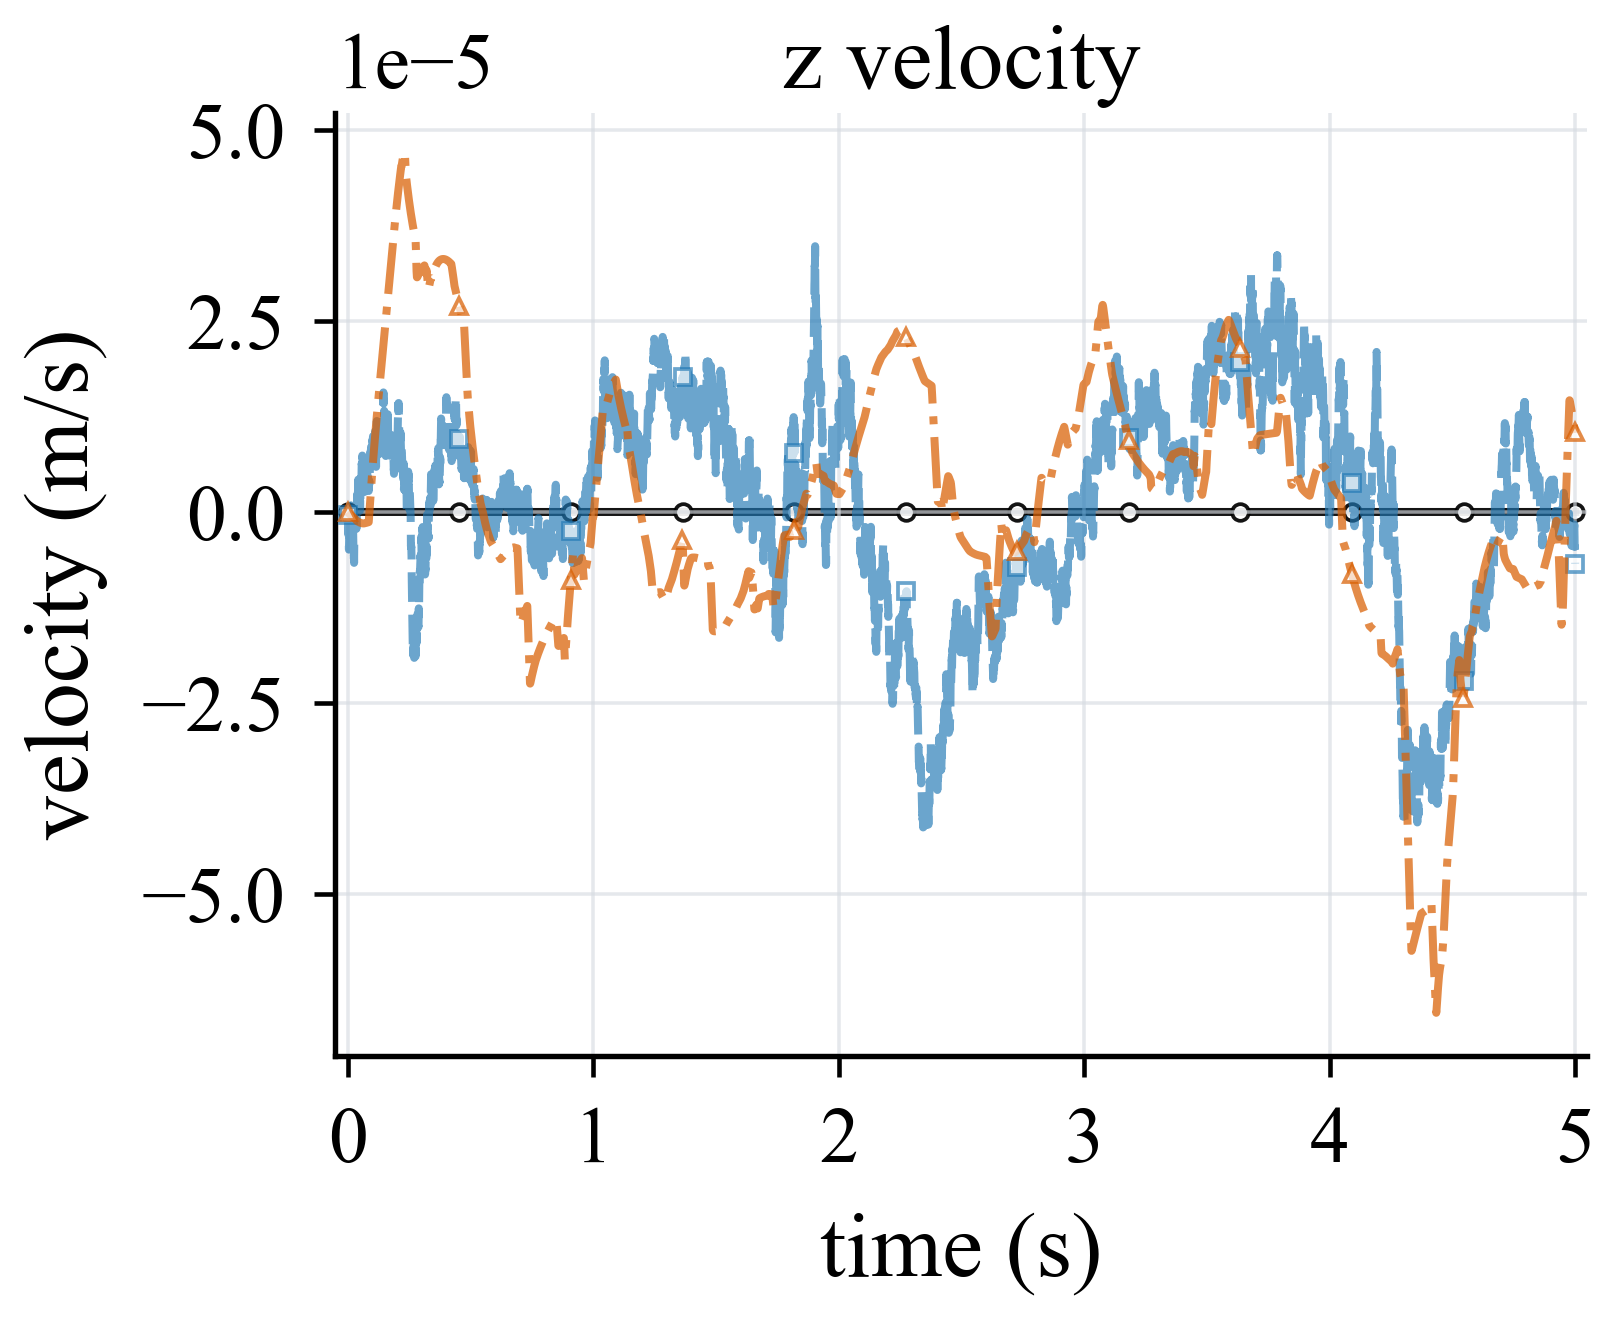
\includegraphics[width=\linewidth]{figures/calg_cmame_used/03_bearing_5s_z_velocity.png}
\end{minipage}
\caption{Bearing raceway validation over 5 s: ball velocity in the $x$, $y$, and $z$ directions. The \calg{} result is shown as the black solid curve.}
\label{fig:bearing_velocity}
\end{figure}

\begin{figure}[t]
\centering
\begin{minipage}{0.32\linewidth}
\centering
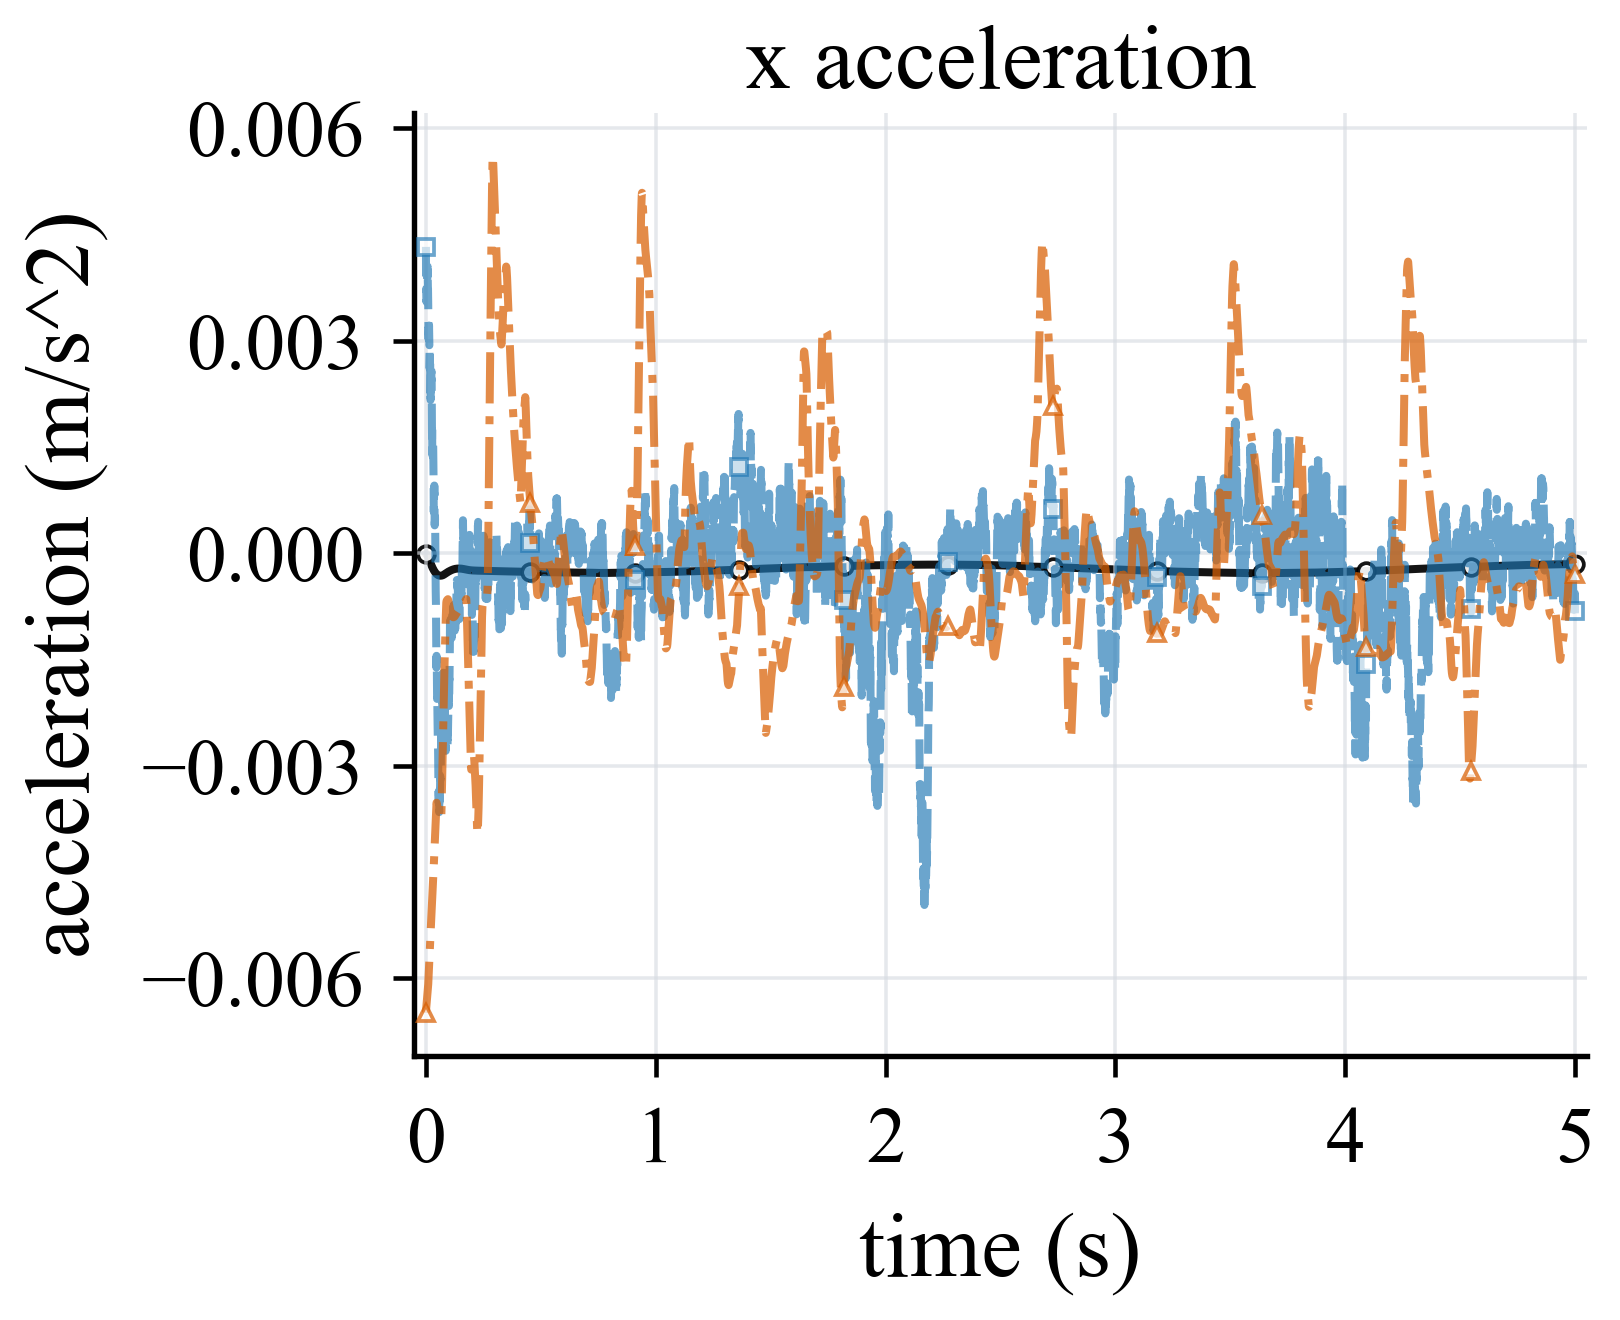
\includegraphics[width=\linewidth]{figures/calg_cmame_used/03_bearing_5s_x_acceleration.png}
\end{minipage}\hfill
\begin{minipage}{0.32\linewidth}
\centering

\includegraphics[width=\linewidth]{figures/calg_cmame_used/03_bearing_5s_y_acceleration.png}
\end{minipage}\hfill
\begin{minipage}{0.32\linewidth}
\centering
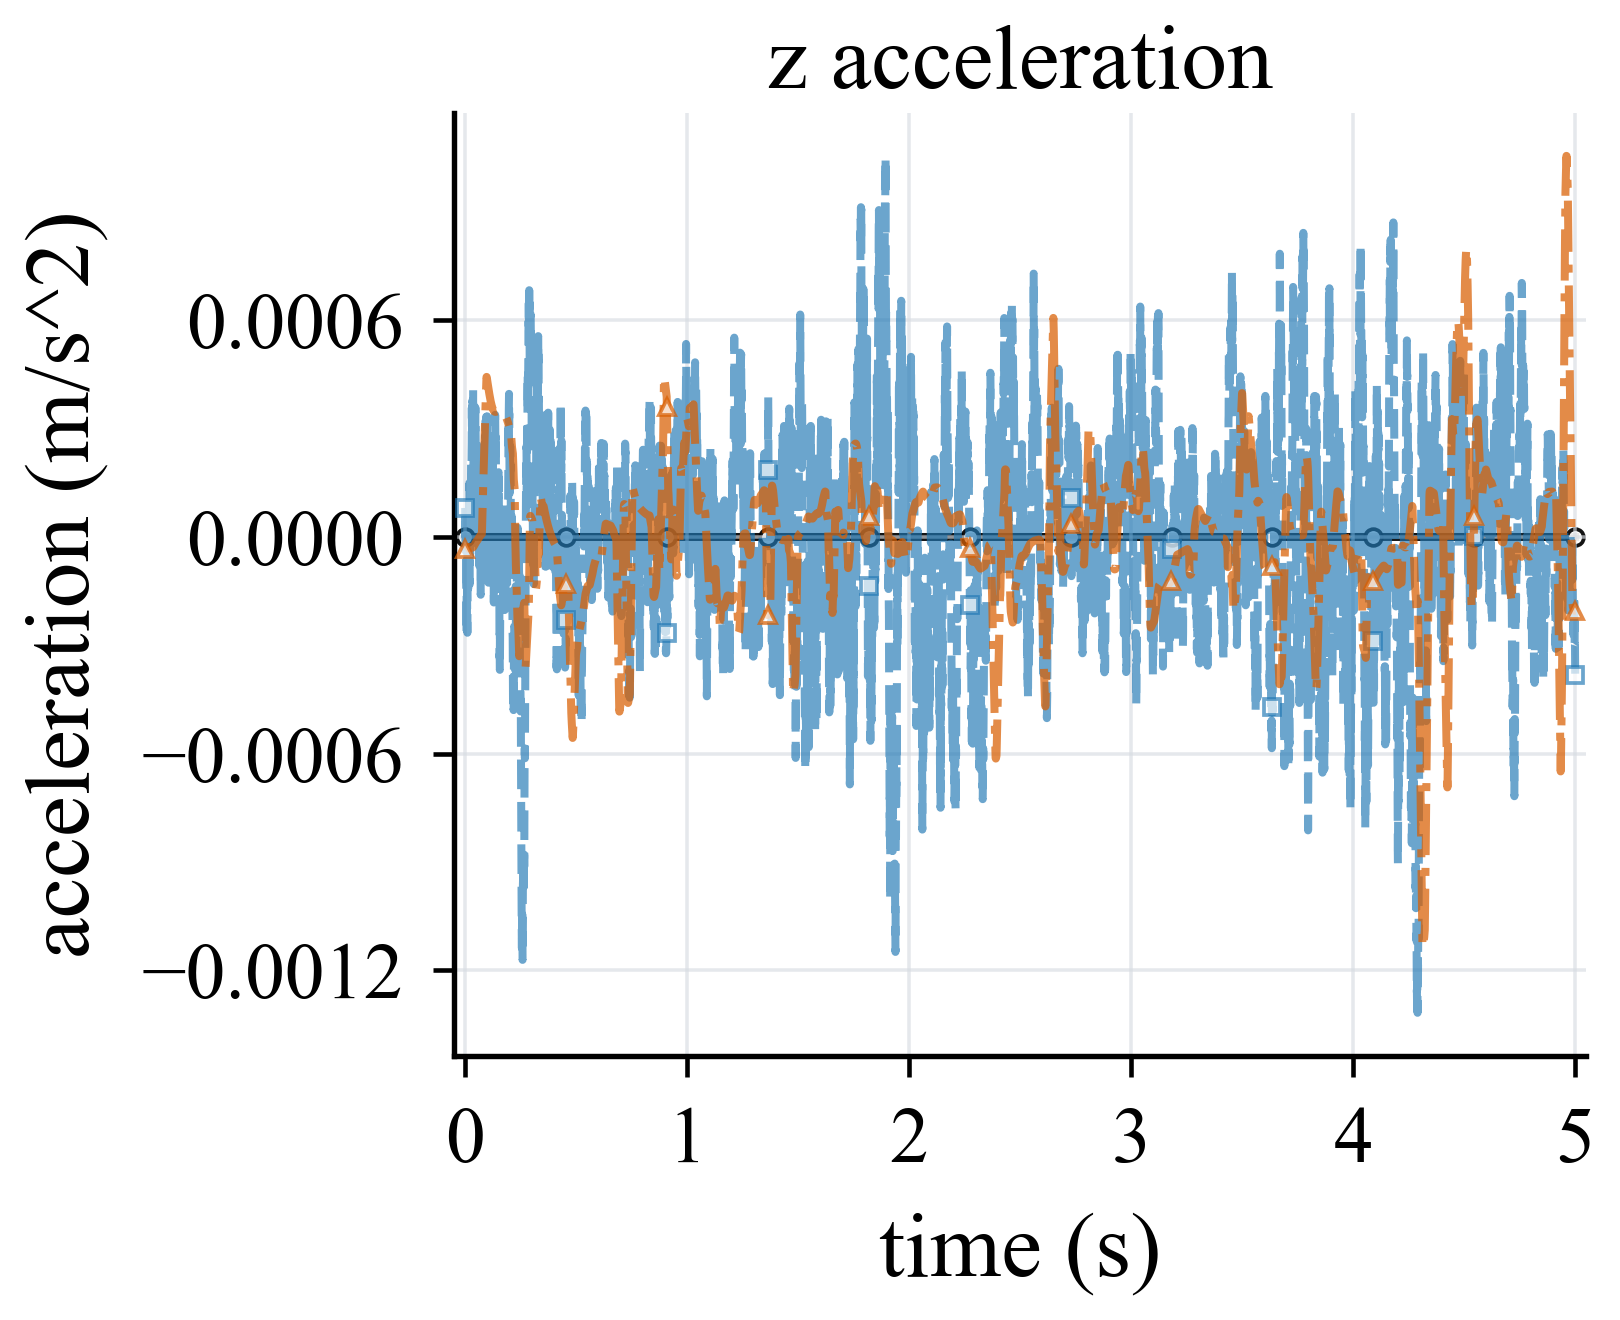
\includegraphics[width=\linewidth]{figures/calg_cmame_used/03_bearing_5s_z_acceleration.png}
\end{minipage}
\caption{Bearing raceway validation over 5 s: ball acceleration in the $x$, $y$, and $z$ directions. For \calg{} and Recurdyn, acceleration is taken from the exported solver channels; for Chrono it is evaluated from the reported contact force. The plotted curves use a 41-frame centered average for visualization.}
\label{fig:bearing_acceleration}
\end{figure}
\FloatBarrier

Together, the three external validation scenes show that the same \calg{}--SDF contact samples can drive consistent rigid-motion trends in selected engineering settings while preserving the smoother contact-normal and friction-response behavior established in the direct contact-geometry comparison.

\begin{table}[t]
\centering
\caption{Contact-geometry replay diagnostic on the three external validation trajectories. The locked \calg{} detector trajectory is replayed and the contact-geometry module is changed while keeping the rigid state and friction parameters fixed.}
\label{tab:chrono_backend_diagnostic}
{\setlength{\tabcolsep}{4pt}
\begin{tabular}{l l r r r}
\toprule
Model & Metric & \begin{tabular}[c]{@{}c@{}}Linear-triangle\\BVH\end{tabular} & \begin{tabular}[c]{@{}c@{}}PN-triangle\\BVH\end{tabular} & \calg{} \\
\midrule
Guide slot & $\Delta n_{\max}$ (deg) & 17.98 & 1.04 & 0.945 \\
& $\Delta F_{n,\max}$ (N) & 302.09 & 245.44 & 261.20 \\
& $\Delta F_{t,\max}$ (N) & 11.98 & 11.33 & 10.96 \\
& $v_t$ jitter (m/s) & $2.25\times10^{-2}$ & $2.69\times10^{-3}$ & $2.74\times10^{-3}$ \\
\midrule
Ball-and-socket pendulum & $\Delta n_{\max}$ (deg) & 4.67 & 0.0618 & 0.0176 \\
& $\Delta F_{n,\max}$ (N) & 0.562 & 0.0467 & 0.0467 \\
& $\Delta F_{t,\max}$ (N) & 0.0229 & 0.00415 & 0.00415 \\
& $v_t$ jitter (m/s) & $1.34\times10^{-4}$ & $1.34\times10^{-4}$ & $1.33\times10^{-4}$ \\
\midrule
Bearing raceway & $\Delta n_{\max}$ (deg) & 0 & 0 & $1.63\times10^{-3}$ \\
& $\Delta F_{n,\max}$ (N) & 0.506 & 0.504 & 0.505 \\
& $\Delta F_{t,\max}$ (N) & $1.26\times10^{-4}$ & $5.38\times10^{-5}$ & $5.38\times10^{-5}$ \\
& $v_t$ jitter (m/s) & $6.33\times10^{-5}$ & $6.15\times10^{-5}$ & $6.16\times10^{-5}$ \\
\bottomrule
\end{tabular}
}
\end{table}

Table~\ref{tab:chrono_backend_diagnostic} connects the external validation scenes back to the paper's contact-geometry mechanism by replaying the selected rigid states with the three geometry modules. This contact-geometry replay diagnostic is not an external-solver error table; it changes only the contact-geometry module along the same trajectory. The Guide slot and Ball-and-socket pendulum diagnostics reproduce the expected Linear-triangle BVH failure mode: the facet-based module causes much larger normal and normal-force jumps under the same friction parameters. The Bearing raceway diagnostic is intentionally retained as a neutral control: the locked trajectory of the Bearing raceway scene spans only a small angular interval, so it is not a discriminating normal-jump test, but it verifies that the three contact-geometry evaluations remain comparable in a smooth near-steady raceway segment.

\subsection{CALG C++ simulation efficiency}

The Python engineering suite is useful for development but not an appropriate efficiency baseline. To measure simulation efficiency more fairly, all three selected validation scenes were run through the same native CALG C++ implementation and compared with Chrono wall-clock time and Recurdyn solver-reported CPU Time. Table~\ref{tab:cpp_efficiency} reports CALG simulation time without full CSV trace export and excludes one-time geometry preprocessing such as dense SDF construction. In all three scenes, the reported CALG timing uses local mesh/CALG detector traversal followed by configuration-space SDF refinement and normalized surface-contact response quadrature for the signed gap, normal, and frictional response, rather than a faster analytic-provider-only replay.

\begin{table}[t]
\centering
\caption{Simulation efficiency comparison for Chrono, Recurdyn, and CALG. Chrono values are wall-clock times for the corresponding simulations; Recurdyn values are solver-reported CPU Time; CALG values are native C++ simulation times and exclude one-time geometry preprocessing such as dense SDF construction. The Time/CALG rows report each simulation time divided by the CALG time for the same case. Host hardware: AMD Ryzen 9 5900X, 12 cores/24 threads, Windows 11 Pro 64-bit.}
\label{tab:cpp_efficiency}
\begin{tabular}{l l r r r}
\toprule
Case & Metric & Chrono & Recurdyn & CALG \\
\midrule
Guide slot & Time (s) & 0.87 & 12.40 & 0.66 \\
& Time/CALG & $1.31\times$ & $18.75\times$ & $1.00\times$ \\
\midrule
Ball-and-socket pendulum & Time (s) & 150.22 & 454.83 & 20.98 \\
& Time/CALG & $7.16\times$ & $21.68\times$ & $1.00\times$ \\
\midrule
Bearing raceway & Time (s) & 49.43 & 61.19 & 18.66 \\
& Time/CALG & $2.65\times$ & $3.28\times$ & $1.00\times$ \\
\bottomrule
\end{tabular}
\end{table}

Figure~\ref{fig:cpp_efficiency} visualizes the same simulation efficiency data. These values should be read as implemented validation benchmark timings, not as a general engine-level comparison: Chrono, Recurdyn, and CALG use different contact discretizations and regularizations. Within this benchmark, CALG achieves higher simulation efficiency than Chrono in all three selected scenes.

\begin{figure}[t]
\centering
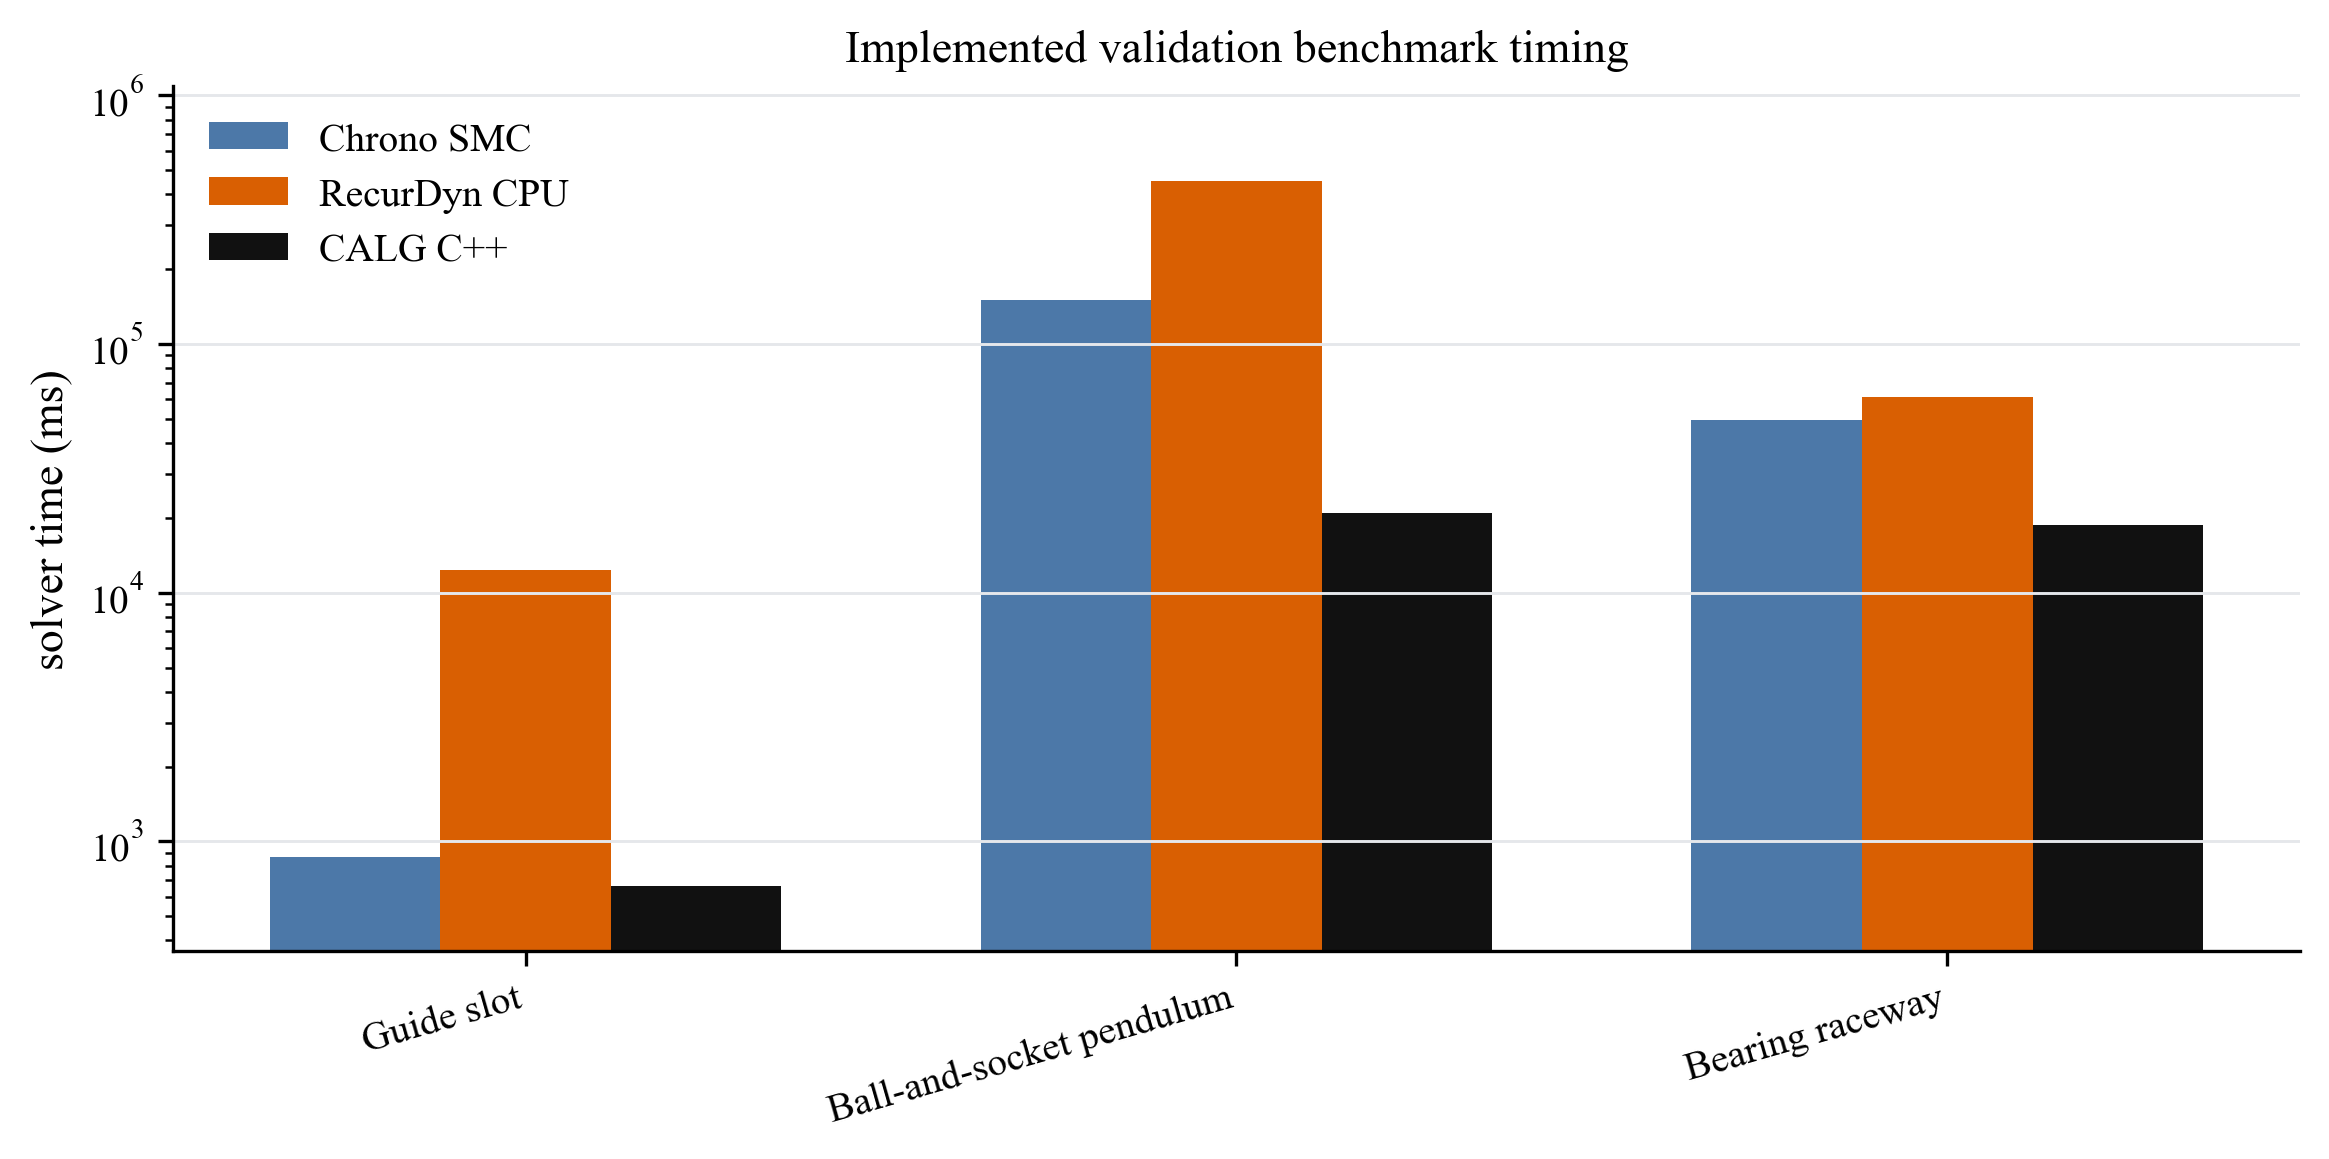
\includegraphics[width=0.78\linewidth]{figures/calg_cmame_used/04_efficiency_wall_time.png}
\caption{Simulation efficiency per selected validation scene. CALG uses no-CSV simulation timing and excludes one-time geometry preprocessing such as dense SDF construction; Recurdyn uses solver-reported CPU Time. All three CALG rows include local mesh/CALG detector traversal, configuration-space SDF signed refinement, and normalized surface-contact response quadrature. Timing ratios are reported in Table~\ref{tab:cpp_efficiency} and describe this implemented validation benchmark only, not an engine-wide comparison.}
\label{fig:cpp_efficiency}
\end{figure}

\FloatBarrier

\subsection{Scope of the current evidence}

The current evidence supports a specific claim: for smooth engineering contact, the \calg{}--SDF pipeline provides smoother signed gaps, normals, and tangential frames for rigid frictional response than fixed faceted or fixed-tessellation contact-geometry modules. The executable results in this paper use rigid-body contact samples, detector-driven candidate selection, configuration-space SDF refinement in the C++ validation implementation, and regularized Coulomb friction. This distinction is important for interpreting the method as a contact-geometry formulation rather than as an engine-wide replacement for established multibody dynamics engines.

\section{Conclusion}
\label{sec:conclusion}

This paper addresses frictional contact artifacts caused by discontinuous or tessellation-dependent contact geometry. The key idea is to couple a contact-aligned local graph detector with a configuration-space signed-distance response layer. The local graph supplies the signed gap, contact normal, and tangent frame from the local contact geometry, while the SDF layer provides the smooth signed gap and gradient normal used by the rigid friction law.

The reported results support the method at three levels. Analytic inclined-plane controls verify that the rigid-friction update reproduces static sticking, kinetic sliding, and the expected threshold transition. Dynamic rigid-friction tests then show that Linear-triangle BVH and PN-triangle BVH produce substantially larger normal jumps, normal-force jumps, friction-force jumps, and tangential-speed jitter than \calg{} in the four engineering scenes. Chrono and Recurdyn comparisons confirm trajectory-level agreement in displacement and velocity trends in three selected engineering scenes. In the C++ simulation efficiency benchmark, the \calg{}--SDF implementation achieves higher simulation efficiency than Chrono in all three selected scenes, with the comparison limited by different contact regularizations.

The present limitation is scope rather than the central geometric mechanism. The implementation and validation focus on rigid frictional contact over smooth analytic or CAD-like patches, with a configuration-space SDF used as the signed-distance response layer in the final C++ implementation. Sparse or adaptive SDF storage and production-grade multiphysics integration remain future work.

\section*{CRediT authorship contribution statement}
\textbf{Lijing Wang}: Conceptualization, Methodology, Software, Investigation, Writing - original draft.
\textbf{Ping Zhou}: Methodology, Validation, Formal analysis, Writing - review and editing.
\textbf{Wei Fan}: Validation, Resources, Writing - review and editing.
\textbf{Hui Ren}: Conceptualization, Supervision, Project administration, Funding acquisition.

\section*{Declaration of competing interest}
The authors declare that they have no known competing financial interests or personal relationships that could have appeared to influence the work reported in this paper.

\section*{Data availability}
The code, input definitions, scripts, generated figures, and numerical result artifacts required to reproduce the reported tables are available in the public repository at \url{https://github.com/W-Moorer/bff-rigid-contact.git}. The result files used in this draft are stored in the repository result directories v0.6, v0.9, v0.10, v0.11, v0.12, v0.13, v0.14, and v0.15. The repository includes source-result mappings, repository metadata, and a file-level manifest with SHA256 checksums.

\section*{Declaration of generative AI and AI-assisted technologies in the manuscript preparation process}
During the preparation of this work, the authors used OpenAI Codex to assist with manuscript restructuring, wording, consistency checks, and preparation of reproducibility and plotting scripts. No generative image model was used to create the scientific figures. After using this tool, the authors reviewed and edited the content as needed and take full responsibility for the content of the publication.

\section*{Acknowledgments}
This work was supported by the Open Funding of Automotive Industrial Software Openlab (Anhui).

\begin{thebibliography}{99}

\bibitem{johnson1985}
K. L. Johnson, \emph{Contact Mechanics}, Cambridge University Press, Cambridge, 1985. \doi{10.1017/CBO9781139171731}.

\bibitem{kikuchi1988}
N. Kikuchi and J. T. Oden, \emph{Contact Problems in Elasticity: A Study of Variational Inequalities and Finite Element Methods}, SIAM, Philadelphia, 1988. \doi{10.1137/1.9781611970845}.

\bibitem{laursen2002}
T. A. Laursen, \emph{Computational Contact and Impact Mechanics: Fundamentals of Modeling Interfacial Phenomena in Nonlinear Finite Element Analysis}, Springer, Berlin, 2003. \doi{10.1007/978-3-662-04864-1}.

\bibitem{wriggers2006}
P. Wriggers, \emph{Computational Contact Mechanics}, 2nd ed., Springer, Berlin, 2006. \doi{10.1007/978-3-540-32609-0}.

\bibitem{sauer2012}
R. A. Sauer and L. De Lorenzis, A computational contact formulation based on surface potentials, \emph{Computer Methods in Applied Mechanics and Engineering} 253 (2013) 369-395. \doi{10.1016/j.cma.2012.09.002}.

\bibitem{lu2011}
J. Lu, Isogeometric contact analysis: geometric basis and formulation for frictionless contact, \emph{Computer Methods in Applied Mechanics and Engineering} 200(5-8) (2011) 726-741. \doi{10.1016/j.cma.2010.10.001}.

\bibitem{temizer2011}
I. Temizer, P. Wriggers, and T. J. R. Hughes, Contact treatment in isogeometric analysis with NURBS, \emph{Computer Methods in Applied Mechanics and Engineering} 200(9-12) (2011) 1100-1112. \doi{10.1016/j.cma.2010.11.020}.

\bibitem{delorenzis2011}
L. De Lorenzis, I. Temizer, P. Wriggers, and G. Zavarise, A large deformation frictional contact formulation using NURBS-based isogeometric analysis, \emph{International Journal for Numerical Methods in Engineering} 87(13) (2011) 1278-1300. \doi{10.1002/nme.3159}.

\bibitem{li2020ipc}
M. Li, Z. Ferguson, T. Schneider, T. Langlois, D. Zorin, D. Panozzo, C. Jiang, and D. M. Kaufman, Incremental Potential Contact: Intersection- and inversion-free, large-deformation dynamics, \emph{ACM Transactions on Graphics} 39(4) (2020), Article 49. \doi{10.1145/3386569.3392425}.

\bibitem{li2021codimipc}
M. Li, D. M. Kaufman, and C. Jiang, Codimensional incremental potential contact, \emph{ACM Transactions on Graphics} 40(4) (2021) 1-24. \doi{10.1145/3450626.3459767}.

\bibitem{lan2021medialipc}
L. Lan, Y. Yang, D. M. Kaufman, J. Yao, M. Li, and C. Jiang, Medial IPC: accelerated incremental potential contact with medial elastics, \emph{ACM Transactions on Graphics} 40(4) (2021) 1-16. \doi{10.1145/3450626.3459753}.

\bibitem{ferguson2021rigidipc}
Z. Ferguson, M. Li, T. Schneider, F. Gil-Ureta, T. Langlois, C. Jiang, D. Zorin, D. M. Kaufman, and D. Panozzo, Intersection-free Rigid Body Dynamics, \emph{ACM Transactions on Graphics} 40(4) (2021), Article 183. \doi{10.1145/3450626.3459802}.

\bibitem{fang2024aipc}
Y. Fang, M. Li, Y. Cao, X. Li, J. Wolper, Y. Yang, and C. Jiang, Augmented Incremental Potential Contact for sticky interactions, \emph{IEEE Transactions on Visualization and Computer Graphics} 30(8) (2024) 5596-5608. \doi{10.1109/TVCG.2023.3295656}.

\bibitem{huang2024gipc}
K. Huang, F. M. Chitalu, H. Lin, and T. Komura, GIPC: Fast and stable Gauss-Newton optimization of IPC barrier energy, \emph{ACM Transactions on Graphics} 43(2) (2024), Article 23, 18 pages. \doi{10.1145/3643028}.

\bibitem{stiffgipc2025}
K. Huang, X. Lu, H. Lin, T. Komura, and M. Li, StiffGIPC: Advancing GPU IPC for Stiff Affine-Deformable Simulation, \emph{ACM Transactions on Graphics} 44(3) (2025) 1-20. \doi{10.1145/3735126}.

\bibitem{huang2025gcp}
Z. Huang, M. Paik, Z. Ferguson, D. Panozzo, and D. Zorin, Geometric Contact Potential, \emph{ACM Transactions on Graphics} 44(4) (2025) 1-24. \doi{10.1145/3731142}.

\bibitem{du2024smooth}
Y. Du, Y. Li, S. Coros, and B. Thomaszewski, Robust and artefact-free deformable contact with smooth surface representations, \emph{Computer Graphics Forum} 43(8) (2024) e15187. \doi{10.1111/cgf.15187}.

\bibitem{ferguson2023highorder}
Z. Ferguson, P. Jain, D. Zorin, T. Schneider, and D. Panozzo, High-Order Incremental Potential Contact for elastodynamic simulation on curved meshes, \emph{ACM SIGGRAPH Conference Proceedings} (2023) 1-11. \doi{10.1145/3588432.3591488}.

\bibitem{crespel2024fibres}
O. Crespel, E. Hohnadel, T. M\'{e}tivet, and F. Bertails-Descoubes, Contact detection between curved fibres: high order makes a difference, \emph{ACM Transactions on Graphics} 43(4) (2024), Article 132, 23 pages. \doi{10.1145/3658191}.

\bibitem{chen2024tdib}
X. Chen, C. Yu, X. Ni, M. Chu, B. Wang, and B. Chen, A time-dependent inclusion-based method for continuous collision detection between parametric surfaces, \emph{ACM Transactions on Graphics} 43(6) (2024) 1-11. \doi{10.1145/3687960}.

\bibitem{liu2024generalsdf}
P. Liu, Y. Zhang, H. Wang, M. K. Yip, E. S. Liu, and X. Jin, Real-time collision detection between general SDFs, \emph{Computer Aided Geometric Design} 111 (2024), Article 102305. \doi{10.1016/j.cagd.2024.102305}.

\bibitem{chen2025ogc}
A. H. Chen, J. Hsu, Z. Liu, M. Macklin, Y. Yang, and C. Yuksel, Offset Geometric Contact, \emph{ACM Transactions on Graphics} 44(4) (2025) 1-21. \doi{10.1145/3731205}.

\bibitem{pelletier2025trisdf}
J. Pelletier-Gu\'{e}nette, A. Mercier-Aubin, and S. Andrews, Real-Time Triangle-SDF Continuous Collision Detection, \emph{Proceedings of the ACM on Computer Graphics and Interactive Techniques} 8(4) (2025) 1-22. \doi{10.1145/3747862}.

\bibitem{stewart1996}
D. E. Stewart and J. C. Trinkle, An implicit time-stepping scheme for rigid body dynamics with inelastic collisions and Coulomb friction, \emph{International Journal for Numerical Methods in Engineering} 39(15) (1996) 2673-2691. \doi{10.1002/(SICI)1097-0207(19960815)39:15<2673::AID-NME972>3.0.CO;2-I}.

\bibitem{anitescu1997}
M. Anitescu and F. A. Potra, Formulating dynamic multi-rigid-body contact problems with friction as solvable linear complementarity problems, \emph{Nonlinear Dynamics} 14(3) (1997) 231-247. \doi{10.1023/A:1008292328909}.

\bibitem{jean1999}
M. Jean, The non-smooth contact dynamics method, \emph{Computer Methods in Applied Mechanics and Engineering} 177(3-4) (1999) 235-257. \doi{10.1016/S0045-7825(98)00383-1}.

\bibitem{acary2008}
V. Acary and B. Brogliato, \emph{Numerical Methods for Nonsmooth Dynamical Systems: Applications in Mechanics and Electronics}, Springer, Berlin, 2008. \doi{10.1007/978-3-540-75392-6}.

\bibitem{gavrea2008}
B. I. Gavrea, M. Anitescu, and F. A. Potra, Convergence of a class of semi-implicit time-stepping schemes for nonsmooth rigid multibody dynamics, \emph{SIAM Journal on Optimization} 19(2) (2008) 969-1001. \doi{10.1137/060675745}.

\bibitem{anitescu2010}
M. Anitescu and A. Tasora, An iterative approach for cone complementarity problems for nonsmooth dynamics, \emph{Computational Optimization and Applications} 47(2) (2010) 207-235. \doi{10.1007/s10589-008-9223-4}.

\bibitem{tasora2011}
A. Tasora and M. Anitescu, A matrix-free cone complementarity approach for solving large-scale, nonsmooth, rigid body dynamics, \emph{Computer Methods in Applied Mechanics and Engineering} 200(5-8) (2011) 439-453. \doi{10.1016/j.cma.2010.06.030}.

\bibitem{chakraborty2014}
N. Chakraborty, S. Berard, S. Akella, and J. C. Trinkle, A geometrically implicit time-stepping method for multibody systems with intermittent contact, \emph{The International Journal of Robotics Research} 33(3) (2014) 426-445. \doi{10.1177/0278364913501210}.

\bibitem{halm2024setvalued}
M. Halm and M. Posa, Set-valued rigid-body dynamics for simultaneous, inelastic, frictional impacts, \emph{The International Journal of Robotics Research} 43(10) (2024) 1594-1628. \doi{10.1177/02783649241236860}.

\bibitem{solanillas2024unilateral}
D. M. Solanillas Franc\'{e}s and J. K\"{o}vecses, A new formulation for the dynamics of rigid bodies with unilateral interactions, \emph{Mechanism and Machine Theory} 203 (2024), Article 105809. \doi{10.1016/j.mechmachtheory.2024.105809}.

\bibitem{luo2024symplectic}
J. Luo, X. Xu, X. Liu, and Z. Wu, A nonsmooth modified symplectic integration scheme for frictional contact dynamics of rigid--flexible multibody systems, \emph{Computer Methods in Applied Mechanics and Engineering} 420 (2024), Article 116726. \doi{10.1016/j.cma.2023.116726}.

\bibitem{chen2024contactforce}
W. Chen, X. Wang, Y. Liu, Y. Han, and Y. He, Modeling and verification of an improved contact force in multibody systems, \emph{Advances in Mechanical Engineering} 16(12) (2024), Article 16878132241307004. \doi{10.1177/16878132241307004}.

\bibitem{machado2012}
M. Machado, P. Moreira, P. Flores, and H. M. Lankarani, Compliant contact force models in multibody dynamics: Evolution of the Hertz contact theory, \emph{Mechanism and Machine Theory} 53 (2012) 99-121. \doi{10.1016/j.mechmachtheory.2012.02.010}.

\bibitem{flores2021}
P. Flores, Contact mechanics for dynamical systems: a comprehensive review, \emph{Multibody System Dynamics} 54(2) (2022) 127-177. \doi{10.1007/s11044-021-09803-y}.

\bibitem{corral2021}
E. Corral, R. Gismeros Moreno, M. J. G\'{o}mez Garc\'{i}a, and C. Castej\'{o}n, Nonlinear phenomena of contact in multibody systems dynamics: a review, \emph{Nonlinear Dynamics} 104(2) (2021) 1269-1295. \doi{10.1007/s11071-021-06344-z}.

\bibitem{tasora2016}
A. Tasora, R. Serban, H. Mazhar, A. Pazouki, D. Melanz, J. Fleischmann, M. Taylor, H. Sugiyama, and D. Negrut, Chrono: An open source multi-physics dynamics engine, in: \emph{High Performance Computing in Science and Engineering}, Lecture Notes in Computer Science, Springer, Cham, 2016, pp. 19-49. \doi{10.1007/978-3-319-40361-8_2}.

\bibitem{gilbert1988}
E. G. Gilbert, D. W. Johnson, and S. S. Keerthi, A fast procedure for computing the distance between complex objects in three-dimensional space, \emph{IEEE Journal on Robotics and Automation} 4(2) (1988) 193-203. \doi{10.1109/56.2083}.

\bibitem{gottschalk1996}
S. Gottschalk, M. C. Lin, and D. Manocha, OBBTree: A hierarchical structure for rapid interference detection, in: \emph{Proceedings of the 23rd Annual Conference on Computer Graphics and Interactive Techniques}, 1996, pp. 171-180. \doi{10.1145/237170.237244}.

\bibitem{mirtich1998}
B. Mirtich, V-Clip: fast and robust polyhedral collision detection, \emph{ACM Transactions on Graphics} 17(3) (1998) 177-208. \doi{10.1145/285857.285860}.

\bibitem{teschner2005}
M. Teschner, S. Kimmerle, B. Heidelberger, G. Zachmann, L. Raghupathi, A. Fuhrmann, M.-P. Cani, F. Faure, N. Magnenat-Thalmann, W. Strasser, and P. Volino, Collision detection for deformable objects, \emph{Computer Graphics Forum} 24(1) (2005) 61-81. \doi{10.1111/j.1467-8659.2005.00829.x}.

\bibitem{bridson2002}
R. Bridson, R. Fedkiw, and J. Anderson, Robust treatment of collisions, contact and friction for cloth animation, \emph{ACM Transactions on Graphics} 21(3) (2002) 594-603. \doi{10.1145/566654.566623}.

\bibitem{harmon2008}
D. Harmon, E. Vouga, R. Tamstorf, and E. Grinspun, Robust treatment of simultaneous collisions, in: \emph{ACM SIGGRAPH 2008 Papers}, 2008, Article 23, pp. 1-4. \doi{10.1145/1399504.1360622}.

\bibitem{redon2002}
S. Redon, A. Kheddar, and S. Coquillart, Fast continuous collision detection between rigid bodies, \emph{Computer Graphics Forum} 21(3) (2002) 279-288. \doi{10.1111/1467-8659.00587}.

\bibitem{brochu2012}
T. Brochu, E. Edwards, and R. Bridson, Efficient geometrically exact continuous collision detection, \emph{ACM Transactions on Graphics} 31(4) (2012) 1-7. \doi{10.1145/2185520.2185592}.

\bibitem{pabst2010}
S. Pabst, A. Koch, and W. Stra{\ss}er, Fast and scalable CPU/GPU collision detection for rigid and deformable surfaces, \emph{Computer Graphics Forum} 29(5) (2010) 1605-1612. \doi{10.1111/j.1467-8659.2010.01769.x}.

\bibitem{wang2021ccd}
B. Wang, Z. Ferguson, T. Schneider, X. Jiang, M. Attene, and D. Panozzo, A large-scale benchmark and an inclusion-based algorithm for continuous collision detection, \emph{ACM Transactions on Graphics} 40(5) (2021) 1-16. \doi{10.1145/3460775}.

\bibitem{delorenzis2014}
L. De Lorenzis, P. Wriggers, and T. J. R. Hughes, Isogeometric contact: a review, \emph{GAMM-Mitteilungen} 37(1) (2014) 85-123. \doi{10.1002/gamm.201410005}.

\bibitem{osher1988}
S. Osher and J. A. Sethian, Fronts propagating with curvature-dependent speed: algorithms based on Hamilton-Jacobi formulations, \emph{Journal of Computational Physics} 79(1) (1988) 12-49. \doi{10.1016/0021-9991(88)90002-2}.

\bibitem{curless1996}
B. Curless and M. Levoy, A volumetric method for building complex models from range images, in: \emph{Proceedings of the 23rd Annual Conference on Computer Graphics and Interactive Techniques}, 1996, pp. 303-312. \doi{10.1145/237170.237269}.

\bibitem{jones2006}
M. W. Jones, J. A. B{\ae}rentzen, and M. Sramek, 3D distance fields: a survey of techniques and applications, \emph{IEEE Transactions on Visualization and Computer Graphics} 12(4) (2006) 581-599. \doi{10.1109/TVCG.2006.56}.

\bibitem{vlachos2001pn}
A. Vlachos, J. Peters, C. Boyd, and J. L. Mitchell, Curved PN triangles, \emph{Proceedings of the 2001 Symposium on Interactive 3D Graphics} (2001) 159-166. \doi{10.1145/364338.364387}.

\end{thebibliography}

\end{document}
